% Working research article, revised September 28, 2026.
% Suggested compilation: latexmk -pdf -interaction=nonstopmode -halt-on-error Garamon_research_article_2026-09-27_en.tex
\documentclass[11pt,a4paper]{article}
\usepackage[T1]{fontenc}
\usepackage[utf8]{inputenc}
\usepackage[english]{babel}
\usepackage{lmodern}
\usepackage{amsmath,amssymb}
\usepackage{booktabs,tabularx}
\usepackage{graphicx}
\usepackage{pgfplots}
\usepackage{placeins}
\usepackage{needspace}
\pgfplotsset{compat=1.18}
\usepackage[margin=22mm]{geometry}
\usepackage[colorlinks=true,urlcolor=blue,linkcolor=blue,citecolor=blue]{hyperref}
\Urlmuskip=0mu plus 1mu\relax
\emergencystretch=1.5em
\newcommand{\Cl}{\mathrm{Cl}}
\newcommand{\supp}{\operatorname{supp}}
\newcommand{\code}[1]{\texttt{#1}}

\title{Adaptive Exact Computation in Garamon.jl:\\
Audit of the C++ Generator and Initial Evaluations}
\author{}
\date{September 28, 2026}

\begin{document}

\maketitle
\begin{abstract}
The appropriate geometric algebra product depends on operand supports, requested outputs, and reuse horizon as well as ambient dimension. We audit the Garamon C++ generator and examine a pure Julia implementation with exact traversals, support joins, structured representations, and reusable workspaces. Each technique is presented with its intended workload, preparation cost, correctness evidence, and measured result. Here ``exact'' means that no mathematical contribution is deliberately omitted; floating-point rounding still applies.

A PerfChecker sweep qualifies 3\,256 cases in dimensions 2--256. A separate workspace campaign qualifies 687 cases, including 150 warmed kernels with no recorded allocation. Prepared ternary joins lose on the first call in ten tested dimensions yet win all twenty measured cells at 1\,024 calls. Replacing \code{BigInt} masks with \code{UInt128} lowers a paired 65D targeted-kernel median from 2.129 to 0.179~\(\mu\)s. A native EGA3 catalog sharply reduces the first prepared-product latency for known topologies after restart; new topologies still compile. These cases show why preparation and requested output must enter the comparison.

The binary-ranking prototype wins 35/36 short-episode configurations against a prepared plan, but none at 1\,024 products. A single-pass B1W workspace variant reduces sparse-output allocation bytes by about 30--35\%; a separate long-horizon replay favors it in 48/48 paired comparisons, with median earlier/new ratio 1.106. Other exact structural prototypes are validated on their stated fixtures, but no general strategy threshold follows.

Two order-reversed Julia 1.13/Clang 18 packed-kernel replays each qualify 64/64 cases and 1\,984 warm samples. At 10\,000 products, Julia wins 4/8 paired comparisons (median Julia/C++ ratio 1.032); the upstream C++ \code{Mvec} product has a different, unmatched contract. A paired packed CPU/GPU screen qualifies 384 cases: the GPU wins 34/48 complete episodes at 8\,192 products, with median CPU/GPU ratio 1.027. CUPTI traces find host-output copies longer than kernels in two fixtures. Registering a fresh pinned host output wins only 30/72 long-horizon comparisons against ordinary GPU output in the broader twelve-dimension screen. A further matched screen with four CPU threads reverses the long-horizon ranking: at 8\,192 products the GPU beats the sequential CPU in 57/72 complete episodes but the four-thread CPU in only 13/72. Under a \emph{different} exact contract, four packed operand sets stay resident while $R$ products accumulate into one final host output. Fusing those $R$ products into one GPU kernel wins 72/72, 63/72, and 71/72 complete episodes against the $R$-kernel GPU at $(H,R)=(32,32),(1\,024,8),(1\,024,32)$, but only 22/72 against CPU4 at $(32,32)$. A 12D reversal in the broad screen changes sign in six focused replays, with unknown cause. A separate CUDA Graph pilot reuses an $R$-kernel sequence for $Q$ identical-value sums: it often beats ordinary submissions but loses all 16 paired comparisons to fusion at each of three workloads. A fixed-support screen across 129--8\,192D qualifies 320 cases. A separate exact rerun after grouped algebra validation cuts 8\,192D fused preparation from 34.43 to 2.28~ms and the complete episode from 45.84 to 12.50~ms; within that rerun, fusion beats CPU4 in all 40 paired comparisons at each of two workloads. No automatic GPU routing or general language winner follows.
\par\smallskip\noindent\textbf{Keywords:} geometric algebra, Clifford product, sparse computation, support join, workspace, Julia compilation.
\end{abstract}

\section{Introduction}
An algebra $\Cl(V,G)$ of dimension $n$ has $2^n$ possible coordinates, yet an individual computation may touch only a few blades. At a fixed dimension, the occupied supports and requested outputs determine how much work is useful. A scalar coefficient may justify a direct join where a complete multivector justifies another traversal. Ambient dimension alone is therefore insufficient for strategy selection. Other relevant variables are the form and conditioning of $G$, the grade distribution, support size and locality, the number of outputs, and the reuse horizon. Preparation time, JIT compilation, allocations, retained memory, RAM, task count, and potentially VRAM belong to the cost model.

Garamon.jl currently preserves every contribution to an exact output. Here ``exact'' means that the algorithm deliberately omits no contribution; floating-point rounding still applies. An approximate strategy with speculative pruning would need a separate API and an explicit error contract, rather than a silent substitution for the exact mode.

This article asks which paths the C++ generator and Julia port provide, when supports and requested outputs make full expansion unnecessary, and when plans and buffers repay their preparation cost. We audit the code and report algorithms and measurements that separate preparation, compilation, and execution whenever the protocol allows. Undermeasured areas remain research questions, without an automatic routing threshold. Section~\ref{sec:techniques} links each technique to its motivating workload, expected cost, evidence, and comparison needed for adoption.

\section{Related work}
The Garamon generator combines precomputed work with recursive traversal of a virtual prefix tree~\cite{breuils2019,garamoncpp}. The arithmetic bounds of Breuils, Nozick, and Sugimoto address products of two full homogeneous multivectors~\cite{breuils2020}. We also study sparse supports, targeted outputs, and repeated sequences, which impose different contracts.

Outside geometric algebra, FFTW planning illustrates program selection~\cite{fftw}. Database joins~\cite{leapfrog}, sparse tensor planning~\cite{galley}, and sparse workspaces~\cite{sparseworkspace} motivate avoiding unnecessary intermediate products. Equality saturation~\cite{egg} and SHAP analysis of selectors~\cite{shap} are potential tools only when their costs and transformation proofs are included. Performance from those domains cannot be transferred to Garamon by analogy alone.

\section{Method: exact products and path selection}
For an orthogonal basis $e_1,\ldots,e_n$ with $e_i^2=g_i$, let $e_A$ denote the ordered blade with mask $A$. Then
\begin{equation}
e_Ae_B=\sigma(A,B)\left(\prod_{i\in A\cap B}g_i\right)e_{A\triangle B},
\qquad \sigma(A,B)\in\{-1,1\},
\label{eq:blade}
\end{equation}
where $\triangle$ denotes symmetric difference. A zero metric factor, an impossible output grade, or an output that was not requested can eliminate a path by proof. For coefficient $K$ of $(ab)c$, candidate masks satisfy $A\triangle B\triangle C=K$. Traversing the two smaller supports determines the third mask by XOR; factors and signs are still evaluated in the original product order. The \code{join3} join samples no eligible triple. It draws on relational join traversal~\cite{leapfrog}, but does not implement Leapfrog Triejoin or inherit its bounds.

Two implementations have different preparation costs. The expression route \code{join3} recomputes one targeted output. \code{TripleJoinPlan} prepares paths for several outputs once. A \code{TripleJoinWorkspace} reuses coefficient tables under explicit probe, path, and memory budgets. Its result is borrowed and overwritten by the next call.

The \code{test/triplejoin.jl} suite passes 223 assertions in dimensions 2, 3, 4, 6, 8, 12, 64, 65, 66, 127, 128, and 129, including degenerate metrics, support validation, and rejection of nonorthogonal bases. A separate 192-case PerfChecker comparison measures the plan; earlier I15.1 \code{join3} figures do not measure it.

Equation~\eqref{eq:blade} does not directly cover a nonorthogonal basis, where $e_i e_j=G_{ij}+e_i\wedge e_j$ for $i\ne j$. Such a basis requires an appropriate direct product or a basis change whose cost and numerical error are counted. Conservative grade propagation can rule out impossible intermediate supports before enumeration, but has its own preparation cost. Bounds for full homogeneous products~\cite{breuils2020} cannot be assigned without proof to a few scattered blades.

\section{Documented comparison of Garamon C++ and Garamon.jl}
We audit public commit \code{6267161} of the Garamon C++ repository~\cite{garamoncpp} against the generator paper~\cite{breuils2019}. The generator reads a configuration and metric, prepares mask-to-(grade,position) indexing, diagonalizes when needed, builds sparse change-of-basis matrices by grade, and emits a C++ library. A multivector stores its present grades in a list, with a dense coefficient vector per grade. Products use unrolled functions or recursive traversal of a \emph{virtual} prefix tree depending on grade and generation threshold. The audited paths neither materialize a tree of coefficient nodes nor memoize subproduct values~\cite{cppmain,cppindex,cppdispatch,cppmvec,cppgeometric,cppmetric}.

The current private GitLab \code{Garamon.jl} worktree is a pure Julia reimplementation, not a C++ wrapper. It supports bounded dense multivectors, dictionaries of active coefficients, direct products, \code{ProductPlan}, an expression DSL, targeted outputs, and bounded Julia code generation. Masks use \code{UInt64} through 64 directions, \code{UInt128} from 65 to 128, and \code{BigInt} beyond. Sparse orthogonal traversal does not require a global $2^n$ table. Explicit dense storage is limited to $n\leq20$, which does not imply that every admitted product is fast or within its execution budget.

Audited Julia files include \path{src/algebra.jl} for metrics, \path{src/multivectors.jl} for storage and masks, \path{src/plans.jl} for plans, \path{src/products.jl} and \path{src/dsl.jl} for targeted coefficients and expressions, and \path{src/generated.jl}, \path{src/workspace.jl}, and \path{src/triplejoin.jl} for generation and reusable buffers. They belong to the current worktree and do not all match initial commit \code{adf1dc5}.

\begin{table}[ht]
\centering\small
\begin{tabularx}{\linewidth}{@{}p{31mm}X X@{}}
\toprule
Aspect & Audited Garamon C++ & Observed Garamon.jl \\
\midrule
Preparation & Generate and compile a library for a configured algebra. & Specify the algebra at run time and prepare paths on demand; optional Julia specialization unrolls at most 256 paths. \\
Coefficients & Store present grades, with a dense vector within each grade. & Use bounded global dense storage or active masks only; prepared homogeneous blocks are possible. \\
Large dimension & Use $2^n$ indexing tables and \code{unsigned int} masks in the audited revision. & Use variable-width masks and explicit budgets; feasibility depends on the support. \\
Nonorthogonal\newline basis & Diagonalize, then apply outer transformation matrices by grade. & Use a direct general product and on-demand outer transformation under a budget. \\
Reuse & Generate code per algebra; no subproduct cache is observed in the audited paths. & Keep the plan, plan cache, generated program, and workspace separate. \\
\bottomrule
\end{tabularx}
\caption{Design comparison grounded in audited source files; this table does not compare language speed.}
\label{tab:cppjulia}
\end{table}

Semantic differences matter: a singular inverse raises an error in the Julia port, while the audited C++ path returns zero near its threshold. Julia public-kernel results and the C++/Julia benchmark have distinct contracts. The tests presented do not cover every C++ scenario; the accompanying technical comparison details evidence and capacity limits.

A first matched comparison ports the path loop of a packed Julia batch into an \emph{experimental} C++ kernel. Paths, accumulation order, tables, coefficients, outputs, and precision are held fixed, and warm measurements use the same Julia frontend. Two later replays retain paired raw samples in forward and reversed route orders. The actual generator-produced C++ \code{Mvec<double>} is timed \emph{descriptively} with its grade storage; it is not the paired language baseline for the packed route. Broader C++/Julia comparisons require first validating and optimizing each Julia technique, then implementing the same strategy in C++ and matching preparation, compilation, and measurement. Generated libraries were removed after each dimension~\cite{cppreport,cppreprise,cppmatchedreplay}.

\subsection{C++ and Julia: first matched packed kernel}
\label{sec:cppperf}
\paragraph{Why this experiment?}
Comparing languages with different algorithms confounds language cost with strategy cost. This pilot therefore ports the same packed path kernel and checks identical inputs, outputs, and operations before comparing times. An executable PerfChecker campaign validates 64/64 cases, with 31 warm samples per case, in EGA3 and EGA7. It covers two support families (\emph{mixed} and \emph{vectors}) and four independent batch sizes ($H=1,32,1024,10000$). An independent integer oracle checks every coefficient and support completeness; the workload is not a recurrence. The three \emph{matched} variants use the same path loop, accumulation order, \code{Float64} matrices, and output allocation through the Julia frontend: the public \code{run\_packed\_batch} function under Julia JIT, the same function after in-process \code{Base.precompile}, and an \emph{experimental} C++ port of that kernel. The packed C++ variant uses Clang 18.1.3 with \code{-O2}, \code{-march=native}, and floating-point contraction disabled~\cite{cppreport}. This comparison isolates one strategy; it does not represent the upstream C++ grade dispatcher.

\begin{figure}[ht]
\centering
\IfFileExists{exploratory_cpppacked.pdf}{\includegraphics[width=.92\linewidth]{exploratory_cpppacked.pdf}}{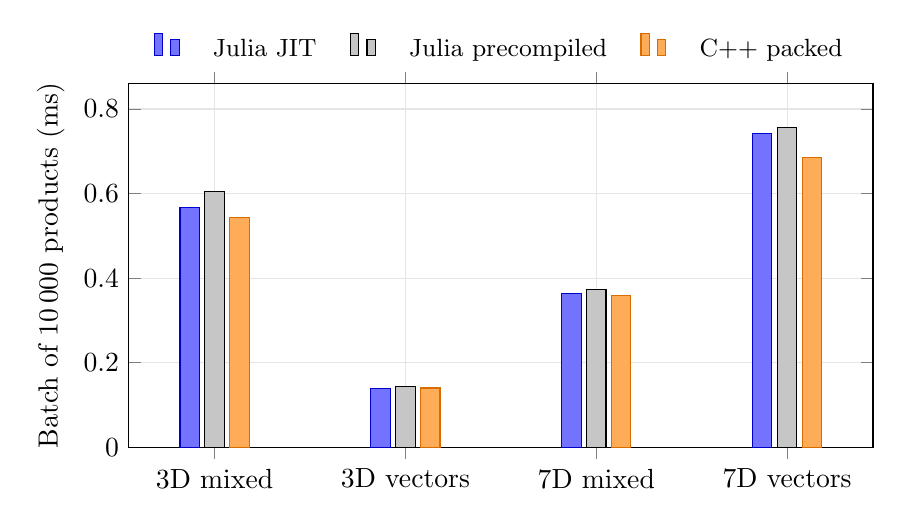
\begin{tikzpicture}
\begin{axis}[
  width=.91\linewidth,height=6.2cm,
  ybar,bar width=7pt,enlarge x limits=.15,
  ymin=0,ymax=.86,ytick={0,.2,.4,.6,.8},
  xtick={1,2,3,4},
  xticklabels={3D mixed,3D vectors,7D mixed,7D vectors},
  ylabel={Batch of 10\,000 products (ms)},
  grid=major,grid style={gray!20},
  legend style={at={(.5,1.03)},anchor=south,legend columns=3,column sep=10pt,draw=none,fill=white,font=\small},
]
\addplot+[fill=blue!55,draw=blue!80!black] coordinates
  {(1,.566444) (2,.138876) (3,.362696) (4,.741087)};
\addplot+[fill=gray!45,draw=black] coordinates
  {(1,.604970) (2,.142643) (3,.374018) (4,.756926)};
\addplot+[fill=orange!65,draw=orange!85!black] coordinates
  {(1,.543365) (2,.140069) (3,.358855) (4,.685747)};
\legend{Julia JIT,Julia precompiled,C++ packed}
\end{axis}
\end{tikzpicture}}
\caption{Warm medians for four 10\,000-product batches under one packed-kernel contract and the same frontend. ``Precompiled'' means in-process \code{Base.precompile}. This first pass ran alongside Étendue3D without CPU affinity; the bar differences do not establish a general winner. Data: \code{cpp-matched-warm.csv}.}
\label{fig:cpppacked}
\end{figure}

The four warm results are close: for EGA3 \emph{vectors}, the Julia JIT and packed C++ medians are 0.138876 and 0.140069~ms. The \emph{actual} \code{Mvec<double>} product from a Garamon-generated library was also executed and checked on 16 workloads. At $H=10000$, its medians in figure order are 2.724, 0.751, 1.746, and 1.385~ms. Grade storage, dispatch, and allocations differ, so these numbers do not yield a C++/Julia language ratio. We also time the native C++ executable's packed components, but do not subtract those times from frontend measurements to invent an ``FFI cost''. The separate C++-versus-C++ move experiment in Section~\ref{sec:moveperf} tests copies of temporary Eigen vectors in the audited \code{Mvec} path; it does not alter the packed comparison in Figure~\ref{fig:cpppacked}.

The observed first Julia JIT call takes 31.68--34.30~ms, almost entirely compilation. An in-process \code{Base.precompile} call costs 36.03--51.61~ms before the corresponding first products, which then report zero JIT time. This proves neither a total cold-start gain nor persistence of compiled code between sessions. Building the C++ generator takes about 18.66~s; building the packed library takes about 0.20~s; building the upstream library takes 1.32~s in EGA3 or 3.45~s in EGA7. Produced artifacts measured 3\,628\,956 and 7\,065\,214 bytes and were removed before the next dimension. A 256~MiB limit was monitored per dimension. These preparation phases cannot be added to a warm median to infer a crossover.

The first pass was unstable. At 7D \emph{mixed}, $H=1024$, the \emph{same} warm Julia function measured 17.452~\(\mu\)s after ordinary JIT and 34.956~\(\mu\)s after targeted precompilation, versus 16.999~\(\mu\)s for packed C++. This nearly twofold discrepancy does not establish a causal precompilation effect. Summaries of 31 samples survive, but individual times do not. Figure~\ref{fig:cpppacked} therefore remains a historical concurrent-load screen.

\paragraph{Why replay the matched kernel in both orders?}
The first screen cannot distinguish language effects from order and shared-machine activity. Two \emph{new, separate} Julia 1.13/Clang 18.1.3 campaigns repeat the same packed plan, operands, ordered contributions, \code{Float64} coefficients, and independently owned outputs, first in the original route order and then reversed. The C++ packed kernel receives prepared matrices and paths through \code{ccall}; both routes validate the batch in the Julia frontend. Each archive qualifies 64/64 cases and 1\,984 warm samples, with 31 samples per route and case, over EGA3/EGA7, \emph{mixed}/\emph{vectors} support, and $H=1,32,1\,024,10\,000$. The operator recorded no other user Julia/Garamon computation, which does not reserve a CPU core or certify fixed hardware conditions. The generator-produced \code{Mvec} timings remain in a separate, unmatched group. Generated C++ libraries and build trees were removed after each dimension~\cite{cppmatchedreplay}.

\begin{figure}[ht]
\centering
\IfFileExists{exploratory_cppreplay.pdf}{\includegraphics[width=.92\linewidth]{exploratory_cppreplay.pdf}}{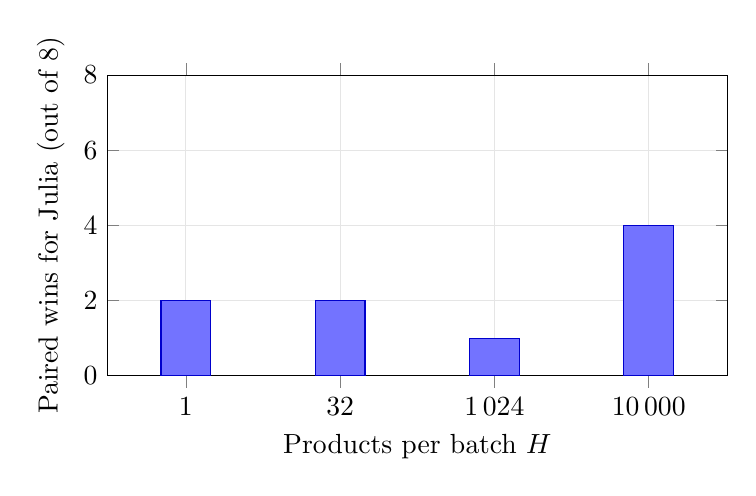
\begin{tikzpicture}
\begin{axis}[
 width=.78\linewidth,height=5.4cm,
 ybar,bar width=18pt,enlarge x limits=.17,
 ymin=0,ymax=8,ytick={0,2,4,6,8},
 xtick={1,2,3,4},xticklabels={1,32,1\,024,10\,000},
 xlabel={Products per batch \(H\)},
 ylabel={Paired wins for Julia (out of 8)},
 grid=major,grid style={gray!20},
]
\addplot+[fill=blue!55,draw=blue!80!black,mark=none] coordinates
 {(1,2) (2,2) (3,1) (4,4)};
\end{axis}
\end{tikzpicture}}
\caption{Julia JIT wins among four fixtures in each of two route orders, compared with the same experimental packed C++ kernel. Median within-pair Julia/C++ ratios are 1.054, 1.095, 1.064, and 1.032; below one favors Julia. Preparation and compilation are outside these warm medians. No bar represents upstream \code{Mvec}~\cite{cppmatchedreplay}.}
\label{fig:cppreplay}
\end{figure}

At $H=10\,000$, Julia wins 4/8 pairs across both orders; the median of the eight within-pair Julia/C++ ratios is 1.032 (range 0.974--1.136). EGA3 \emph{vectors} and EGA7 \emph{mixed} favor Julia in both orders, whereas EGA3 \emph{mixed} and EGA7 \emph{vectors} favor packed C++. Even without other declared user work, EGA7 \emph{mixed} at $H=1\,024$ changes substantially between orders; close ratios are not robust language effects. The archives retain cold times and build costs separately, which cannot be added to a warm median to create a lifecycle crossover. The precompiled Julia route is also kept separate: it wins only 1/8 pairs at $H=10\,000$ against C++ packed and has no general warm advantage in this grid. A broader, hardware-controlled matched campaign is still required before any language ranking~\cite{cppmatchedreplay}.
\FloatBarrier

\subsection{C++ versus C++: moving temporary Eigen buffers}
\label{sec:moveperf}
\paragraph{Why this experiment?}
The \code{Mvec} generated can copy an Eigen buffer when a temporary vector is inserted into its grade structure. The test isolates this copy cost into the same language and representation, then checks that the displacement retains all products. An isolated modification of the upstream \code{Mvec.hpp} replaces four insertions of a local \code{Kvec} by \code{std::move(kvec)} and includes \code{<utility>} ~\cite{cppmove}. Two sites concern access per index; two, the lazy creation of a grade vector. Each temporary is no longer used after insertion: the displacement transfers its Eigen buffer to the list node, instead of creating a second allocation and copying of the coefficients. The arithmetic order, support, grades and zero tests remain the same. The upstream clone remains intact; the modification is kept in an isolated C++ worktree, without publication or PR.

The native bench opposes \emph{the same C++} before and after this change. It takes back EGA3/EGA7, support supports \emph{mixed} / \emph{vectors} , $H=1,32,1024,10000$ and writes in a pre-allocated matrix all the structurally possible coefficients for these supports. The inputs and the entire oracle are identical in both variants; their preparation and allocation of the matrix are excluded from the kernel. Upstream and modified executables check in total 67\,840 exact products, including all basic blades pairs and 256 pairs of additional multivectors per dimension and executable; the tests inspect all the coefficients, including zeros. A separate test confirms the transfer of address of the buffer Eigen and the absence of aliases with the operands. The demonstrated domain is \code{Float64} , Euclidean metric, 3D and 7D~\cite{cppmove} .

\begin{figure}[ht]
\centering
\IfFileExists{exploratory_cppmovealloc.pdf}{\includegraphics[width=.92\linewidth]{exploratory_cppmovealloc.pdf}}{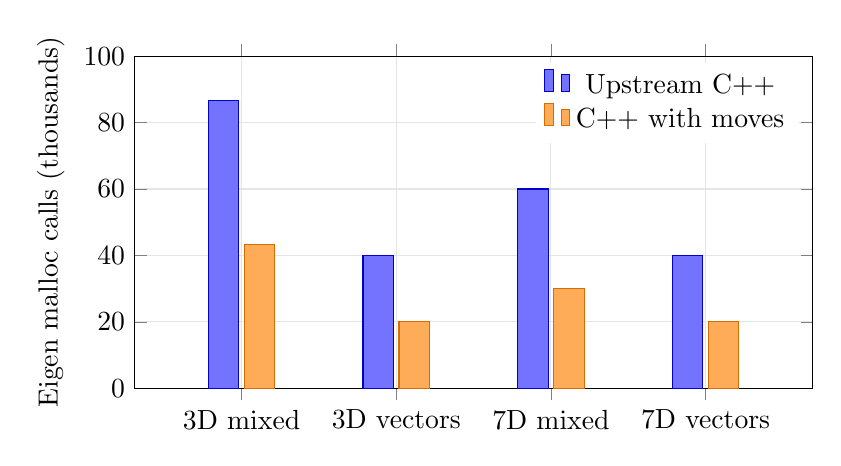
\begin{tikzpicture}
\begin{axis}[
  width=.84\linewidth,height=5.8cm,
  ybar,bar width=11pt,enlarge x limits=.23,
  ymin=0,ymax=100,ytick={0,20,40,60,80,100},
  xtick={1,2,3,4},
  xticklabels={3D mixed,3D vectors,7D mixed,7D vectors},
  ylabel={Eigen malloc calls (thousands)},
  grid=major,grid style={gray!20},
  legend style={at={(.98,.98)},anchor=north east,draw=none,fill=white},
]
\addplot+[fill=blue!55,draw=blue!80!black] coordinates
  {(1,86.666) (2,40) (3,60) (4,40)};
\addplot+[fill=orange!65,draw=orange!85!black] coordinates
  {(1,43.333) (2,20) (3,30) (4,20)};
\legend{Upstream C++,C++ with moves}
\end{axis}
\end{tikzpicture}}
\caption{Eigen-buffer \code{malloc} calls over 10\,000 products. Two orders and three repetitions give identical counts. Node \code{new} allocations are unchanged; combined \code{malloc} and \code{new} calls fall by one third in all 32 matched groups. These are instrumented allocation counts, not peak RSS. Data: \code{cpp-move-allocations.csv}.}
\label{fig:cppmovealloc}
\end{figure}

The 32 paired groups (16 loads in two orders), i.e. 192 meter observations, exactly divide the requested number and bytes of the Eigen buffers by two; the nodes allocations do not change. The \emph{Cumulative} \code{malloc+new} bytes in EGA3 \emph{mixed} to $H=10000$ go from 5\,839\,960 to 3\,786\,640; the other families and horizons follow the same mechanism. Meters exclude inputs, oracle, output and internal calls to unintercepted shared libraries. The time binary does not instrument allocations, so as not to slow down the kernel it times.

\begin{table}[ht]
\centering\small
\begin{tabular}{@{}lrr@{}}
\toprule
Workload, $H=10000$ & Baseline then move & Move then baseline \\
\midrule
EGA3 mixed & 2.525 $\to$ 2.217 & 2.441 $\to$ 1.981 \\
EGA3 vectors & 0.692 $\to$ 0.527 & 0.689 $\to$ 0.521 \\
EGA7 mixed & 1.310 $\to$ 1.013 & 1.307 $\to$ 1.019 \\
EGA7 vectors & 0.951 $\to$ 0.807 & 0.933 $\to$ 0.784 \\
\bottomrule
\end{tabular}
\caption{Medians of 101 observations per variant and order, in milliseconds per batch. Each arrow runs from upstream C++ to modified C++. Timings are exploratory under Étendue3D load and separate from the packed C++/Julia comparison. Data: \code{cpp-move-times.csv}.}
\label{tab:cppmovetimes}
\end{table}

The move variant was faster in both passes, but Étendue3D continued to share the machine despite pinning the controller to logical core P0. For EGA7 vectors at $H=32$, the modified/upstream ratios were 0.985 and 0.827 in the two orders. This campaign retained all 101 individual times per variant, unlike the first packed benchmark. Without full activity control and before/after calibration, reduced allocations are the firm result here; the size of any timing gain awaits an isolated rerun. Generated objects were removed after each dimension, within the monitored 256~MiB disk ceiling~\cite{cppmove}.
\FloatBarrier

\section{Plans, workspaces, JIT, and reuse horizons}
A structural plan stores masks, $(i,j,k)$ paths, and metric factors, but no operand values.

A \code{ProductWorkspace} preallocates input and output coefficient arrays and a sparse result multivector. Each call checks the algebra and supports, refreshes coefficients, clears outputs, and accumulates every eligible path. The returned result is \emph{borrowed}: the next call overwrites it, so retaining a history requires copying. A mutable workspace belongs to one task. Admission checks the estimated object size against \code{max\_bytes} and one quarter of observed free system memory. This one-time check is neither a process RSS ceiling nor a bound on JIT code or arbitrary-precision coefficient growth. Sparse-workspace research~\cite{sparseworkspace} motivates the design without proving that one format is optimal for Garamon.

Four lifetimes differ: the algebra and any change of basis; the structural plan; mutable buffers; and compiled machine code. A generated product encodes path indices in a Julia type parameter, while factors and coefficients remain values. Constructing that object does not compile its first execution. Package precompilation or an application image may cover known specializations, but a new support structure or type can still trigger JIT~\cite{juliaprecompile}. We therefore distinguish an algebra known before startup from structures discovered during a session. The I15.6 protocol below tests both. Saving a \code{ProductPlan} alone does not establish persistence of native code across processes.

For $H$ calls in one process under the same output contract, the cost comparison is
\begin{equation}
C_{\mathrm{plan}}+C_{\mathrm{workspace}}+C_{\mathrm{JIT,prep}}
  +H\,t_{\mathrm{prep}}
\quad\text{versus}\quad C_{\mathrm{JIT,direct}}+H\,t_{\mathrm{direct}},
\label{eq:amort}
\end{equation}
If compilation has already been paid in a warm scenario, its terms vanish from that scenario. A fresh process must measure them separately. This is a decision model, not a threshold inferred from the campaigns below. A portfolio approach, as in FFTW planning~\cite{fftw}, helps only when selection and preparation pay for themselves on the actual workload.

\section{Implemented techniques: motivation, experiment, and result}
\label{sec:techniques}
Each technique begins with the workload that motivates it, followed by the experiment, measurements, and validity limits. Figures compare routes that compute the same requested output within one campaign; times from separate campaigns are not pooled. Here, \emph{implemented} means present in the studied Julia source, \emph{measured} means evaluated on a named corpus and output contract, and \emph{hypothesis} means that a speed gain has not been demonstrated. References motivate mechanisms; performance numbers come from Garamon measurements. A gain for one targeted coefficient does not imply a gain for a full multivector, and warm execution time does not include preparation, compilation, or output copying unless stated.

\subsection{Density, sparse supports, and grade blocks}
\paragraph{Why this technique?}
The C++ generator of Breuils, Nozick, and Fuchs~\cite{breuils2019} stores present grades with a dense array of size $\binom nk$ for each grade. Garamon.jl also offers globally dense storage bounded by $n\leq20$, a dictionary of active masks, plans for homogeneous grade blocks, and a sorted list for some outer products. Sparse tensor compilers such as TACO~\cite{taco} and Finch~\cite{finch} motivate separating format, traversal, and computation, but do not solve Clifford signs, cancellation, or grade changes. Dense storage targets small $n$ or well-populated grades; dictionaries target scattered supports; prepared grade blocks target repeated calls with homogeneous structure.
\paragraph{Tests, results, and limitations.}
Dense storage pays for zeros and potentially $2^n$ slots. Sparse storage pays for lookup, hashing, and less regular locality. A prepared block pays enumeration and memory before its first value. In a homogeneous 12D grade-3-by-grade-3 family, a plan covers 48\,400 paths, occupies 1.81~MiB, and costs 9.23~ms to prepare, followed by 0.24~ms per integer product. Eight changing supports cost 11.02~ms including preparation, versus 27.14~ms with direct computation and 19.36~ms with a rebuilt plan per support~\cite{roadmap}. For a top-grade wedge coefficient in 12D, the sorted \code{UInt64} list takes 0.93 versus 5.42~\(\mu\)s over 56 masks; a \code{BigInt} prototype in 66D loses to the join~\cite{roadmap}. These cases do not define a universal density threshold. A further protocol must match operation, output, support, and type, include conversion and block construction, and measure peak memory and reuse horizon; full middle grades and changing supports are needed.

\subsection{C++ prefix recursion and grade planning}
\paragraph{Why this technique?}
In the audited C++ code, products for some small grades are unrolled; others traverse a virtual prefix tree whose nodes do not store persistent coefficients~\cite{cppgeometric,cppdispatch}. This avoids emitting every combination as source code. The bounds of Breuils, Nozick, and Sugimoto~\cite{breuils2020} concern two \emph{full} homogeneous multivectors. Recursion is therefore a relevant baseline for complete products or many active grades. Grade propagation may eliminate impossible outputs before traversing support paths.
\paragraph{Tests, results and limitations.}
Recursion, grade indices, and dense tables have costs even for sparse operands. In the Julia I15.1 campaign at scattered 256D supports, four requested outputs take 140.7~\(\mu\)s by recursion versus 223.6~\(\mu\)s by \code{join3}. For a scalar output, the times reverse: 130.3 versus 87.6~\(\mu\)s (Table~\ref{tab:dimensions}). These are two \emph{Julia} paths, not a measurement of upstream C++ recursion. The first executable C++ benchmark measures upstream \code{Mvec} separately and pairs a packed port with Julia; it does not isolate identical recursive strategies. A future language comparison must match strategy, metric, supports, coefficients, precision, outputs, and timed scope, then report generation, compilation, first call, warm execution, and disk cost by dimension. Any grade-propagation preparation must be charged to its route.

\subsection{XOR join and \code{TripleJoinPlan}}
\paragraph{Why this technique?}
For a diagonal metric, the output mask of a binary product is $K=A\triangle B$: given $A$ and $K$, the mask $B$ is fixed. For $(ab)c$, $C=A\triangle B\triangle K$. Traversing two supports and probing the third can replace full intermediate expansion with an exact join. This resembles multiway relational joins~\cite{leapfrog}, without inheriting their complexity bounds. The target is one or a few requested outputs from sparse operands in a diagonal algebra. An implemented \code{TripleJoinPlan} stores structural $(i,j,k)$ paths for several outputs; its workspace refreshes values and keeps mutable buffers private to each task.
\paragraph{Tests, results and limitations.}
A join pays for probes, signs, and metric factors; several outputs may repeat paths. For a scattered scalar at 256D, measured \code{join3} takes 87.6 versus 1\,643.7~\(\mu\)s for a complete product. For four requested outputs in the same family, it loses to recursion, 223.6 versus 140.7~\(\mu\)s. The \code{TripleJoinPlan} passes 223 correctness assertions. A paired 192-case benchmark compares that plan, \code{join3}, and two complete routes on the \emph{same} three operands and outputs. Including preparation, the plan loses at $H=1$ in all ten tested dimensions but wins twenty cells at $H=1\,024$ (Section~\ref{sec:tripleperf}). Supports activate only two to four directions, and some long-horizon cells have one timing sample. Confirmation needs both binary intermediate plans, recursion, richer supports, owned-output materialization, and an isolated rerun that records accepted paths, JIT, and memory. This join rejects nonorthogonal metrics, which require another product formula.

\subsection{Dimensions and requested outputs}
\paragraph{Why this experiment?}
The dimension alone does not say whether the useful calculation is dense or sparse. This scan requires when a targeted output avoids enough work to compensate for its address, and when the complete product remains preferable, with support and explained budgets. The continuous scan validated 3\,256 cases and recorded 6\,944 budget exclusions. It covers each integer from 2 to 256 with at most twelve bitrators dispersed plus the scalar, 2 to 70 in two other sparse families, 2 to 11 for the full grade 2 and 2 to 5 for the fully occupied entry. Four strategies and one or four outputs are compared. The limit 256 is an experimental envelope, not an intrinsic saturation of sparse products. The times of the table~\ref{tab:dimensions} are medians per batch, without preparation; the first compilation and allocations are separately shown in the associated dimension-sweep CSV files and archived qualification records.

\begin{table}[ht]
\centering\small
\begin{tabular}{@{}lrrrr@{}}
\toprule
Family, $n$, output & Full & Recursive & Grades & \code{join3} \\
\midrule
Scattered sparse, 2, scalar & 1.9 & 9.8 & 14.6 & 5.2 \\
Scattered sparse, 5, scalar & 29.3 & 33.3 & 40.9 & 17.6 \\
Scattered sparse, 64, scalar & 211.5 & 34.4 & 41.4 & 20.5 \\
Scattered sparse, 65, scalar & 1\,380.5 & 77.8 & 103.9 & 75.0 \\
Scattered sparse, 256, scalar & 1\,643.7 & 130.3 & 130.3 & 87.6 \\
Scattered sparse, 256, four outputs & 1\,674.3 & 140.7 & 144.8 & 223.6 \\
Full grade 2, 11, scalar & 4\,915.9 & 277.8 & 339.8 & 269.7 \\
Full grade 2, 11, four outputs & 4\,849.5 & 342.1 & 407.7 & 958.7 \\
\bottomrule
\end{tabular}
\caption{Microseconds per batch in campaign I15.1. At this source revision, dimension 65 switched from \code{UInt64} to \code{BigInt}; a later campaign measured \code{UInt128}.}
\label{tab:dimensions}
\end{table}

\begin{figure}[ht]
\centering
\IfFileExists{exploratory_sorties.pdf}{\includegraphics[width=.92\linewidth]{exploratory_sorties.pdf}}{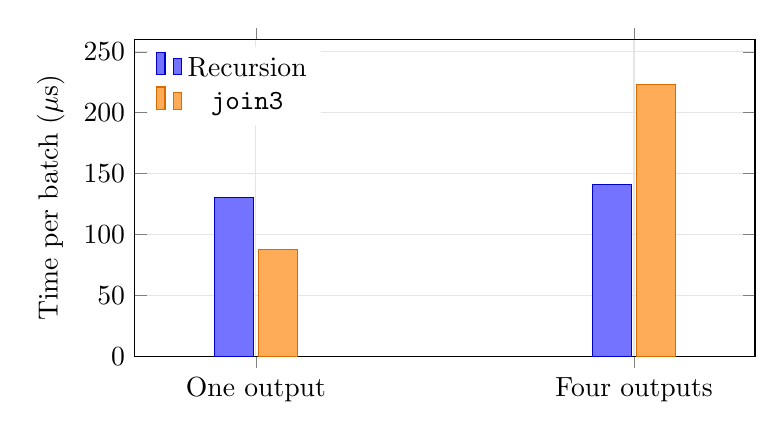
\begin{tikzpicture}
\begin{axis}[
  width=.78\linewidth,height=5.6cm,
  ybar,bar width=14pt,enlarge x limits=.32,
  ymin=0,ymax=260,ytick={0,50,100,150,200,250},
  xtick={1,4},xticklabels={One output,Four outputs},
  ylabel={Time per batch (\(\mu\)s)},
  grid=major,grid style={gray!20},
  legend style={at={(.02,.98)},anchor=north west,draw=none,fill=white},
]
\addplot+[fill=blue!55,draw=blue!80!black] coordinates {(1,130.3) (4,140.7)};
\addplot+[fill=orange!65,draw=orange!85!black] coordinates {(1,87.6) (4,223.6)};
\legend{Recursion,\code{join3}}
\end{axis}
\end{tikzpicture}}
\caption{In sparse 256D cases, the number of requested outputs reverses the ranking of two Julia paths. Two of the four outputs are structurally zero in this family. Exploratory I15.1 timings use the same \code{BigInt} mask revision in both cells.}
\label{fig:sorties}
\end{figure}

For one output, \code{join3} can save expansion; for four outputs with 256 dimensions, it loses in front of the recursion. The two odd outputs of the set of four are structurally null in exclusively paired families. The automatic thresholds therefore require confirmation on other grades, metrics and passing orders.
\FloatBarrier

\subsection{Prepared ternary join: first comparison}
\label{sec:tripleperf}
\paragraph{Why this experiment?}
A join of three factors avoids the materialization of some intermediate results, but its plan costs to prepare. The experiment looks for the horizon where this preparation amortizes for the same sets and outputs support. The TripleJoin campaign validates 192 cases in dimensions $2,3,4,5,8,12,32,65,128,129$ , for one or four outputs and horizons $H=1,32,1024$; 10\,000 calls are added in 65 and 128D. The three routes evaluated calculate the same coefficients of $(ab)c$: two complete products then extraction, \code{join3} called for each output, and \code{TripleJoinPlan} with Workspace. The three inputs change values at each step but keep their support sets. The independent \code{Int64} oracle checks the amounts of the trace; the entire small corpus remains exactly representative in \code{Float64} . The preparation of the artifact between \emph{once} in each measured trace and the output is accumulated in a table of the caller.

\begin{table}[ht]
\centering\small
\begin{tabular}{@{}rrcc@{}}
\toprule
Outputs & $H$ & Wins: direct / \code{join3} / plan & Median ratio: plan/\code{join3} \\
\midrule
1 & 1 & 2 / 8 / 0 & 14.039 \\
1 & 32 & 0 / 5 / 5 & 1.113 \\
1 & 1024 & 0 / 0 / 10 & 0.139 \\
4 & 1 & 5 / 5 / 0 & 5.427 \\
4 & 32 & 0 / 1 / 9 & 0.306 \\
4 & 1024 & 0 / 0 / 10 & 0.033 \\
\bottomrule
\end{tabular}
\caption{First paired TripleJoin comparison: per-cell medians include preparation. The ratio is the median of within-dimension ratios; values below one favor the prepared plan. Data: \code{perf-triplejoin/warm.csv}.}
\label{tab:tripleperf}
\end{table}

\begin{figure}[ht]
\centering
\IfFileExists{exploratory_tripleamort.pdf}{\includegraphics[width=.92\linewidth]{exploratory_tripleamort.pdf}}{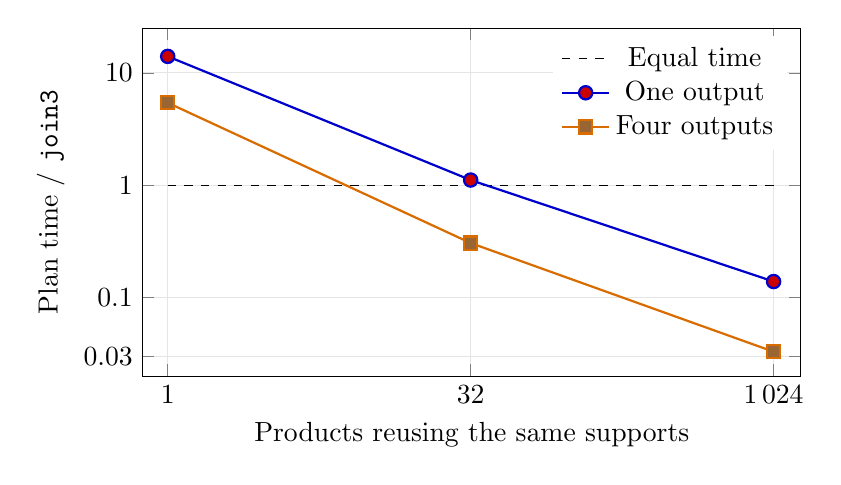
\begin{tikzpicture}
\begin{loglogaxis}[
  width=.82\linewidth,height=6.0cm,
  xmin=.75,xmax=1400,ymin=.02,ymax=25,
  xtick={1,32,1024},xticklabels={1,32,1\,024},
  ytick={.03,.1,1,10},yticklabels={0.03,0.1,1,10},
  xlabel={Products reusing the same supports},
  ylabel={Plan time / \code{join3}},
  grid=major,grid style={gray!20},
  legend style={at={(.98,.98)},anchor=north east,draw=none,fill=white},
]
\addplot+[black,dashed,mark=none] coordinates {(1,1) (1024,1)};
\addplot+[blue!80!black,thick,mark=*,mark size=2.4pt] coordinates
  {(1,14.039) (32,1.113) (1024,.139)};
\addplot+[orange!85!black,thick,mark=square*,mark size=2.4pt] coordinates
  {(1,5.427) (32,.306) (1024,.033)};
\legend{Equal time,One output,Four outputs}
\end{loglogaxis}
\end{tikzpicture}}
\caption{Amortization of the ternary plan on the TripleJoin corpus. The plotted median within-dimension ratio includes preparation; values below one favor the plan. Segments connect only the three measured horizons and do not establish an interpolated threshold. Timings are exploratory.}
\label{fig:tripleamort}
\end{figure}

The plan loses the first call in all tested dimensions. At 65D with one output and $H=32$, \code{join3} remains faster, taking 0.095 versus 0.329~ms per episode. At 8D with four outputs and $H=32$, the plan wins, 0.085 versus 0.353~ms. At $H=1\,024$, it wins all twenty cells of this corpus and allocates fewer \emph{cumulative} bytes: for one output, medians are about 57.6, 5.36, and 0.178~MiB for direct execution, \code{join3}, and the plan. These are not peak RSS values. The episode retains sums, not every borrowed multivector.

Each operand has at most four masks and only two to four active directions, so a 129D case is not a dense 129-dimensional computation. PerfChecker records seven samples at $H=1$, one to seven at $H=1\,024$, and sometimes just one at $H=10\,000$; cold-start cost has one observation per case. Rankings near $H=32$ and long-horizon ratios need more repetitions, richer supports, varied metrics, and an idle CPU. The archived ternary-join campaign records cold times, exclusions, and output contracts. No automatic threshold has been adopted.
\FloatBarrier

\subsection{Plans, buffers, and output ownership}
\paragraph{Why this technique?}
\code{ProductPlan} stores structural paths; \code{ProductWorkspace} stores mutable value and output arrays. This separation is motivated by sparse workspaces~\cite{sparseworkspace}. A plan serves repeated supports, while a workspace serves many calls with changing coefficients when each result can be consumed before the next call. Its output is \emph{borrowed} and will be overwritten.
\paragraph{Tests, results and limitations.}
Measurements must count workspace filling, reset, support validation, and preparation; retaining every output requires a copy. In the 2--12D corpus, 150 warm kernel cases record zero allocations. For a sparse 2D product at $H=1$, the workspace's warm call takes 0.224~\(\mu\)s, but its complete cost is 48.194~\(\mu\)s: preparation reverses the impression given by warm time alone (Table~\ref{tab:workspace}). For sparse 12D at $H=1\,024$, the workspace totals 1\,506~\(\mu\)s versus 49\,983~\(\mu\)s for direct execution in this trace. The 64~MiB construction budget does not bound process RSS, JIT code, or allocations of arbitrary-precision coefficients. Future comparisons must distinguish immediately consumed borrowed results from independently owned retained results, vary supports and numeric types, and measure peak RSS and complete cost.

\subsection{Small dimensions and reusable memory}
\paragraph{Why this experiment?}
In a small repeated algebra, preparation and output allocation can dominate arithmetic. This campaign asks whether a reusable workspace removes warm allocations and when its construction is repaid. It validates 687 cases, including 600 execution measurements, across dimensions 2--12 depending on the family and horizons $H\in\{1,32,1\,024\}$. For 75 warm \code{run\_product!} cases and 75 \code{run\_product\_values!} cases, the measured kernel records zero allocations per call. Preparation, oracle checks, conversions, and retaining copies of outputs affect total cost, so the campaign reports warm and complete episodes separately.

\begin{table}[ht]
\centering\small
\begin{tabular}{@{}lrrrr@{}}
\toprule
Family, $n$, $H$ & Direct warm & Plan warm & Workspace warm & Workspace total \\
\midrule
Creux, 2, 1 & 0.496 & 2.252 & 0.224 & 48.194 \\
Creux, 2, 32 & 16.025 & 27.170 & 3.759 & 49.688 \\
Creux, 12, 1024 & 49\,983 & 8\,683 & 1\,440 & 1\,506 \\
Full grade 2, 12, 32 & 41\,256 & 1\,849 & 378 & 1\,251 \\
Dense, 4, 1024 & 51\,312 & 1\,724 & 527 & 585 \\
\bottomrule
\end{tabular}
\caption{Microseconds for each complete trace (\code{perf-workspace-small.csv}). Borrowed workspace outputs are consumed without copying them for retention.}
\label{tab:workspace}
\end{table}

On this grid, the first tested horizon where the total cost of the workspace wins is 1024 for the sparse family in 2--3D, and 32 in 4--12D; this is not an accurate estimate of the threshold. The plan budget is 65\,536 paths and the workspace of 64 MiB. The campaign's RSS peak reaches about 1.54 GB, including process and compiler. The large gains and zero hot allocations are observations specific to the corpus, not a general memory guarantee. The methods directly returning coefficient values have a different output contract and are not assimilated to multivectors.

\begin{figure}[ht]
\centering
\IfFileExists{exploratory_workspaceamort.pdf}{\includegraphics[width=.92\linewidth]{exploratory_workspaceamort.pdf}}{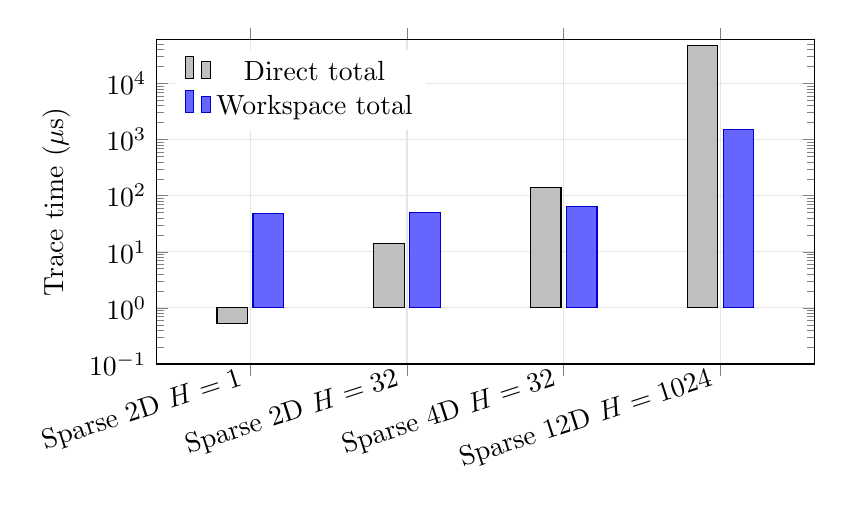
\begin{tikzpicture}
\begin{semilogyaxis}[
 width=.82\linewidth,height=5.7cm,
 ybar,bar width=11pt,enlarge x limits=.2,
 ymin=.1,ymax=60000,
 xtick={1,2,3,4},
 xticklabels={Sparse 2D \(H=1\),Sparse 2D \(H=32\),Sparse 4D \(H=32\),Sparse 12D \(H=1024\)},
 x tick label style={rotate=18,anchor=east},
 ylabel={Trace time (\(\mu\)s)},
 grid=major,grid style={gray!20},
 legend style={at={(.03,.97)},anchor=north west,draw=none,fill=white},
]
\addplot+[fill=gray!50,draw=black,mark=none] coordinates
 {(1,.520) (2,14.050) (3,141.928) (4,48053.051)};
\addplot+[fill=blue!60,draw=blue!80!black,mark=none] coordinates
 {(1,48.194) (2,49.688) (3,64.643) (4,1506.102)};
\legend{Direct total,Workspace total}
\end{semilogyaxis}
\end{tikzpicture}}
\caption{Total costs under the same output contract. Workspace preparation is paid once per trace. In 2D it dominates; in this family it is amortized from 4D and 32 calls. Borrowed outputs are consumed without retention copies. The four workloads do not establish a growth law. Data: \code{perf-workspace-small.csv}.}
\label{fig:workspaceamort}
\end{figure}

\paragraph{Why profile this workspace?}
The preceding campaign indicates \emph{when} reuse helps, but not which functions account for time and allocations. A first PerfChecker profile examines a 7D workspace at $H=32$ to guide code inspection. Sampled stacks cannot by themselves assign a causal fraction of execution time. An initial capture with one operation per profiling window produced no CPU samples~\cite{profilefirst}. The follow-up uses 100 episodes of 256 operations and verifies every output. Its seven warm benchmark observations are separate from those long profiling episodes.

The follow-up completes benchmark, CPU profile, allocation profile, latency, GC, and memory diagnostics. Type information was captured, without an automatic stability verdict, and CPU and allocation stacks were exported. Among 134 CPU samples, 34 stacks include algebra validation and 16 include support validation~\cite{profilesmoke,profilingpreflight}. These are \emph{inclusive} counts: one stack may contain both functions. Under Étendue3D interference, they identify code worth examining but establish neither causal time attribution nor a selection threshold. A separate heap-diagnostic attempt exceeded the temporary disk budget and is not part of these six completed capabilities~\cite{profileheap}.
\FloatBarrier

\subsection{Mask width and the 64/128 boundary}
\paragraph{Why this technique?}
Blade masks let the kernel compute XOR, intersection, and permutation parity with bit operations (Equation~\eqref{eq:blade}). Julia uses \code{UInt64} up to 64 directions, \code{UInt128} through 128, and \code{BigInt} beyond that range. This change targets sparse operands in ambient dimensions 65--128, where dense arrays are impractical but the active mask set can remain small.
\paragraph{Tests, results and limitations.}
The measured improvement belongs to a simplified diagonal kernel compared within one process. At 65D, median coefficient latency falls from 2.129 to 0.179~\(\mu\)s and full-product latency from 86.720 to 4.209~\(\mu\)s; at 128D, coefficient latency falls from 3.179 to 0.204~\(\mu\)s. Boundary tests and 24 paired cases support this finding, but do not establish the same factor for every API. Plans, joins, metrics, and expressions around 64, 128, and 129 dimensions still need matched tests that record actual mask type, allocations, and conversions. Earlier 66D and 128D \code{BigInt} campaigns are from a different revision and cannot be pooled as identical repetitions.

\subsection{Representation of masks from 65 to 128 dimensions}
\paragraph{Why this experiment?}
At 65 dimensions, an \code{UInt64} mask is no longer sufficient; moving immediately to \code{BigInt} can charge an arithmetic and disproportionate allocation for masks still contained in 128 bits. The comparison tests this cost of representation at the border. Since the first scan, the masks use \code{UInt128} between 65 and 128 dimensions. The correction tests cover 63, 64, 65, 70, 127, 128 and 129 dimensions. A second PerfChecker validated 128 cases at borders 63--66 and 127--130, then a paired comparison in the same process validated 24 cases of simplified diagonal core. At 65D, the median of the target coefficient went from 2.129 ~ \(\mu\) s with \code{BigInt} to 0.179 ~ \(\mu\) s with \code{UInt128}; the corresponding whole product went from 86.720 to 4.209 ~ \(\mu\) s and 159\,784 to 8\,816 octets allocated.
At 128D, the pairs are 3.179 / 0.204 ~ \(\mu\) s for the coefficient and 99.299 / 5.671 ~ \(\mu\) s for the entire product. These paired numbers exclude the creation of the support and the first compilation; they are not a gain of the same magnitude demonstrated on all APIs. The \code{BigInt} route remains necessary from 129 dimensions. The protocol, exclusions and complete measurements are included in two accompanying mask-kernel CSV files and archived qualification records.

\begin{figure}[ht]
\centering
\IfFileExists{exploratory_masques.pdf}{\includegraphics[width=.92\linewidth]{exploratory_masques.pdf}}{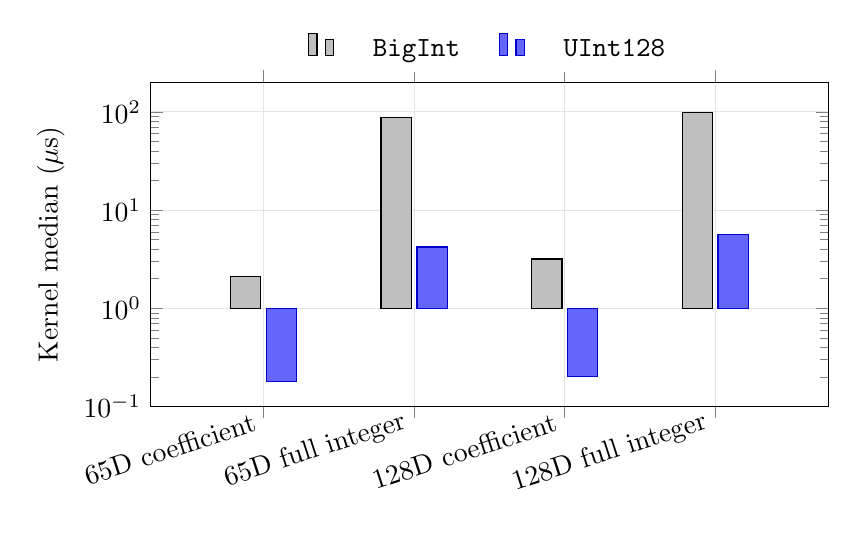
\begin{tikzpicture}
\begin{semilogyaxis}[
 width=.84\linewidth,height=5.7cm,
 ybar,bar width=11pt,enlarge x limits=.25,
 ymin=.1,ymax=200,
 xtick={1,2,3,4},
 xticklabels={65D coefficient,65D full integer,128D coefficient,128D full integer},
 x tick label style={rotate=18,anchor=east},
 ylabel={Kernel median (\(\mu\)s)},
 grid=major,grid style={gray!20},
 legend style={at={(.5,1.03)},anchor=south,legend columns=2,column sep=12pt,draw=none,fill=white},
]
\addplot+[fill=gray!50,draw=black,mark=none] coordinates
 {(1,2.129) (2,86.720) (3,3.179) (4,99.299)};
\addplot+[fill=blue!60,draw=blue!80!black,mark=none] coordinates
 {(1,.179) (2,4.209) (3,.204) (4,5.671)};
\legend{\code{BigInt},\code{UInt128}}
\end{semilogyaxis}
\end{tikzpicture}}
\caption{Two implementations of the \emph{same targeted diagonal kernel}, paired within each dimension. The vertical scale is logarithmic. Support preparation and compilation are excluded, so these are not end-to-end API ratios.}
\label{fig:masques}
\end{figure}
\FloatBarrier

\subsection{Generated code, JIT and native catalogue}
\paragraph{Why this technique?}
As in GAALOP's specialization of geometric-algebra expressions~\cite{gaalop}, known structure can replace dynamic loops and indexing with generated code. The Julia generator unrolls at most 256 paths; a prepared plan remains available when support structures or types are more numerous. Julia compilation has a separate lifecycle from plan construction and data retention~\cite{juliaprecompile}.
\paragraph{Tests, results and limitations.}
Across twelve tested families, 288 prepared and 288 generated outputs match the direct product. A newly compiled 64-path topology can nevertheless cost about 100~ms of JIT; a 256-path topology costs about 440~ms. The 36 strategy choices derived from this corpus are cost-model decisions, not 36 independently timed traces; all choose a prepared plan. In I15.6, a native EGA3 catalog removes JIT from the first known product after restart (Table~\ref{tab:precompile}), but eleven unseen 4D topologies still add 648--658~ms of JIT at \emph{each} restart. One measured catalog build adds 5.47~MiB and 1.67~s. Future tests must separate known and new structures, time full $H$-call episodes in fresh and warm processes, and record cache size, code memory, and the frequency of new topologies.

\subsection{Precompilation and restart}
\paragraph{Why this experiment?}
A fast warm call does not guarantee a fast first response after restarting a process. I15.6 separates catalog creation, object reconstruction, and first compilation of known or previously unseen products. It compares IR and native caches, each with or without an EGA3 precompilation catalog, across 72 fresh processes and 3\,816 phase observations: three restarts for every combination of four cache configurations, two scenarios, and three strategies. Algebras, plans, and buffers are rebuilt in each process, and an independent oracle checks outputs. Table~\ref{tab:precompile} starts timing the first product \emph{after} its objects have been constructed; it includes any compilation of that product but not process startup. Values come from \code{precompile-lifecycle-stages.csv}.

\begin{table}[ht]
\centering\small
\begin{tabular}{@{}lrrr@{}}
\toprule
Configuration & Prepared & Generated & Workspace \\
\midrule
IR, without catalog & 64.875 & 190.480 & 62.885 \\
Native, without catalog & 65.112 & 191.647 & 63.643 \\
IR, with catalog & 59.755 & 143.224 & 59.069 \\
Native, with catalog & 0.008 & 0.122 & 0.015 \\
\bottomrule
\end{tabular}
\caption{First EGA3 product after object reconstruction: median across three fresh processes, in milliseconds.}
\label{tab:precompile}
\end{table}

With a native catalog, the first known product records zero JIT time in all nine relevant processes. Initial \emph{workspace construction} still incurs 2.63--2.77~ms of JIT, so product latency must be distinguished from structural preparation. End-to-end time from launch to the first known result, including the harness, falls from about 2.7--2.9~s without a native catalog to 1.17--1.19~s with one. Only one cache build was measured per configuration; the native catalog adds 5.47~MiB and about 1.67~s to that build, so no amortization threshold follows.

Each session discovers twelve 4D contexts with distinct generated topologies but one plan type. After the first context, the other eleven add 648--658~ms of JIT for the generated route at \emph{each} restart, and none for the prepared-plan and workspace routes. Disk-cache fingerprints remain unchanged across the 72 processes: JIT for these new topologies is not automatically persisted there. The protocol does not test a system image, serialized plans, or an exhaustive catalog. Phase data, sizes, and exclusions appear in the I15.6 CSV files.
\FloatBarrier

\subsection{Long traces and generation}
\paragraph{Why this experiment?}
One product does not represent a session that repeatedly evaluates expressions with stable or changing supports. This campaign therefore measures total cost across several reuse horizons, including preparation and generation, to see which strategies actually amortize their setup. It runs 1, 32, 1\,024, or 10\,000 iterations of $(ab)c$ on sparse supports in dimensions 66 and 128, with stable, alternating, or phased support patterns. It predates the \code{UInt128} switch for 65--128D and describes a different code revision. Coefficients change every iteration; plans are prepared when a context first appears; an independent integer oracle checks every scalar output.

For 10\,000 stable 66D outputs, warm trace times including lazy preparation are 1\,477~ms direct, 66.9~ms with plans, 89.7~ms generated, 101.1~ms with \code{join3}, and 27.9~ms with workspaces. At $H=1$, \code{join3} takes 0.047--0.055~ms depending on the trace, versus 1.13--1.68~ms to construct a workspace. The 10\,000-call traces retain only \emph{one} sample, and this campaign partly overlapped other CPU use. They are screening observations without a reliable dispersion estimate. The repository report \code{perf/long\_horizon\_results/README.md} and CSV files retain cold costs, compilation, allocations, and object graphs. Coefficients change between calls, but one output is not fed into the next; these traces do not test error propagation in a time recurrence.

A separate study of twelve families observes that compiling a new 64-path topology can cost about 100~ms and a 256-path topology about 440~ms. All 288 prepared and 288 generated outputs matched the direct product in tested cases. For these APIs and this corpus, 36 decisions modeled on a training subset at three reuse horizons all selected the prepared plan; their total cost was modeled, not measured through another trace. Distinct supports can already share generated topology. The protocol and CSV files are under \code{perf/generated\_costs/}; ambient 66D still used \code{BigInt} in that revision. Further program compression needs a more varied corpus, observed JIT sharing, and code-memory measurement. Counting distinct topologies alone is insufficient.
\FloatBarrier

\subsection{Structural cache and eviction policy}
\paragraph{Why this technique?}
The Julia cache keys a \code{ProductPlan} by metric, basis, supports, operation, and budget, with bounded LRU eviction. An experimental randomized policy gives an item with $h$ hits eviction weight $1/(1+h)$; it changes cache retention, not algebraic contributions. TinyLFU~\cite{tinylfu} and SIEVE~\cite{sieve} offer other policies in their own domains, without proven Garamon gains. This cache targets recurring structures when callers do not retain plans themselves.
\paragraph{Tests, results and limitations.}
For 40 products with two frequent supports and one intruder, direct execution, LRU, and randomized eviction take 1.60, 2.42, and 1.83~ms; on a scan, they take 1.56, 3.11, and 3.15~ms. A four-phase trace favors both caches, at 1.52, 0.736, and 0.763~ms, whereas abrupt replacement of the frequent supports favors LRU, at 4.09, 1.11, and 4.08~ms, with 76 hits of 80 versus 43 for the recorded random seed~\cite{roadmap}. LRU remains the default explicit cache policy. A replacement decision needs realistic support traces, key and lock costs, retained bytes, hit rate, regeneration cost, and variation across seeds. Caching \emph{computed values} would have a different validity contract from caching structural plans.

\subsection{Factorized forms, active subspaces, and tensor trains}
\paragraph{Why this technique?}
A decomposable blade can remain an exterior product of vectors, a reflection can remain a factor chain, and an active subalgebra can reduce the dimension actually traversed. Tensor trains represent coefficient arrays through successive cores~\cite{oseledets}. For a \emph{diagonal} Clifford product, the Julia construction tracks parity of previously read bits, applies the local factor $(-1)^{a_i p}g_i^{a_i b_i}$, and forms an exact uncompressed train of rank at most $2r_A r_B$. This rank bound belongs to this construction, not to Oseledets's general result. Rank and entry budgets reject oversized expansions. These routes target inputs that are already structured, not arbitrary coefficient arrays.
\paragraph{Tests, results and limitations.}
The 84 tensor-train checks include ranks one and two and dimension 66. With twelve active bits at 66D, each explicit input has 4\,096 coefficients; the result train with its algebra occupies 15\,757 bytes versus about 380\,021 bytes for an explicit input. For a grade-six output, one measured case takes 42.37~\(\mu\)s to construct the train and 6.86~\(\mu\)s to read the product, versus 8\,656.07~\(\mu\)s for an explicit support join~\cite{roadmap}. The comparison begins with \emph{already separable} inputs. Converting arbitrary inputs to low rank may be impossible or more expensive. No approximate truncation or nonorthogonal tensor-train product is validated. A matched future test must include factor/core construction, conversion back to the requested output, attained rank, memory, conditioning, and any ambient-duality constraints.

\subsection{ZDD and change of representation}
\paragraph{Why this technique?}
Zero-suppressed decision diagrams (ZDDs) compress families of sets~\cite{minato}. Active blade masks form a family of subsets of basis directions, so a ZDD may describe a regular support without listing every blade. The current prototype supports only Boolean membership and cardinality, without Clifford coefficients or a weighted product. Matrix representations and changes to an active subspace remain hypotheses: conversion cost, conditioning, and restoration of outputs in the original basis may erase any gain.
\paragraph{Tests, results and limitations.}
For 10\,626 grade-four masks in 24D, a regular support forms 84 ZDD nodes occupying 3\,272 bytes, versus 15\,138 nodes and 659\,216 bytes for an equally large random support. Construction takes 5.44 and 17.65~ms respectively~\cite{roadmap}. This compares \emph{support formats}, not products. A product experiment would need coefficients, exact join or accumulation on the diagram, matched dictionary/list/block baselines, and conversion in total time. Irregular supports provide an essential negative case.

\subsection{Approximate pruning, residues and replay}
\paragraph{Why this technique?}
A contribution can be omitted under a threshold, or accepted with a probability and reweighted; a residue log can then correct an output, or a segment is replayed from an exact state. Rhee and Glynn~\cite{rhee} random correcting estimators motivate the question of bias, without guaranteeing the accuracy of a non-linear trajectory. These methods require an \emph{explicit approximation mode} and an error rule; they are not hidden routes of the exact product.
\paragraph{Tests, results and limitations.}
The 2\,700-case prototype still forms every candidate contribution, so it does not demonstrate savings from avoiding path generation. The contribution threshold has a median time ratio of 0.817 in bilinear recurrences, with error, but 1.017 in affine recurrences. Carrying a residual restores all 540 final rational outputs examined, at median time ratios of 1.149 and 1.433 for bilinear and affine recurrences, but matches the \code{Float64} output bit for bit in only 279 cases. Exact segment replay matches all 540 floating-point controls bit for bit, at ratios of 1.140 and 1.198 (Table~\ref{tab:pruning}). An unbiased Bernoulli decision at one step does not bound rare errors after repeated steps. A useful next experiment would reject whole blocks \emph{before forming} contributions through certified bounds, then measure the error tail, certification and correction costs over longer horizons against an exact oracle for the same output.

\subsection{Approximate pruning in recurrences: Exploratory result}
\paragraph{Why this experiment?}
Omitting small contributions may reduce work, but their effects propagate through a recurrence. This experiment compares the cost and error of pruning with the cost of restoring an exact trajectory. A prototype under \code{perf/}, separate from the exact public kernel, validates 2\,700 cases and rejects another 540 cases before execution. Validation here means that each method satisfies its protocol assertions; it does not imply that approximate outputs are accurate. The cases span twelve dimensions from 2 to 128, at most four active directions, three metric classes, affine and bilinear recurrences, and seven timing samples per case. The large ambient dimensions do not expand the arithmetic beyond those four active directions. Every method still forms each candidate contribution; the methods differ in how they update or correct outputs.

\begin{table}[ht]
\centering\small
\begin{tabular}{@{}lrr@{}}
\toprule
Method & Median affine ratio & Median bilinear ratio \\
\midrule
Contribution threshold & 1.017 & 0.817 \\
Bernoulli roulette ($p=1/2$) & 1.115 & 0.904 \\
Carried and corrected residual & 1.433 & 1.149 \\
Exact segment replay & 1.198 & 1.140 \\
\bottomrule
\end{tabular}
\caption{Total method time divided by the exact baseline time for the same configuration. Common preparation is excluded and correction is included. Values are medians of paired ratios, not ratios of medians; below one means an observed time saving. Data: \code{perf-pruning-recurrences.csv}.}
\label{tab:pruning}
\end{table}

For bilinear recurrences, the threshold reduces median time by 18.3\% in this protocol but introduces error. The residual restores the exact rational final output in 540 configurations yet matches only 279 floating-point outputs bit for bit. Replay matches all 540 floating-point outputs bit for bit, at a higher median cost. Bernoulli roulette with probability $1/2$ is conditionally unbiased for one step but can produce rare trajectories with very large error; 32 seeds per configuration do not characterize that tail. No measured result shows a gain from pruning within \code{ProductWorkspace}, or an exact route faster than the baseline. The archived pruning campaign records the oracles, horizons, intermediate errors, and limits of this first experiment.
\FloatBarrier

\subsection{Contextual selector and hyperparameter tuning}
\paragraph{Why this technique?}
SATzilla~\cite{satzilla}, ASlib~\cite{aslib}, and AutoFolio~\cite{autofolio} provide methods for selecting and configuring algorithms. Before a Garamon product is evaluated, a selector can inspect dimension, mask type, metric, support sizes and grades, requested outputs, expected reuse horizon, and the availability of a compatible plan or workspace. It may choose only an admissible exact strategy. Feature extraction, inference, validation, and fallback all have costs. SHAP~\cite{shap} may explain a trained model's predictions, but cannot by itself establish causality or speedup.
\paragraph{First prototype and measurement.}
An analytical, untrained rule now chooses among five exact routes for requested coefficients of $(ab)c$; its weights are assumptions rather than learned times~\cite{selectionreport}. It passes 402/402 targeted tests. A one-thread PerfChecker smoke test in Euclidean EGA4, for one scalar coefficient and $H=1$, qualifies six routes: five forced choices and the automatic choice. Fifteen observations per route give 90 samples. The warm episode includes feature extraction, selection, preparation, and an independently owned output. The rule selects \code{join3}, with a median of 60.135~\(\mu\)s versus 59.466~\(\mu\)s for the same forced route. Because Étendue3D was active, the 0.669~\(\mu\)s difference cannot be assigned to routing alone. First-compilation probes are diagnostic and are excluded from these warm medians.

The prepared matrix contains 144 structures and 5\,184 replay identities, but only eight independent training groups remain after leakage control, below the declared minimum of twenty. Hyperparameter tuning, regret on held-out families, routing thresholds, and general gains therefore remain unvalidated. Earlier targeted triple-product and complete binary-product campaigns use different contracts and cannot supply comparable training labels. The fixed protocol~\cite{selectionprotocol} uses the same expression $(ab)c$, one or four independently owned outputs, reuse horizons $H=1,32,1\,024$, and five exact candidates: complete, recursive, \code{join3}, prepared, and workspace. Each qualifying episode must separate admission, preparation, first JIT, execution, reconstruction after cancellation, and copying. Algebra families and support families are kept disjoint across training, validation, and testing; renamed versions of one support stay in the same group. Baselines are direct execution, the best fixed choice, and the analytical rule. A small decision tree or regularized cost model may use at most twelve configurations selected on validation data. A future result must report total time, memory, rejected cases, and regret relative to the best retrospectively measured route, including the tail of losses. That retrospective oracle is not an executable policy available for free.

\subsection{Threads, processes, compact batches, and GPU}
\paragraph{Why this technique?}
Independent products can share an immutable plan if each task owns a separate mutable workspace. Julia tasks can migrate between threads, so simply indexing a buffer by thread number does not ensure exclusive access~\cite{juliathreads}. Separate processes add startup, serialization, and state duplication. GPU comparison requires an implemented kernel, compact data, a matched output contract, and timing that includes transfers, synchronization, and launch~\cite{cudaperf}.
\paragraph{Current test and proposed experiment.}
For 32 repeated products of the \emph{same objects} in 12D, the implemented \code{PackedProductBatch} takes 39.93~\(\mu\)s in total versus 71.62~\(\mu\)s for the ordinary prepared batch. For 32 distinct objects with the same support, it loses: 586.06 versus 72.62~\(\mu\)s~\cite{roadmap}. This contrast exposes conversion costs. A separate CPU protocol~\cite{parallelprotocol} proposes 1--16 threads and 1--8 processes on independent batches, with the same oracle and owned outputs, while separating startup, JIT, copying, serialization, and memory. A later four-thread packed-product pilot is reported below; other thread counts and process speedups remain unvalidated.

\paragraph{Packed CUDA.jl pilot: why test it?}
Packing many products with a shared path plan gives the GPU contiguous coefficient matrices and independent output columns. The pilot asks when enough products repay transfers, device setup, and a copied host result. It uses Garamon.jl's \code{run\_packed\_batch} on the CPU and, on the GPU, the \emph{same} plan and packed operands. GPU paths are grouped by output coefficient while preserving contribution order within each coefficient; one thread computes an output-column pair, without atomics or pruning. Both routes return a new, independently owned dense \code{Float64} matrix on the host. A separately timed device-only route that reuses an output buffer is diagnostic and has no matched owned-output CPU comparator. Every timed GPU call synchronizes before returning. Thus the complete episode includes plan creation, packing, GPU transfers, kernel, synchronization, and host copy~\cite{gpupacked}.

\emph{Correctness and paired experiment.} With CUDA.jl 6.4.0 and Julia 1.13 on a GeForce RTX 3060 Ti, the targeted suite passes 1\,690\,575/1\,690\,575 assertions under forced bounds checks and again under automatic checks. It compares GPU, packed CPU, and an independent integer oracle on exactly representable \code{Float64} coefficients across dimensions 2, 8, 65, and 128, two support families, positive, mixed, and degenerate signatures, and horizons 1, 32, and 1\,024. This establishes the tested coefficient and ownership contract, not bitwise identity for arbitrary floating inputs. A qualified 8D/65D smoke test has 24/24 cases and 588 observations. The larger paired screen qualifies 384/384 cases and 9\,408 observations across twelve dimensions, two support families, horizons $H=1,32,1\,024,8\,192$, and two route orders. The timed grid uses a positive metric. Each complete episode is measured directly rather than assembled from phase medians. Figure~\ref{fig:gpupacked} counts pairs where the GPU has the lower median, with the same host-output contract on both routes~\cite{gpupacked}.

\begin{figure}[ht]
\centering
\IfFileExists{exploratory_gpupacked.pdf}{\includegraphics[width=.92\linewidth]{exploratory_gpupacked.pdf}}{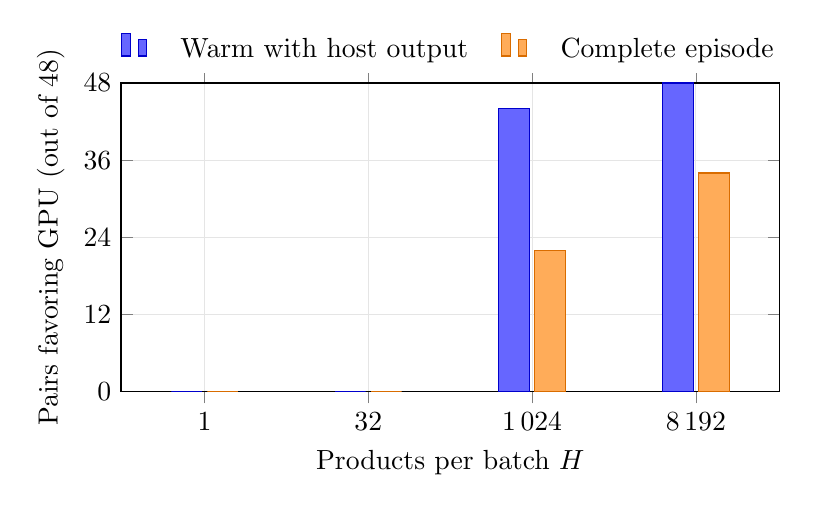
\begin{tikzpicture}
\begin{axis}[
 width=.82\linewidth,height=5.5cm,
 ybar,bar width=11pt,enlarge x limits=.17,
 ymin=0,ymax=48,ytick={0,12,24,36,48},
 xtick={1,2,3,4},xticklabels={1,32,1\,024,8\,192},
 xlabel={Products per batch \(H\)},
 ylabel={Pairs favoring GPU (out of 48)},
 grid=major,grid style={gray!20},
 legend style={at={(.5,1.03)},anchor=south,legend columns=2,column sep=10pt,draw=none,fill=white},
]
\addplot+[fill=blue!60,draw=blue!80!black,mark=none] coordinates
 {(1,0) (2,0) (3,44) (4,48)};
\addplot+[fill=orange!65,draw=orange!85!black,mark=none] coordinates
 {(1,0) (2,0) (3,22) (4,34)};
\legend{Warm with host output,Complete episode}
\end{axis}
\end{tikzpicture}}
\caption{Paired packed GPU wins over CPU with the same owned host output. Warm execution starts with prepared resident inputs; complete episodes include packing, transfers, synchronization, and host output. Median CPU/GPU ratios for complete episodes are 0.457, 0.581, 0.986, and 1.027 at the four horizons. A warm win does not imply a total-episode win~\cite{gpupacked}.}
\label{fig:gpupacked}
\end{figure}
\FloatBarrier

At $H=1$ and $H=32$, the GPU loses all 48 paired complete episodes at each horizon. At $H=1\,024$, it wins 22/48 although warm computation with host return wins 44/48; the median complete-episode CPU/GPU ratio is 0.986. At $H=8\,192$, warm computation wins 48/48, but complete episodes win 34/48 with median ratio 1.027. The ratios are medians of 48 within-pair ratios, not ratios of pooled times. Construction favors the GPU in zero pairs at $H=8\,192$; transfers and setup nearly erase its warm advantage. The GPU's diagnostic reused-device-output time cannot replace these owned-host-output measurements. BenchmarkTools reports CPU allocations, not VRAM allocations; the measured free-VRAM change is only a before/after snapshot, not a per-case peak. The campaign's operator status \code{isolated} records no other declared user computation, yet the GPU drove the display and showed nonzero initial use. This is not certified hardware isolation. No dimension-only threshold, automatic GPU route, or paired upstream C++ comparison follows. Mixed and degenerate metrics are validated for correctness but not timed in this grid; device-resident downstream outputs and denser workloads need separate measurement~\cite{gpupacked}.

\paragraph{Where does the GPU time go?}
A distinct CUPTI profile probes \emph{higher-rank} support at $H=8\,192$ in 8D and 65D, with the same packed plan and independent integer oracle before and after tracing. It separates a reused device output, a fresh host output from resident inputs, and a complete episode. Figure~\ref{fig:gpu-copy-profile} shows the kernel and device-to-host copy within the resident-input trace. The copied outputs contain about 5.5 and 14~MiB; complete episodes additionally transfer both packed operands and plan paths to the GPU. These instrumented phase durations explain why a fast kernel need not make the host-output API fast. CUPTI tracing changes timing and includes unclassified host activity, so the plotted durations must \emph{not} be compared with PerfChecker medians~\cite{gpupacked}.

\begin{figure}[ht]
\centering
\IfFileExists{exploratory_gpu-copy-profile.pdf}{\includegraphics[width=.92\linewidth]{exploratory_gpu-copy-profile.pdf}}{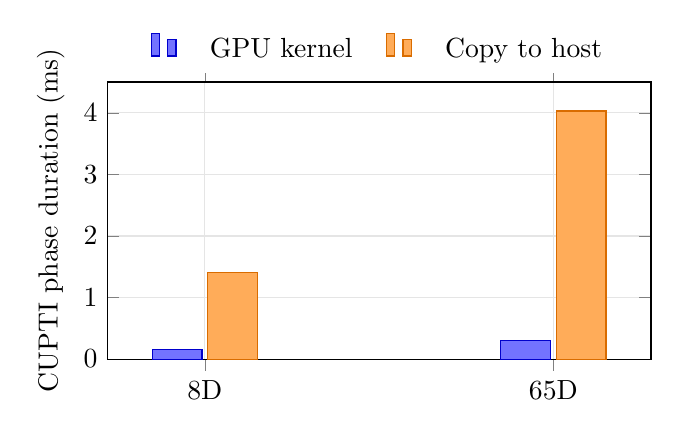
\begin{tikzpicture}
\begin{axis}[
 width=.7\linewidth,height=5.1cm,
 ybar,bar width=18pt,enlarge x limits=.28,
 ymin=0,ymax=4.5,ytick={0,1,2,3,4},
 xtick={1,2},xticklabels={8D,65D},
 ylabel={CUPTI phase duration (ms)},
 grid=major,grid style={gray!20},
 legend style={at={(.5,1.03)},anchor=south,legend columns=2,column sep=10pt,draw=none,fill=white},
]
\addplot+[fill=blue!55,draw=blue!80!black,mark=none] coordinates {(1,.159) (2,.299)};
\addplot+[fill=orange!65,draw=orange!85!black,mark=none] coordinates {(1,1.40) (2,4.03)};
\legend{GPU kernel,Copy to host}
\end{axis}
\end{tikzpicture}}
\caption{Diagnostic CUPTI trace at $H=8\,192$: copy/kernel ratios are about 8.8 in 8D and 13.5 in 65D. Instrumentation prevents comparison with unprofiled episode medians~\cite{gpupacked}.}
\label{fig:gpu-copy-profile}
\end{figure}
\FloatBarrier

\paragraph{Does a pinned host output remove the copy cost?}
Pinned host memory may accelerate a device-to-host copy, but a new independently owned \code{Matrix\{Float64\}} must be allocated and registered on \emph{every} call. The experimental route pins that new matrix, copies into it, synchronizes, and keeps the registration for the output's lifetime. It retains the same ordered packed kernel, paths, support, and oracle as ordinary GPU output and packed CPU output. A 512~MiB per-output admission budget does not bound the total pinned RAM if an application holds many results. Targeted tests pass 361/361 assertions under forced bounds checks and again under automatic checks, including distinct ownership, exact results, and budget refusals across 8D/65D and positive, mixed, and degenerate signatures~\cite{gpupinned}.

The first paired screen qualifies 72/72 cases and 1\,512 observations in 8D/65D. At $H=8\,192$, pinning wins all 6/6 complete-episode pairs against ordinary GPU output, with median ordinary/pinned ratio 1.035. That small screen motivated an extension, not a default route. The twelve-dimension, two-support-family screen qualifies 432/432 cases and 9\,072 observations, with three balanced route orders and positive-metric timing. At $H=1\,024$, pinning loses all 72/72 complete-episode pairs to ordinary GPU output (median ordinary/pinned ratio 0.832). At $H=8\,192$, it wins only 30/72 (median ratio 0.995). Within that long horizon, \code{low\_rank\_high\_grade} wins 7/36 pairs (median 0.987), while \code{higher\_rank} wins 23/36 (median 1.051). Figure~\ref{fig:gpu-pinned} makes the dependence on corpus and support visible. The ratios compare directly timed complete episodes, including registration and fresh host output; a copy-only profile cannot predict them~\cite{gpupinned}.

\begin{figure}[!htbp]
\centering
\IfFileExists{exploratory_gpu-pinned.pdf}{\includegraphics[width=.92\linewidth]{exploratory_gpu-pinned.pdf}}{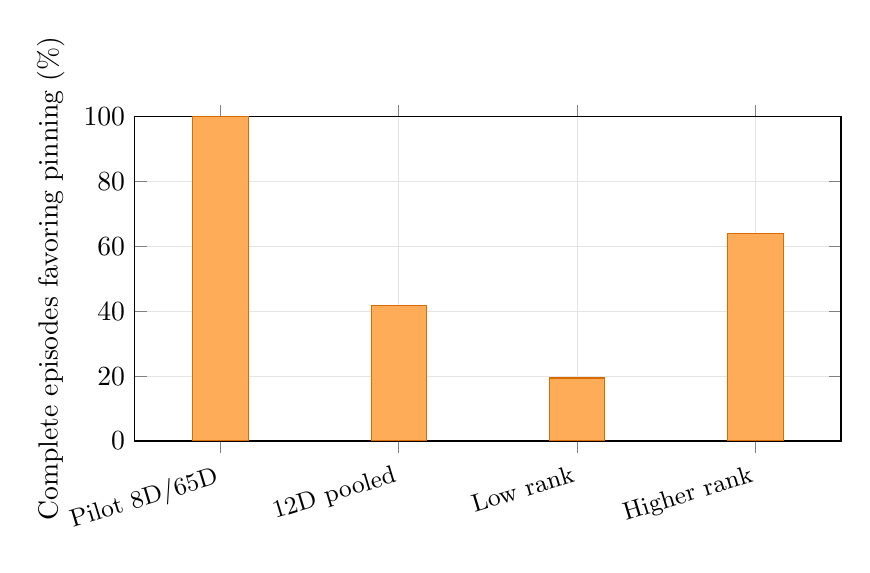
\begin{tikzpicture}
\begin{axis}[
 width=.87\linewidth,height=5.7cm,
 ybar,bar width=20pt,enlarge x limits=.16,
 ymin=0,ymax=100,ytick={0,20,40,60,80,100},
 xtick={1,2,3,4},
 xticklabels={Pilot 8D/65D,12D pooled,Low rank, Higher rank},
 x tick label style={rotate=17,anchor=north east,font=\small},
 ylabel={Complete episodes favoring pinning (\%)},
 grid=major,grid style={gray!20},
]
\addplot+[fill=orange!65,draw=orange!85!black,mark=none] coordinates
 {(1,100) (2,41.67) (3,19.44) (4,63.89)};
\end{axis}
\end{tikzpicture}}
\caption{Pinned versus ordinary GPU output at $H=8\,192$: 6/6 wins in the two-dimension pilot, then 30/72 in the twelve-dimension screen, split into 7/36 \code{low\_rank\_high\_grade} and 23/36 \code{higher\_rank}. The small pilot sampled only a limited support/dimension set. At $H=1\,024$ in the larger screen, pinning wins 0/72~\cite{gpupinned}.}
\label{fig:gpu-pinned}
\end{figure}
\FloatBarrier

The pinned route beats the CPU in 51/72 complete episodes at $H=8\,192$, yet the ordinary GPU route often beats it within the same campaign. BenchmarkTools allocation bytes do not reveal how long host pages remain pinned or the peak VRAM use. The operator-declared \code{isolated} status excludes other declared user computation but not display activity (21\% GPU use before the broad screen). Pinning therefore remains an explicit experimental option; no automatic threshold follows from dimension or batch size alone. A future test needs a real device-resident consumer, measured registration and memory lifetime, and repeated runs with monitored GPU activity~\cite{gpupinned}.

\paragraph{Does a four-thread CPU change the GPU crossover?}
The earlier packed CPU/GPU comparison uses a sequential CPU baseline. A new pilot keeps the \emph{same} packed plan, ordered paths, \code{Float64} coefficients, supports, and independently owned host output while adding a four-thread Julia CPU route. A static scheduler assigns disjoint output columns to the four threads; each column preserves the sequential contribution order. The GPU uses the same plan and returns a new host matrix. This tests whether the GPU advantage survives a stronger CPU baseline without changing the arithmetic task. The targeted suite passes 1\,690\,504/1\,690\,504 exact assertions under forced bounds checks and again under automatic checks, across 2D/8D/65D/128D, two support families, three metric signatures, and $H=1,32,1\,024$. An independent integer oracle checks every coefficient; separate checks verify ownership of successive outputs~\cite{cpu4gpu}.

A first 8D/65D \code{higher\_rank} screen qualifies 72/72 cases and 1\,512 observations. Its six long-horizon pairs favor the GPU over the sequential CPU in all 6/6 complete episodes, but favor the four-thread CPU over the GPU in all 6/6. The broader screen qualifies 432/432 cases and 9\,072 observations over twelve dimensions, two support families, $H=1\,024,8\,192$, three routes, and three balanced orders. It times construction, warm execution with a fresh output, and complete episodes \emph{directly}, with seven observations per phase. Speed measurements use a positive metric; mixed and degenerate signatures occur in the exactness suite only. Figure~\ref{fig:cpu4gpu} reports complete-episode paired wins in this broader campaign, with 72 dimension/family/order pairs per horizon~\cite{cpu4gpu}.

\begin{figure}[!htbp]
\centering
\IfFileExists{exploratory_cpu4gpu.pdf}{\includegraphics[width=.92\linewidth]{exploratory_cpu4gpu.pdf}}{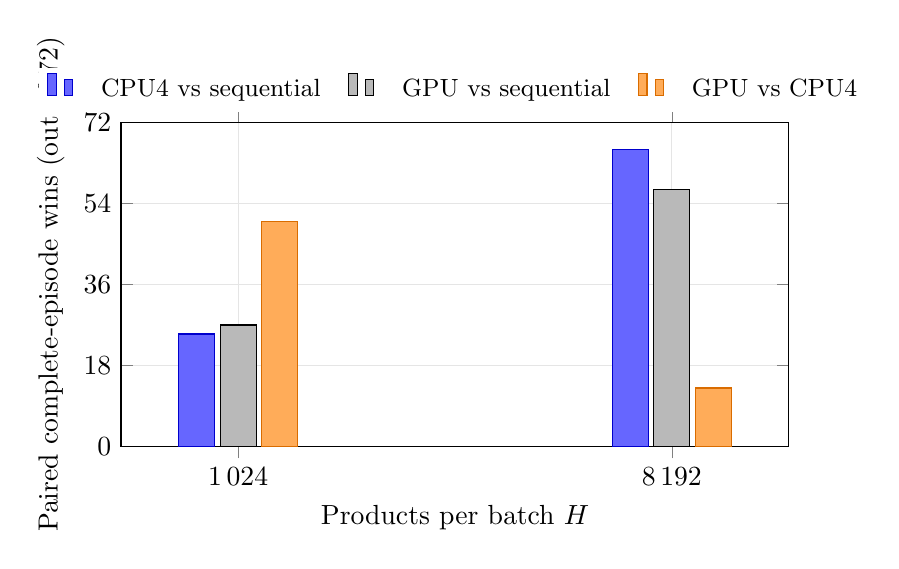
\begin{tikzpicture}
\begin{axis}[
 width=.83\linewidth,height=5.7cm,
 ybar,bar width=13pt,enlarge x limits=.27,
 ymin=0,ymax=72,ytick={0,18,36,54,72},
 xtick={1,2},xticklabels={1\,024,8\,192},
 xlabel={Products per batch \(H\)},
 ylabel={Paired complete-episode wins (out of 72)},
 grid=major,grid style={gray!20},
 legend style={at={(.5,1.03)},anchor=south,legend columns=3,column sep=8pt,draw=none,fill=white,font=\small},
]
\addplot+[fill=blue!60,draw=blue!80!black,mark=none] coordinates {(1,25) (2,66)};
\addplot+[fill=gray!55,draw=black,mark=none] coordinates {(1,27) (2,57)};
\addplot+[fill=orange!65,draw=orange!85!black,mark=none] coordinates {(1,50) (2,13)};
\legend{CPU4 vs sequential,GPU vs sequential,GPU vs CPU4}
\end{axis}
\end{tikzpicture}}
\caption{Paired complete episodes with identical packed arithmetic and new owned host outputs. At $H=8\,192$, GPU wins 57/72 against sequential CPU but only 13/72 against CPU4; the median CPU4/GPU ratio is 0.970 (below one favors CPU4). At $H=1\,024$, GPU wins 50/72 against CPU4, median ratio 1.064~\cite{cpu4gpu}.}
\label{fig:cpu4gpu}
\end{figure}
\FloatBarrier

All 72 warm four-thread calculations beat the sequential CPU at each measured horizon, with median sequential/CPU4 ratios 2.040 at $H=1\,024$ and 2.158 at $H=8\,192$. Yet at $H=1\,024$ only 25/72 \emph{complete} episodes favor CPU4 (median ratio 0.871), because plan construction, packing, and scheduling dominate many short or low-path cases. At $H=8\,192$, CPU4 wins 66/72 episodes against sequential CPU and 59/72 against GPU. The GPU beats CPU4 in 49/72 warm computations but only 13/72 complete episodes: packing, transfers, and host return can reverse the warm ranking. Support matters as well: at $H=1\,024$, CPU4 wins only 1/36 complete episodes against sequential CPU for \code{low\_rank\_high\_grade}, versus 24/36 for \code{higher\_rank}; at $H=8\,192$, CPU4 beats GPU in 34/36 higher-rank episodes. Ratios describe medians of within-pair ratios, not pooled timings, and the small pilot and broad screen remain separate archives. The operator-declared \code{isolated} status records no other user computation, not reserved CPU cores or an idle display GPU (24\% use before the broad screen). No dimension-only threshold follows. Other CPU thread counts, scheduling and frequency control, mixed/degenerate speed cases, and a real device-resident output consumer remain to be tested~\cite{cpu4gpu}.

\paragraph{What changes when four operand sets remain resident?}
The preceding GPU pilots return an independently owned host matrix \emph{after every product}. A different long-use contract packs four operand sets once, alternates among them for $R$ products across $H$ columns, and sums \emph{every} product contribution into one final matrix. The GPU keeps those operands and the partial sum on device, queues the $R$ ordered kernels in one stream, synchronizes, and copies a single independently owned \code{Float64} matrix to the host. Sequential CPU and four-thread CPU accumulate the same ordered paths into their own new host matrices; the four-thread route assigns independent columns to disjoint workers. Thus this is an exact sum with more arithmetic as $R$ grows, not pruning or a device-only output. It has the same plan and four packed inputs on all three routes, but a \emph{different output contract} from the per-product-host-output campaigns~\cite{residentsum}.

\emph{Why measure both warm and complete time?} Construction builds the plan and four packed sets, uploading them for the GPU. The warm phase starts with resident inputs yet still computes the full sum and returns \emph{one fresh host output}. The complete episode directly times construction, all $R$ products, synchronization, and that final host result. Neither the warm phase nor a reused device-output kernel can stand in for the complete episode. A combined 512~MiB admission budget covers the four resident workspaces per route; CUDA pool and compilation buffers require separate memory observation. Exactness tests pass 5\,860\,444/5\,860\,444 assertions under forced bounds checks and again under automatic checks. An independent integer oracle verifies every sum coefficient and distinct output ownership across 8D/65D, two supports, three signatures, $H=1,32,1\,024$, and $R=1,4,16$. Mixed and degenerate signatures are correctness cases; timed grids use a positive metric~\cite{residentsum}.

A two-dimension pilot qualifies 108/108 cases and 2\,268 observations. The separate twelve-dimension screen qualifies 648/648 cases and 13\,608 observations across dimensions 2--128, both support families, three route orders, and the $(H,R)$ workloads $(32,32)$, $(1\,024,8)$, and $(1\,024,32)$. Each of CPU1, CPU4, and GPU has seven observations per phase; all 648 outputs pass the independent oracle. Figure~\ref{fig:resident-sum} counts GPU wins over CPU4 in \emph{directly measured complete episodes}, 72 paired dimension/family/order comparisons per workload. The CPU4/GPU ratio is the median of 72 within-pair median ratios; above one favors GPU. It is not a confidence interval or a ratio of pooled times~\cite{residentsum}.

\begin{figure}[!htbp]
\centering
\IfFileExists{exploratory_resident-sum.pdf}{\includegraphics[width=.92\linewidth]{exploratory_resident-sum.pdf}}{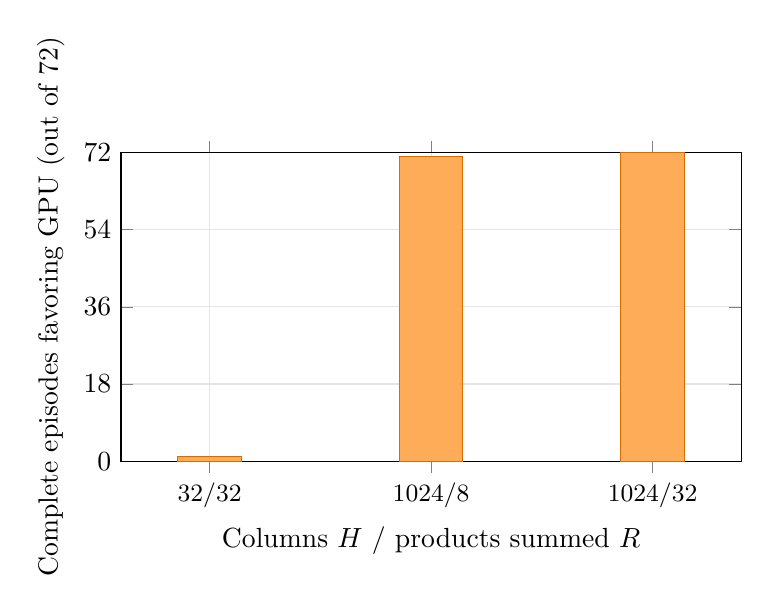
\begin{tikzpicture}
\begin{axis}[
 width=.78\linewidth,height=5.5cm,
 ybar,bar width=23pt,enlarge x limits=.20,
 ymin=0,ymax=72,ytick={0,18,36,54,72},
 xtick={1,2,3},xticklabels={32/32,1024/8,1024/32},
 x tick label style={font=\small},
 xlabel={Columns $H$ / products summed $R$},
 ylabel={Complete episodes favoring GPU (out of 72)},
 grid=major,grid style={gray!20},
]
\addplot+[fill=orange!65,draw=orange!85!black,mark=none] coordinates
 {(1,1) (2,71) (3,72)};
\end{axis}
\end{tikzpicture}}
\caption{Exact final-sum contract with four reused packed operand sets and one owned host output. GPU wins over CPU4 are 1/72, 71/72, and 72/72; median CPU4/GPU complete-episode ratios are 0.565, 1.072, and 1.199, respectively. These figures do not measure the per-product host-output API~\cite{residentsum}.}
\label{fig:resident-sum}
\end{figure}
\FloatBarrier

At $H=1\,024,R=32$, all 24 dimension/support fixtures favor GPU in all three orders. The median CPU4/GPU ratio is 1.179 for \code{low\_rank\_high\_grade} and 1.947 for \code{higher\_rank}; the support changes the gain even at the same dimension and horizon. At $H=1\,024,R=8$, 71/72 complete episodes favor GPU, but only 68/72 warm calculations do. At $H=32,R=32$, GPU wins only 1/72 complete episodes and no warm comparisons: launches and preparation remain costly for narrow batches. The GPU beats sequential CPU in 72/72 episodes at $H=1\,024,R=32$, with median CPU1/GPU ratio 1.728; that baseline does not replace CPU4. The largest recorded first-call compilation takes 1.245~s, outside these episode medians. Peak process RSS was 2.08~GB under the 4~GB cap, whereas CPU allocation counts do not measure peak VRAM. The GPU drove the display (24\% utilization before, 3\% after); \code{isolated} records only no other declared user computation. These data suggest an explicit resident-sum option for long reuse, not an automatic threshold. Future work must measure VRAM peaks and data lifetime, more resident-set counts and CPU thread counts, cold episodes, and a downstream computation that reuses the output on GPU. The upstream C++ generator has no matched resident-sum route, so this campaign makes no C++ speed comparison~\cite{residentsum}.

\paragraph{Can one exact kernel fuse the $R$ resident products?}
The resident-sum GPU route above submits $R$ kernels in one stream, retaining the four packed input sets and partial sum on device before returning one final host matrix. An experimental alternative in \code{perf/} executes the same $R$ products \emph{inside one kernel}: each thread owns one final output coefficient, cycles through the same four inputs, preserves path and addition order, and writes that coefficient once. No contribution is removed, and the final independently owned host output is unchanged. Fewer launches and partial-sum memory round trips motivate fusion; register pressure and reduced parallelism may offset them. The separate CUDA Graph pilot below reuses a captured sequence of $R$ kernels; it does not fuse them, and this fusion campaign performs no graph capture~\cite{residentfusion}.

The targeted Julia 1.13 suite passes 8\,790\,773/8\,790\,773 assertions under forced bounds checks and again under automatic checks. It compares the fused kernel with an independent \code{Int64} oracle, CPU1, CPU4, and the $R$-kernel GPU route on 8D/65D, two support families, positive, mixed, and degenerate metrics, $H=1,32,1\,024$, and $R=1,4,16$. A 512~MiB resident-space budget and invalid-request refusals are checked. The two-dimensional pilot qualifies 108/108 cases and 2\,268 observations. The separate twelve-dimensional screen qualifies 648/648 cases and 13\,608 observations across two families, three balanced route orders, and $(H,R)=(32,32),(1\,024,8),(1\,024,32)$. Its three \emph{paired} routes are CPU4, $R$-kernel GPU, and fused GPU; sequential CPU is absent from this duel. Each case has seven measurements each of construction, warm resident-input computation with one fresh host output, and the directly timed complete episode. As before, warm time is not a substitute for preparation, synchronization, and final host return~\cite{residentfusion}.

\begin{figure}[!htbp]
\centering
\IfFileExists{exploratory_resident-fusion.pdf}{\includegraphics[width=.92\linewidth]{exploratory_resident-fusion.pdf}}{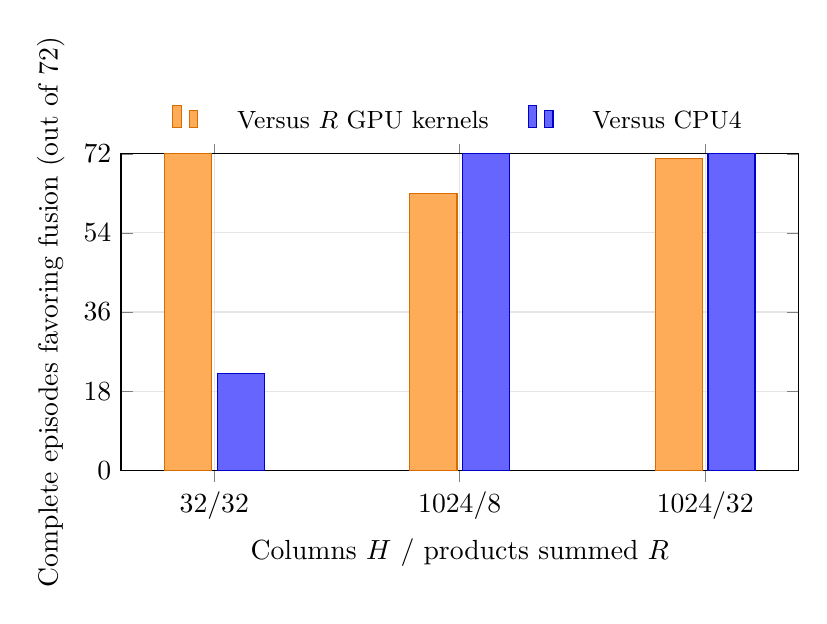
\begin{tikzpicture}
\begin{axis}[
 width=.84\linewidth,height=5.6cm,
 ybar,bar width=17pt,enlarge x limits=.19,
 ymin=0,ymax=72,ytick={0,18,36,54,72},
 xtick={1,2,3},xticklabels={32/32,1024/8,1024/32},
 xlabel={Columns $H$ / products summed $R$},
 ylabel={Complete episodes favoring fusion (out of 72)},
 grid=major,grid style={gray!20},
 legend style={at={(.5,1.03)},anchor=south,legend columns=2,column sep=12pt,draw=none,fill=white,font=\small},
]
\addplot+[fill=orange!65,draw=orange!85!black,mark=none] coordinates {(1,72) (2,63) (3,71)};
\addplot+[fill=blue!60,draw=blue!80!black,mark=none] coordinates {(1,22) (2,72) (3,72)};
\legend{Versus $R$ GPU kernels,Versus CPU4}
\end{axis}
\end{tikzpicture}}
\caption{Fused resident sum against the two matched alternatives in the twelve-dimensional screen. Median old-GPU/fused ratios are 1.472, 1.030, and 1.093; median CPU4/fused ratios are 0.870, 1.100, and 1.299. Above one favors fusion. All bars use the same single final owned host output~\cite{residentfusion}.}
\label{fig:resident-fusion}
\end{figure}
\FloatBarrier

At $H=32,R=32$, fusion wins 72/72 complete episodes against the $R$-kernel GPU (median ratio 1.472), yet only 22/72 against CPU4 (median ratio 0.870). Removing launches does not erase the CPU advantage in most narrow-batch fixtures. At $H=1\,024,R=8$, it wins 63/72 against the prior GPU (1.030) and 72/72 against CPU4 (1.100). At $H=1\,024,R=32$, it wins 71/72 against the prior GPU (1.093) and 72/72 against CPU4 (1.299). The low-rank and higher-rank median old-GPU/fused ratios at that last workload are 1.071 and 1.118; CPU4/fused medians are 1.275 and 2.159. Warm fusion wins 72/72 at $H=32,R=32$ with median old-GPU/fused ratio 2.353, larger than the complete-episode ratio because preparation and final copy remain. These medians summarize within-pair ratios; the two GPU routes and CPU4 are compared only within this new campaign~\cite{residentfusion}.

\emph{Preserved reversal and focused replay.} In the full screen, 12D \code{higher\_rank} at $H=1\,024,R=32$ has one first-order reversal: the $R$-kernel GPU episode takes 3.461~ms versus 4.415~ms for fusion (old/fused ratio 0.784), although warm computation favors fusion. A separate source-unchanged replay qualifies 54/54 cases and 1\,134 observations across that cell and two warm anomalies, using two cycles of three orders. In the disputed cell, fusion wins 6/6 complete episodes and 6/6 warm comparisons; its median old/fused episode ratio is 1.107. The original loss remains part of the full-screen record. Its cause is unknown; the replay does not erase it or establish a fixed effect. The display GPU was active before the broad screen (26\%, versus 3\% after) and before the replay (23\%, versus 3\% after). The operator label \code{isolated} means no other declared user computation, not certified hardware isolation~\cite{residentfusion}.

Fusion remains experimental in \code{perf/}. The paired fusion duel has no sequential-CPU route, and the upstream C++ generator has no matched fused resident sum. No automatic threshold or C++ speed comparison follows. Peak VRAM, first compilation and restarts, resident-set lifetimes, and other CPU thread counts still require measurement. The distinct CUDA Graph pilot below tests repeated sums with the same input values, including capture and instantiation costs~\cite{residentfusion}.

\paragraph{Does a captured CUDA Graph repay its construction?}
Fusion puts $R$ products in one kernel; the CUDA Graph prototype instead captures a reset of the partial sum and the same $R$ ordered GPU kernels, then instantiates that graph once. Four packed operand sets remain resident. Each graph replay synchronizes and returns a \emph{new, independently owned host matrix} containing the exact final sum. The workload repeats the \emph{same input values} for $Q$ separate outputs, deliberately favoring reuse of the captured structure; changing values in the resident buffers is untested. The paired alternatives are CPU4, ordinary $R$-kernel GPU, fused GPU, and graph GPU. All compute the same contributions and return $Q$ owned outputs. The build phase charges resident preparation plus graph capture and instantiation; warm time covers one owned sum, and the complete episode directly charges build plus all $Q$ outputs~\cite{residentgraph}.

Under Julia 1.13, targeted tests pass 5\,854\,756/5\,854\,756 exact assertions with forced bounds checks and again with automatic checks. They cross 8D/65D, two support families, positive/mixed/degenerate signatures, $H=32,1\,024$, and $R=1,8,32$. Two graph replays return distinct host matrices, each matching the independent integer oracle, the $R$-kernel route, and fusion. The qualified PerfChecker pilot has 192/192 cases and 4\,032 observations across four balanced route orders and three workloads: $(H,R,Q)=(32,32,32),(1\,024,8,32),(1\,024,32,8)$. Its two dimensions and two families give 16 paired comparisons per workload. Seven observations per case and phase cover build, warm, and complete episodes; first calls are recorded separately. Speed measurements use a positive metric~\cite{residentgraph}.

\begin{figure}[!htbp]
\centering
\IfFileExists{exploratory_resident-graph.pdf}{\includegraphics[width=.92\linewidth]{exploratory_resident-graph.pdf}}{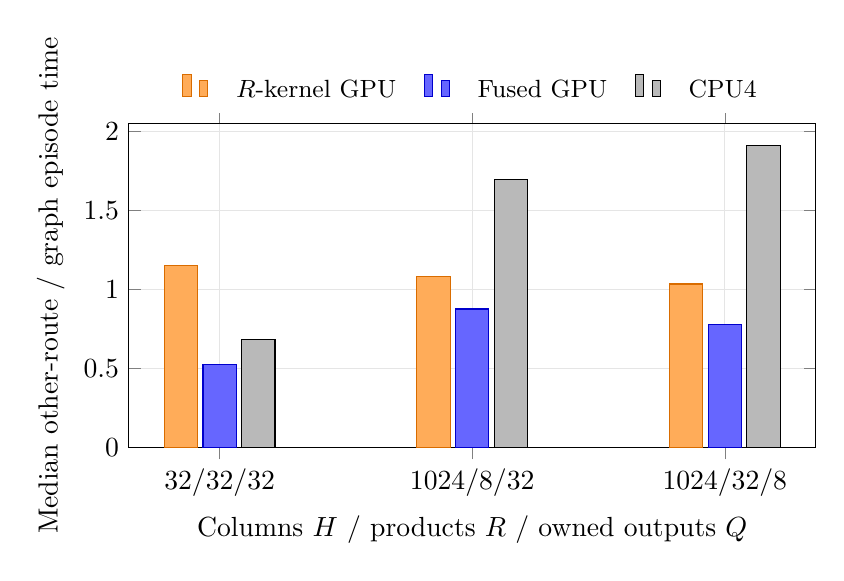
\begin{tikzpicture}
\begin{axis}[
 width=.85\linewidth,height=5.7cm,
 ybar,bar width=12pt,enlarge x limits=.18,
 ymin=0,ymax=2.05,ytick={0,.5,1,1.5,2},
 xtick={1,2,3},xticklabels={32/32/32,1024/8/32,1024/32/8},
 xlabel={Columns $H$ / products $R$ / owned outputs $Q$},
 ylabel={Median other-route / graph episode time},
 grid=major,grid style={gray!20},
 legend style={at={(.5,1.03)},anchor=south,legend columns=3,column sep=8pt,draw=none,fill=white,font=\small},
]
\addplot+[fill=orange!65,draw=orange!85!black,mark=none] coordinates {(1,1.150) (2,1.083) (3,1.034)};
\addplot+[fill=blue!60,draw=blue!80!black,mark=none] coordinates {(1,.525) (2,.876) (3,.779)};
\addplot+[fill=gray!55,draw=black,mark=none] coordinates {(1,.682) (2,1.694) (3,1.912)};
\legend{$R$-kernel GPU,Fused GPU,CPU4}
\end{axis}
\end{tikzpicture}}
\caption{Paired complete-episode median ratios over 16 dimension/family/order pairs per workload; above one favors the graph. It wins 15/16, 16/16, and 15/16 pairs over ordinary $R$-kernel GPU, but 0/16 over fusion at every workload. At the narrow $(32,32,32)$ workload it also wins 0/16 over CPU4. Capture, instantiation, and all $Q$ final host outputs are included~\cite{residentgraph}.}
\label{fig:resident-graph}
\end{figure}
\FloatBarrier

The graph's median ordinary-GPU/graph ratios are 1.150, 1.083, and 1.034: capturing repeated submissions can help compared with launching $R$ kernels afresh. Its fused-GPU/graph ratios are 0.525, 0.876, and 0.779, with \emph{zero} wins against fusion in all three sets of 16 complete episodes. Warm comparisons also favor fusion in 0/16 graph wins per workload; graph build is costlier than ordinary resident-GPU build. At $(32,32,32)$ the graph loses all 16 complete episodes to CPU4 (median CPU4/graph ratio 0.682). At the two wider workloads it wins 16/16 against CPU4, with median ratios 1.694 and 1.912. These ratios are medians of within-pair median ratios, not pooled times or confidence intervals. The graph's initial capture and instantiation are amortized over $Q$ \emph{identical-value} sums, a favorable case that does not establish performance when coefficients change~\cite{residentgraph}.

The same qualified campaign also pairs \emph{fusion} with CPU4 at $(H,R,Q)=(32,32,32)$: fusion wins 16/16 complete episodes, with median CPU4/fused ratio 1.342. In 8D low-rank support and the first order, the 32 owned sums take 2.581~ms on CPU4 versus 2.082~ms with fusion. The earlier \emph{single-output} $H=32,R=32$ fusion screen won only 22/72 episodes against CPU4, but it was a separate campaign with a different grid. This contrast is not a paired estimate of the effect of $Q$; it makes session length an explicit variable for future route-selection experiments~\cite{residentfusion,residentgraph}.

The first attempt qualified only 188/192 cases: a 0.2~s measurement window expired before four long CPU4 cases at $(1\,024,8,32)$ produced seven samples. Its archive remains excluded. The second campaign raised the episode window to 10~s, qualified all 192 cases, and alone supplies the plotted ratios. Peak process RSS was 2.17~GB, while peak VRAM was not measured. The display GPU showed 23\% use before the qualified run and 54\% after; the operator's no-other-user-computation label is not certified hardware isolation. For these three workloads the graph is a secondary research option behind fusion, not an automatic route. CPU1 is absent from this paired graph pilot, and no C++ implementation has a matched contract. Input updates, VRAM pressure, more dimensions, and downstream uses that keep intermediate outputs on GPU require separate experiments~\cite{residentgraph}.

\paragraph{What does an instrumented GPU trace explain?}
Source-unchanged CUPTI traces of the three oracle-checked resident GPU routes show what each launches (Figure~\ref{fig:resident-cupti-counts}). At $R=32$, ordinary GPU submits 33 operations and executes 32 accumulation kernels, CUDA Graph submits once but executes 32, and fusion submits and executes one. Initial packing and graph capture are excluded~\cite{residentcupti}.

\begin{figure}[!htbp]
\centering
\IfFileExists{exploratory_resident-cupti-counts.pdf}{\includegraphics[width=.92\linewidth]{exploratory_resident-cupti-counts.pdf}}{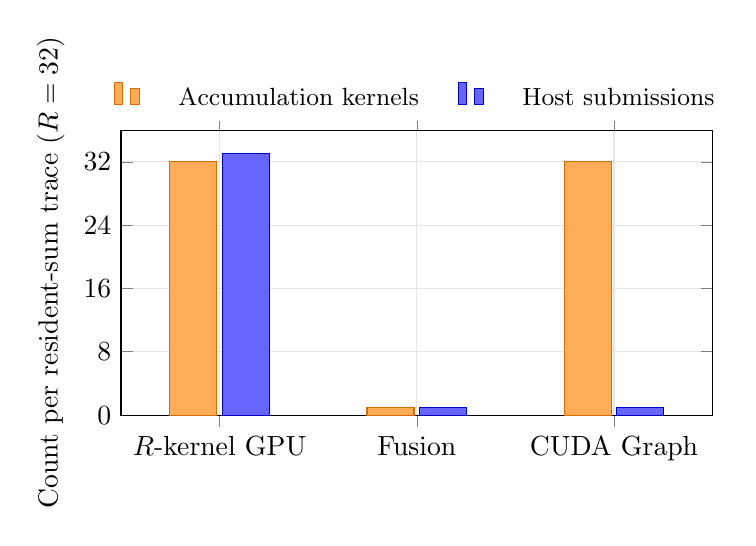
\begin{tikzpicture}
\begin{axis}[
 width=.75\linewidth,height=5.2cm,
 ybar,bar width=17pt,enlarge x limits=.25,
 ymin=0,ymax=36,ytick={0,8,16,24,32},
 xtick={1,2,3},xticklabels={$R$-kernel GPU,Fusion,CUDA Graph},
 ylabel={Count per resident-sum trace ($R=32$)},
 grid=major,grid style={gray!20},
 legend style={at={(.5,1.03)},anchor=south,legend columns=2,column sep=12pt,draw=none,fill=white,font=\small},
]
\addplot+[fill=orange!65,draw=orange!85!black,mark=none] coordinates {(1,32) (2,1) (3,32)};
\addplot+[fill=blue!60,draw=blue!80!black,mark=none] coordinates {(1,33) (2,1) (3,1)};
\legend{Accumulation kernels,Host submissions}
\end{axis}
\end{tikzpicture}}
\caption{CUPTI event counts with the same exact resident sum and one final host output. Ordinary GPU's 33rd submission resets the partial sum; one graph launch submits its captured reset and 32 kernels. These counts describe execution structure, not a speed ranking~\cite{residentcupti}.}
\label{fig:resident-cupti-counts}
\end{figure}
\FloatBarrier

The twelve traces cover 8D/65D, $H=32,1\,024$, $R=32$, \code{higher\_rank} support, and a positive metric. Every route passes the independent exact oracle before and after tracing and copies one final owned matrix to the host. In 8D at $H=32$, instrumented GPU-busy time is 157.83, 71.05, and 149.97~\(\mu\)s for ordinary GPU, fusion, and graph. In 65D at $H=1\,024$, it is 1.55, 1.17, and 1.53~ms; the corresponding final device-to-host copies take about 174, 159, and 175~\(\mu\)s. These traces diagnose repeated kernel and sum-buffer activity, but CUPTI changes durations, each trace is a single instrumented observation, and preparation is excluded. \emph{Only the uninstrumented paired PerfChecker campaigns above rank complete-episode speed.} Free VRAM was sampled only before and after, not at its peak; the display GPU showed 22\% use before tracing and 3\% after. No cause for every timing ratio or automatic routing rule follows from these traces~\cite{residentcupti}.

\Needspace{9\baselineskip}
\paragraph{What happens when no CUDA device is visible?}
An earlier \emph{functional} resident-sum test runs Julia 1.13 with four threads and \code{CUDA\_VISIBLE\_DEVICES=-1}, for which \code{CUDA.functional()} is false. It passes 3\,906\,890/3\,906\,890 assertions under forced bounds checks and again under automatic checks. Across 8D/65D, two support families, positive/mixed/degenerate signatures, $H=1,32,1\,024$, and $R=1,16$, sequential and four-thread CPU sums agree with the independent integer oracle and return distinct outputs; construction of the GPU route rejects cleanly. This establishes a CPU functional fallback when the device is \emph{masked}. It is not a speed measurement or a test on a machine physically lacking a GPU~\cite{residentcpuonly}.

\subsection{High ambient dimensions with fixed active support}
\label{sec:resident-highdim}
\paragraph{Why test this workload?}
The preceding resident-sum screens stop at 128D. Above that boundary, blade masks use \code{BigInt}; whether the resident routes remain feasible also depends on metric representation, preparation, and memory. This screen raises the ambient dimension from 129 to 8\,192 while fixing the \code{higher\_rank} fixture at twelve active directions, 576 product paths, and 224 output coefficients per column. It therefore probes ambient-size overhead and mask width for a \emph{fixed sparse task}; it does not test a support that grows with $n$ or a full middle grade. The positive metric remains a \code{Diagonal} inside \code{GeometricAlgebra}, as checked by its type and \code{Base.summarysize}: it occupies 1\,080 bytes at 129D, 32\,816 at 4\,096D, and 65\,584 at 8\,192D. An initial proposed 8\,192D refusal incorrectly assumed a dense metric matrix and was withdrawn. This screen sets no intrinsic 4\,096D or 8\,192D limit~\cite{residenthighdim}.

\paragraph{What is compared and validated?}
Four pairs of packed operands are prepared once. Each route accumulates \emph{all} contributions from $R$ products into a sum, then returns $Q$ distinct, independently owned host matrices. The matched routes are four-thread CPU (CPU4), ordinary GPU with $R$ accumulation kernels, one-kernel fused GPU, and a captured CUDA Graph. They share coefficients, paths, and addition order per output coefficient. An independent \code{Int64} oracle formed by insertion in basis words verifies every route before and after sampling. GPU functional tests pass 215\,103/215\,103 assertions with forced bounds checks and again with automatic checks across the ten high dimensions at $H=32,R=8$ and a positive metric. With CUDA masked, a later rerun of the 8D/65D CPU corpus passes 3\,906\,891 assertions and the high-dimensional extension 143\,401, \emph{per bounds policy}; GPU construction rejects cleanly. This functional fallback does not reproduce a machine physically lacking a GPU~\cite{residenthighdim}.

\paragraph{How are complete episodes measured?}
The ten dimensions are 129, 192, 256, 384, 512, 768, 1\,024, 2\,048, 4\,096, and 8\,192. Julia 1.13.0, CUDA.jl 6.4.0, and PerfChecker 1.0.0-rc1 run with four Julia threads, one BLAS thread, \code{-O2}, native CPU target, IEEE math, and automatic bounds checks on an RTX 3060 Ti with 8~GiB. A fresh process per dimension releases the previous resident data. The two workloads are $(H,R,Q)=(32,32,32)$ and $(1\,024,32,8)$. Four balanced route orders give 32 cases per dimension; seven samples each of build, hot, and complete episode give 672 observations per dimension, or 320/320 qualified cases and 6\,720 observations overall. Build includes resident preparation and graph capture where applicable; hot returns one fresh owned sum; the \emph{directly timed} episode constructs residents and returns all $Q$ owned sums. First calls, including JIT work, are archived separately. The performance grid uses a positive metric and repeated input values, not changing coefficients between the $Q$ sums~\cite{residenthighdim}.

\begin{table}[!htbp]
\centering\small
\begin{tabular}{@{}rccc@{}}
\toprule
Ambient $n$ & $32/32/32$ & $1\,024/32/8$ & Peak RSS (GiB) \\
\midrule
129 & 1.451 & 2.328 & 2.16 \\
192 & 1.469 & 2.482 & 2.23 \\
256 & 1.445 & 1.912 & 2.37 \\
384 & 1.464 & 2.170 & 2.79 \\
512 & 1.448 & 2.260 & 2.99 \\
768 & 1.474 & 2.190 & 3.01 \\
1\,024 & 1.472 & 2.077 & 2.98 \\
2\,048 & 1.513 & 1.883 & 3.94 \\
4\,096 & 1.426 & 1.582 & 4.04 \\
8\,192 & 1.280 & 1.377 & 5.58 \\
\bottomrule
\end{tabular}
\caption{Median of four paired CPU4/fused-GPU \emph{complete-episode} ratios at each dimension and workload $H/R/Q$; above one favors fusion. Each case first contributes the median of seven samples. Peak RSS is from its separate Julia process, under a 6~GiB budget; it is not peak VRAM. These ten rows are the qualified archives only~\cite{residenthighdim}.}
\label{tab:resident-highdim}
\end{table}

\FloatBarrier

\paragraph{What do the differences mean?}
Across the 40 order-specific pairs per workload, fusion beats CPU4 in 40/40, with median CPU4/fusion ratios 1.451 and 2.126 for the narrow and wide workloads. It also beats the ordinary $R$-kernel GPU in 40/40 per workload (median ordinary/fusion 1.765 and 1.216) and the graph in 40/40 (median fusion/graph 0.648 and 0.858). These are medians of \emph{paired case ratios}, not ratios of pooled times or uncertainty intervals. At 129D versus 8\,192D for $(1\,024,32,8)$, the fused build phase grows from 2.79 to about 34.5~ms while its one-output hot phase stays near 1.31--1.40~ms. Complete-episode medians move from 30.91/13.29~ms (CPU4/fusion) to 63.12/45.84~ms. Preparation is therefore a plausible contributor to the narrower advantage at 8\,192D; the follow-up profile in Section~\ref{sec:packonce} identifies repeated metric and basis validation within the batch~\cite{residenthighdim,packonce}.

\begin{figure}[!htbp]
\centering
\IfFileExists{exploratory_resident-highdim.pdf}{\includegraphics[width=.92\linewidth]{exploratory_resident-highdim.pdf}}{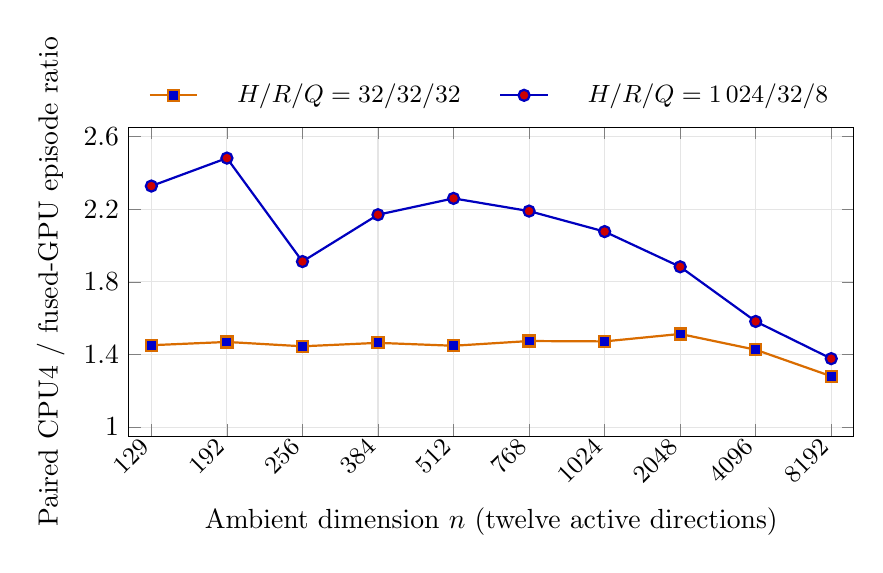
\begin{tikzpicture}
\begin{axis}[
 width=.89\linewidth,height=5.5cm,
 xmin=.7,xmax=10.3,ymin=.95,ymax=2.65,
 xtick={1,2,3,4,5,6,7,8,9,10},
 xticklabels={129,192,256,384,512,768,1024,2048,4096,8192},
 x tick label style={rotate=45,anchor=east,font=\small},
 xlabel={Ambient dimension $n$ (twelve active directions)},
 ylabel={Paired CPU4 / fused-GPU episode ratio},
 ytick={1,1.4,1.8,2.2,2.6},
 grid=major,grid style={gray!20},
 legend style={at={(.5,1.03)},anchor=south,legend columns=2,column sep=12pt,draw=none,fill=white,font=\small},
]
\addplot+[orange!85!black,thick,mark=square*,mark size=2pt] coordinates {(1,1.451) (2,1.469) (3,1.445) (4,1.464) (5,1.448) (6,1.474) (7,1.472) (8,1.513) (9,1.426) (10,1.280)};
\addplot+[blue!75!black,thick,mark=*,mark size=2pt] coordinates {(1,2.328) (2,2.482) (3,1.912) (4,2.170) (5,2.260) (6,2.190) (7,2.077) (8,1.883) (9,1.582) (10,1.377)};
\legend{$H/R/Q=32/32/32$,$H/R/Q=1\,024/32/8$}
\end{axis}
\end{tikzpicture}}
\caption{The same paired ratios as Table~\ref{tab:resident-highdim}. Fusion wins at every point; its margin for the wider workload narrows toward the largest tested dimensions. The fixed support and separately measured preparation rule out interpreting this curve as scaling for dense high-dimensional products~\cite{residenthighdim}.}
\label{fig:resident-highdim}
\end{figure}
\FloatBarrier

\paragraph{Provenance, limits, and next test.}
The nine retained manifests through 4\,096D share prefix \code{garamonbench-resident-highdim-} and suffix \code{n<D>-isolated-unified-20260928/}, with $D=129,192,256,384,512,768,1024,2048,4096$. The 8\,192D archive has the same prefix and suffix \code{n8192-isolated-v3-20260928/}. Their manifests share source fingerprint \code{10445c4990573c83}\allowbreak\code{e81416f0edb93a46}\allowbreak\code{59de235c7bd84f1a}\allowbreak\code{e0242e28d545fc84}. Earlier interrupted or invalid attempts are excluded: a multi-dimension process exhausted its 4~GiB RSS budget at 768D, an initial 4\,096D run failed before measurement, and initial 8\,192D attempts lacked samples or failed before measurement. The retained ten fresh-process runs use a 6~GiB RSS cap; 8\,192D peaks at 5.58~GiB, which is an operational observation rather than a dimensional limit. Peak VRAM was not measured. The \code{isolated} label records no other declared user computation, while the display GPU remained active. The next subsection reports the completed build profile and its exact optimization. Remaining tests should vary active directions, grades, signatures, and values between outputs, measure peak VRAM and a GPU-resident consumer, and compare 1/2/4/8/16 CPU threads under stricter isolation. A matched C++ comparison requires a route with the same arithmetic and outputs. No automatic selector or general high-dimensional speed claim follows~\cite{residenthighdim}.

\subsection{Validating the algebra once per homogeneous packed batch}
\label{sec:packonce}
\paragraph{Why optimize preparation?}
The initial fixed-support screen found a rising fused-GPU build cost with ambient dimension, although its one-output hot call changed little. A PerfChecker CPU profile of the 8\,192D, $H=1\,024$ resident build located repeated work in \code{src/plans.jl:74--83}: for every packed column, the old path rescanned the diagonal metric and compared basis names, even when all columns reused the \emph{same algebra object} as the plan. This is validation overhead, not additional Clifford products. The revised \code{pack\_product\_batch} checks object identity across the batch, validates the metric and basis snapshot on entry and exit, then packs the columns. If algebra objects differ, it retains the original per-column validation. Tests still reject a metric or basis mutation before a call and cover distinct but equivalent algebras. No coefficient or product path is omitted. The contract excludes concurrent mutation during packing; entry/exit checks detect a persistent change, not a transient change that is restored before exit~\cite{packonce}.

\paragraph{How were the two versions checked?}
The before and after versions each have ten fresh-process archives over the same dimensions, hardware, fixed twelve-direction support, positive diagonal metric, four routes, four balanced orders, and $(H,R,Q)=(32,32,32)$ or $(1\,024,32,8)$. Each campaign independently qualifies 320/320 cases and 6\,720 observations, with seven samples per build, hot, and complete-episode phase. The old fingerprint is recorded in Section~\ref{sec:resident-highdim}; the optimized manifests share \code{94f805ca8d638c18}\allowbreak\code{770001ed75f40e8b}\allowbreak\code{f81f3767fdc240ec}\allowbreak\code{a5f32798c9fa1a77}. The archives are separate runs rather than temporally paired before/after samples. Within \emph{each} version, route comparisons remain paired by fixture and order. Every measured case passes the independent integer oracle before and after sampling. After the change, the main Garamon suite passes 6\,034/6\,034 assertions with forced bounds checks and again with automatic checks; the high-dimensional GPU suite passes 215\,103/215\,103 per policy, and the CPU route with CUDA masked passes 3\,906\,891 plus 143\,401 per policy. The direct complete episode, rather than a sum of build and hot medians, determines the speed result~\cite{packonce}.

\begin{table}[!htbp]
\centering\small
\begin{tabular}{@{}rcccc@{}}
\toprule
$n$ & Fused build, old $\to$ new (ms) & Gain & Fused episode, old $\to$ new (ms) & Gain \\
\midrule
129 & 2.79 $\to$ 2.15 & 1.30 & 13.29 $\to$ 14.15 & 0.94 \\
192 & 3.02 $\to$ 2.10 & 1.44 & 12.95 $\to$ 12.95 & 1.00 \\
256 & 3.33 $\to$ 2.12 & 1.57 & 16.60 $\to$ 14.88 & 1.12 \\
384 & 3.77 $\to$ 2.11 & 1.79 & 14.73 $\to$ 12.02 & 1.23 \\
512 & 4.43 $\to$ 2.15 & 2.06 & 14.39 $\to$ 12.65 & 1.14 \\
768 & 5.34 $\to$ 2.14 & 2.49 & 15.45 $\to$ 12.19 & 1.27 \\
1\,024 & 6.43 $\to$ 2.19 & 2.93 & 16.78 $\to$ 11.93 & 1.41 \\
2\,048 & 10.37 $\to$ 2.15 & 4.81 & 20.67 $\to$ 12.55 & 1.65 \\
4\,096 & 18.56 $\to$ 2.26 & 8.21 & 29.63 $\to$ 13.03 & 2.27 \\
8\,192 & 34.43 $\to$ 2.28 & 15.11 & 45.84 $\to$ 12.50 & 3.67 \\
\bottomrule
\end{tabular}
\caption{Fused GPU preparation and complete-episode medians for $(H,R,Q)=(1\,024,32,8)$. Each displayed time is the median across four route-order cases, after the seven samples in each case are summarized. Gain is old/new; above one favors grouped validation. These are distinct before and after campaigns, not sample-level pairs~\cite{packonce}.}
\label{tab:packonce}
\end{table}
\FloatBarrier

\paragraph{What did the optimization change?}
Build time improves in 10/10 dimensions, with median old/new factor 2.28; the complete episode improves in 9/10, median 1.25. At 8\,192D, build falls from 34.43 to 2.28~ms (15.11-fold) and the episode from 45.84 to 12.50~ms (3.67-fold). At 129D the episode instead rises from 13.29 to 14.15~ms despite a faster build, while 192D is essentially unchanged. In the narrower $(32,32,32)$ workload, build improves in 10/10 dimensions (median factor 1.09), but episodes improve in only 7/10 (median factor 1.03). Thus reducing validation cost need not improve a complete session when other phases dominate. At 8\,192D in the wide workload, median fused-episode CPU allocation remains 19.10~MiB before and after; the measured gain chiefly removes repeated scanning rather than allocated bytes. PerfChecker records zero GC time in the sampled phases of both campaigns, without characterizing first calls or later memory pressure~\cite{packonce}.

\begin{figure}[!htbp]
\centering
\IfFileExists{exploratory_packonce.pdf}{\includegraphics[width=.92\linewidth]{exploratory_packonce.pdf}}{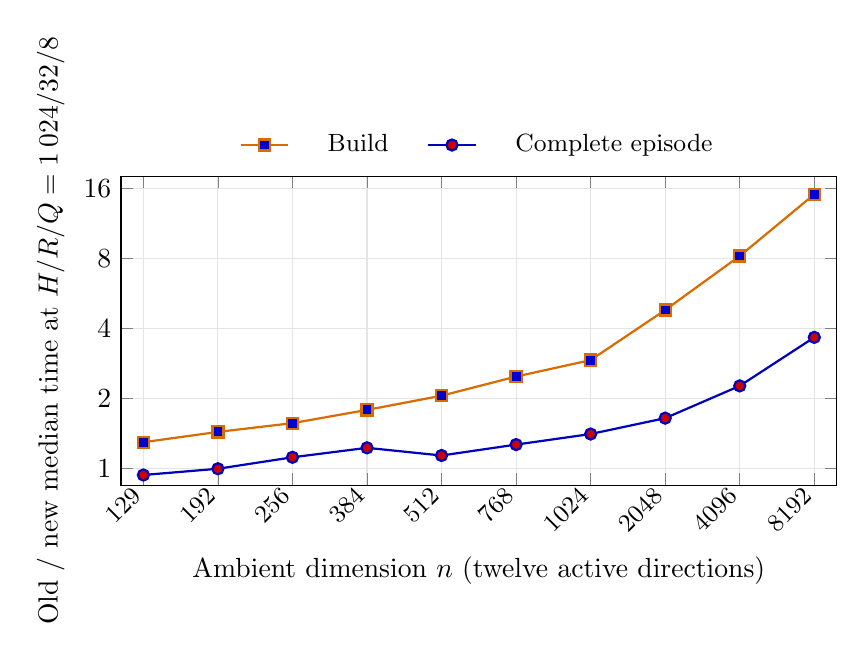
\begin{tikzpicture}
\begin{axis}[
 width=.88\linewidth,height=5.5cm,
 ymode=log,log basis y=2,ymin=.85,ymax=18,
 ytick={1,2,4,8,16},yticklabels={1,2,4,8,16},
 xmin=.7,xmax=10.3,xtick={1,2,3,4,5,6,7,8,9,10},
 xticklabels={129,192,256,384,512,768,1024,2048,4096,8192},
 x tick label style={rotate=45,anchor=east,font=\small},
 xlabel={Ambient dimension $n$ (twelve active directions)},
 ylabel={Old / new median time at $H/R/Q=1\,024/32/8$},
 grid=major,grid style={gray!20},
 legend style={at={(.5,1.03)},anchor=south,legend columns=2,column sep=12pt,draw=none,fill=white,font=\small},
]
\addplot+[orange!85!black,thick,mark=square*,mark size=2pt] coordinates {(1,1.30) (2,1.44) (3,1.57) (4,1.79) (5,2.06) (6,2.49) (7,2.93) (8,4.81) (9,8.21) (10,15.11)};
\addplot+[blue!75!black,thick,mark=*,mark size=2pt] coordinates {(1,.94) (2,1.00) (3,1.12) (4,1.23) (5,1.14) (6,1.27) (7,1.41) (8,1.65) (9,2.27) (10,3.67)};
\legend{Build,Complete episode}
\end{axis}
\end{tikzpicture}}
\caption{Before/after gain factors from Table~\ref{tab:packonce}. The logarithmic vertical axis shows how removing repeated algebra validation affects preparation more strongly than the full session. Values at or below one do not improve the measured episode~\cite{packonce}.}
\label{fig:packonce}
\end{figure}
\FloatBarrier

\paragraph{Do the four routes keep the same ranking?}
Within the optimized campaign, fusion beats CPU4 in 40/40 paired complete episodes at each workload, with median CPU4/fusion ratios 1.459 and 2.429. It beats the ordinary $R$-kernel GPU in 40/40 at $(32,32,32)$ and 38/40 at $(1\,024,32,8)$, with median ordinary/fusion ratios 1.818 and 1.310. The graph loses to fusion in 40/40 at each workload; median fusion/graph ratios are 0.637 and 0.817. These \emph{within-campaign} comparisons are paired. The old/new factors in Table~\ref{tab:packonce} compare separate fresh-process campaigns under the same nominal setup; they are descriptive improvements, not a pooled causal estimate. The unchanged arithmetic and oracle plus the profile support the repeated-validation explanation for build time, while display-GPU activity and uncontrolled hardware isolation limit broader ranking claims~\cite{packonce}.

\paragraph{What does profiling leave to do?}
Before modification, an exploratory CPU profile attributed 315 samples to diagonal traversal at \code{src/plans.jl:83}; it has no comparable folded-stack archive. The ten optimized manifests use the \code{garamonbench-resident-highdim-} prefix and \code{n<D>-isolated-packonce-20260928/} suffix. Two reproducible optimized profiles at 129D and 8\,192D/$H=1\,024$ now retain folded stacks and CPU/allocation SVG flame graphs. The 8\,192D profile records 1\,187 CPU samples: only 17, 5, and 5 are attributed to the old validation sites at lines 74, 79, and 83, while packed-matrix allocation at line 236 has 224 and column copies at lines 247--259 remain visible. These are line-attributed samples, not exclusive percentages or uninstrumented speed measurements. The next comparison should isolate copying and packed-matrix allocation, including a possible exact cyclic four-column representation, while retaining changed-value, signature, support, host-output, VRAM, and mutation contracts. The upstream C++ generator has no matched resident route; no automatic GPU threshold or language winner follows~\cite{packonce}.

\section{Structural techniques: why test them?}
\label{sec:transpositions}
Each of the following fifteen mechanisms addresses a specific workload. For measured prototypes, the principle is followed immediately by the protocol, figure, and interpretation. For proposed mechanisms, the experiment is an \emph{open question}; no Garamon speed result is assigned to it. Table~\ref{tab:questionsstructurelles} separates three easily confused sources of savings: fewer masks, cheaper coefficient arithmetic, and fewer instructions. It also locates four measured prototypes without ranking them against one another.

\begin{table}[ht]
\centering\small
\begin{tabularx}{\linewidth}{@{}p{40mm}X X@{}}
\toprule
Technique and status & Why test it? & Relevant comparison \\
\midrule
N01: binary ranking & Ambient dimension is large, but the observed masks span few independent directions. & Total cost of compact support representation versus sparse traversal and a prepared plan, across reuse horizons. \\
N03: radical & A degenerate metric may reduce inversion to a smaller quotient. & Quotient inversion plus a finite series versus complete regular-matrix inversion. \\
N04: short identity & The same input satisfies $A^2=\lambda1$ and is raised to many powers. & Certify once and reuse versus direct or binary powering, including fallback. \\
N05: Pfaffian & Only the scalar coefficient of a vector chain is requested. & Contractions and a Pfaffian versus admissible baselines with the same scalar output. \\
Verified superoptimization: proposed & The same paths repeatedly execute short sign and indexing loops. & Proven equivalent instructions within one fixed kernel, then total time and code size. \\
Exact multimodular arithmetic: proposed & Large exact coefficients make the oracle or integer product expensive. & Modular computation and reconstruction versus direct \code{BigInt} or rational arithmetic, including the exactness proof. \\
\bottomrule
\end{tabularx}
\caption{The workload motivating each technique and the comparison that would establish its value. The first four have Garamon trials below; the last two have no Garamon performance measurement.}
\label{tab:questionsstructurelles}
\end{table}

The binary-ranking, nilpotent-radical, and Pfaffian prototypes have exploratory measurements under \code{perf/}, discussed in Sections~\ref{sec:n01perf}, \ref{sec:n03perf}, and~\ref{sec:n05perf}. N04 also has correctness tests and an initial exploratory timing smoke test~\cite{n04smoke}. The remaining eleven mechanisms have neither an implementation nor Garamon timing data. Their references establish results in their original domains, not transferred Garamon speedups. Every future comparison must preserve its requested output contract: full multivector, projection, scalar, or decision. Potential algebraic savings must be weighed against detection, conversion, preparation, and memory costs.

\paragraph{Common measurement conditions.}
Measurements come from reports and CSV files supplied with this manuscript and from two documented \code{perf/} campaigns in the Julia repository. They use Julia 1.13.0 and an Intel Core i7-12700. Most use PerfChecker; generation and precompilation have separate harnesses. Repetition counts and uncertainty estimates differ across families, so times from different campaigns do not form one paired benchmark. Étendue3D computations shared the machine during several earlier campaigns. The later B1W replay, matched Julia/C++ replays, packed GPU and four-thread CPU pilots, resident-sum and fusion screens, focused replay, and CUDA Graph pilot had no other declared user computation, but that status does not establish hardware isolation. The CUPTI profiles are diagnostics, not uninstrumented timing samples. Timing rankings remain \emph{exploratory}; validated case counts establish correctness only for their tested fixtures.

For the dimension, workspace, precompilation, and long-trace campaigns, independent small-integer oracles count basis-index inversions. The \code{Float64} sums in those fixtures are exactly representable within stated bounds. Generated products are compared with Garamon.jl's direct product. The approximate-pruning experiment uses a rational oracle and records floating-point error separately. These checks do not establish exact floating-point behavior for every product.

\subsection{Binary ranking of supports}
\paragraph{Why consider it?}
A high ambient dimension does not mean that a product uses every basis direction. The binary rank $d$ is the number of independent masks needed to generate the encountered masks under XOR. Two independent masks, for example, generate only four masks even in an algebra with 128 directions. N01 targets expressions with restricted support: in principle, addressing and storage can range over $2^d$ masks rather than $2^n$. The experiment must determine whether this saving repays plan construction, validation, and the outputs actually requested.

Pauli strings also use binary vectors, XOR, and bit operations~\cite{paulib}. In an \emph{orthogonal} basis, Equation~\eqref{eq:blade} likewise gives output mask $A\oplus B$. If the masks in an expression span a rank-$d$ subspace over $\mathbb F_2$, its products can reach at most $2^d$ masks, versus $2^n$ in the ambient algebra. Permutation signs and metric factors still have to be computed: this closure is not an automatic identification with $\Cl(d,0)$.

The first N01 prototype compares two-factor products with fixed supports and a complete output. The more ambitious target is a long expression whose supports change but remain in a small binary subspace. That would require a basis certificate propagated only through operations known to preserve the subspace. A negative case should increase rank at every step. Nonorthogonal metrics need a separate closure proof.

\paragraph{N01 experiment: observed complete episodes.}
\label{sec:n01perf}
The measured question is how many products must reuse the same supports before N01 costs less than a prepared plan or the current sparse traversal. Figure~\ref{fig:n01horizon} compares \emph{complete episodes}, including construction and retained owned outputs. The $2^d$ bound motivates the experiment but does not predict time. N01 remains a prototype under \code{perf/}, outside the public core and selector~\cite{n01report}. It compresses support addressing in an orthogonal basis while retaining ambient masks, grades, signs, and metric factors; it still traverses input pairs. All 676 correctness and contract assertions pass.

A one-thread PerfChecker campaign validates 648/648 cases. Two passes reverse route order across 12 dimensions from 4 to 128, three support families, three reuse horizons, and three routes: current sparse traversal, prepared plan, and N01. Positive, indefinite, and degenerate diagonal metrics rotate with dimension; this is not an exhaustive dimension-by-signature cross. An independent \code{Int64} oracle checks every coefficient for small integers exactly representable in \code{Float64}. Each timed episode constructs a fresh artifact, runs $H$ products, and retains all $H$ owned outputs. Median observed episode time divided by $H$ yields total time per product; it is not the sum of separate build and execution medians. The archive has 9\,396 raw samples: 1\,512 builds, 3\,942 warm executions, and 3\,942 complete episodes. An earlier additive 324-case screen is separate and not an end-to-end measurement. First compilation is recorded separately, rather than through a fresh process here.

\begin{figure}[ht]
\centering
\IfFileExists{exploratory_n01horizon.pdf}{\includegraphics[width=.92\linewidth]{exploratory_n01horizon.pdf}}{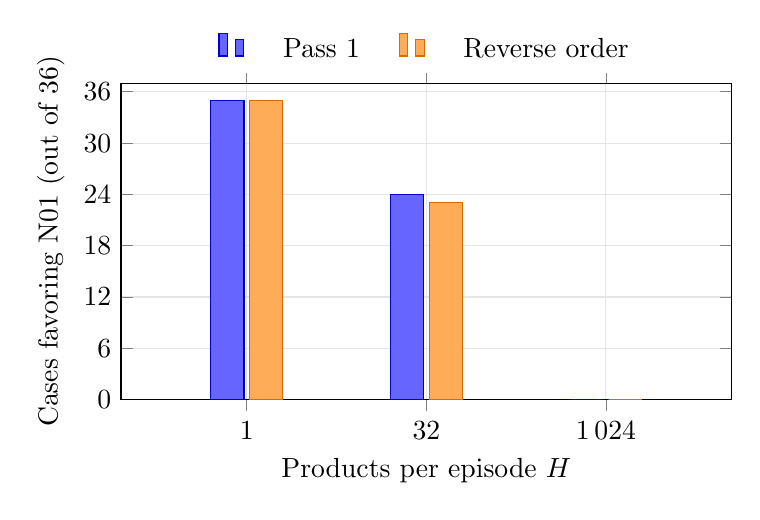
\begin{tikzpicture}
\begin{axis}[
 width=.77\linewidth,height=5.6cm,
 ybar,bar width=12pt,enlarge x limits=.35,
 ymin=0,ymax=37,ytick={0,6,12,18,24,30,36},
 xtick={1,2,3},xticklabels={1,32,1\,024},
 xlabel={Products per episode \(H\)},
 ylabel={Cases favoring N01 (out of 36)},
 grid=major,grid style={gray!20},
 legend style={at={(.5,1.03)},anchor=south,legend columns=2,column sep=12pt,draw=none,fill=white},
]
\addplot+[fill=blue!60,draw=blue!80!black,mark=none] coordinates
 {(1,35) (2,24) (3,0)};
\addplot+[fill=orange!65,draw=orange!85!black,mark=none] coordinates
 {(1,35) (2,23) (3,0)};
\legend{Pass 1,Reverse order}
\end{axis}
\end{tikzpicture}}
\caption{N01 versus the \emph{same prepared plan} on directly observed complete-episode cost, including construction and retained outputs. At $H=32$, N01 wins 23 configurations in both passes. Zero bars at $H=1\,024$ mean 0/36 wins in each pass, not missing data. Exploratory timings~\cite{n01report}.}
\label{fig:n01horizon}
\end{figure}
\FloatBarrier

Against the prepared plan, N01 has a lower complete-episode median in 35/36 configurations at $H=1$ in each pass, 24/36 and 23/36 at $H=32$ (23 common wins), and 0/36 at $H=1\,024$. Against current sparse traversal, it wins 31/36 at $H=1$ and 36/36 at both longer horizons in each pass. The $2^d$ output table and pairwise factors may explain the loss to the prepared plan at high reuse or rank, but this causal account remains untested. Reversing route order does not remove Étendue3D interference; rankings need an isolated rerun with matched conditions. A broader 10\,287-case manifest covering every integer dimension from 2 to 128 is prepared but \emph{not run}.

\paragraph{First K1v2 rerun batch.}
A separate campaign compares the core's exact prepared plan, N01, a compact-rank plan, and its workspace variant with matched inputs and owned outputs~\cite{k1decision}. Its K1v2 manifest has 41\,148 cases across 127 dimensions from 2 to 128, three support families, three metrics, three horizons, three output requests, and four routes, partitioned into 127 disjoint 324-case batches. Only the first, \code{n002}, has run: 324/324 qualified cases in 168.08~s, 5\,292 raw samples, and 0.768~GiB peak RSS. The oracle checked outputs before and after measurement. The audit finds 324 started, measured, and qualified cases without duplication; 40\,824 cases in \code{n003}--\code{n128} remain unrun~\cite{k1audit}. The recorded condition is \code{exploratory\_interference} with the \code{Etendue3D} label. This batch verifies partitioning and replay, not a stable ranking or selection threshold. Its times are not compared with the earlier N01 campaign.

\paragraph{B4 pilot: bounds checks in the compact-rank kernel.}
\emph{Why test it?} The K1 compact plan stores an $A\times B$ output-index matrix and cocycle factors. A zero output index marks an inadmissible pair; every other index is within the $O$ output slots. B4 asks whether bounds checks inside a repeatedly executed accumulation loop add measurable cost after a private workspace and its plan have been validated. The checked and locally annotated routes use the \emph{same} plan, eligible pairs, $j,i$ traversal order, per-call input checks, and independently owned sparse outputs. Construction checks metric finiteness, mask bounds, matrix shapes, output indices, unique output masks, and buffer lengths. This experimental workspace is neither shared concurrently nor mutated structurally during reuse; its Julia vectors remain mutable, so initial validation is not a guarantee against later mutation~\cite{b4bounds}.

\emph{Correctness and compiled loop.} Under Julia 1.13.0, the targeted suite passes 874/874 assertions with \code{--check-bounds=yes} and again with \code{--check-bounds=auto}. It covers dimensions 2, 8, 65, and 128, two support families, positive, mixed, and degenerate metrics, three output requests, \code{Float64} and \code{Int64}, rejection cases, and output ownership. An independent integer oracle checks coefficients. For one 8D signature, LLVM IR contains a \code{throw\_boundserror} path in checked accumulation under \code{auto}, absent from the annotated loop; under \code{yes}, the path occurs in both. This confirms the \emph{local} compiler effect, not removal of every product validation or a speedup. The 8D PerfChecker smoke test qualifies 16/16 cases and 336 observations; its four $H=1\,024$ route-order pairs favor annotation, but the largest ratio (1.248) is sensitive to concurrent load~\cite{b4bounds}.

\emph{Paired 12D experiments.} Two separate PerfChecker campaigns each qualify 288/288 cases and 6\,048 observations over dimensions 2, 3, 4, 6, 8, 12, 16, 32, 64, 65, 96, and 128, two support families, horizons $H=1,32,1\,024$, and two route orders. Both use a positive diagonal metric, automatic bounds checks, \code{-O2}, native CPU, one thread, seven samples per build, warm, and directly timed complete-episode phase, and an independent oracle before and after measurement. The first ran alongside Étendue3D. The second recorded no other user Julia/Garamon computation in process snapshots before and after, but its \code{isolated} label does \emph{not} certify hardware isolation. Figure~\ref{fig:b4bounds} shows complete-episode wins. Each median ratio is checked time divided by annotated time for one dimension, family, and order; the reported summary is the median of 48 such ratios, not a ratio of pooled times or an uncertainty interval~\cite{b4bounds}.

\begin{figure}[ht]
\centering
\IfFileExists{exploratory_b4bounds.pdf}{\includegraphics[width=.92\linewidth]{exploratory_b4bounds.pdf}}{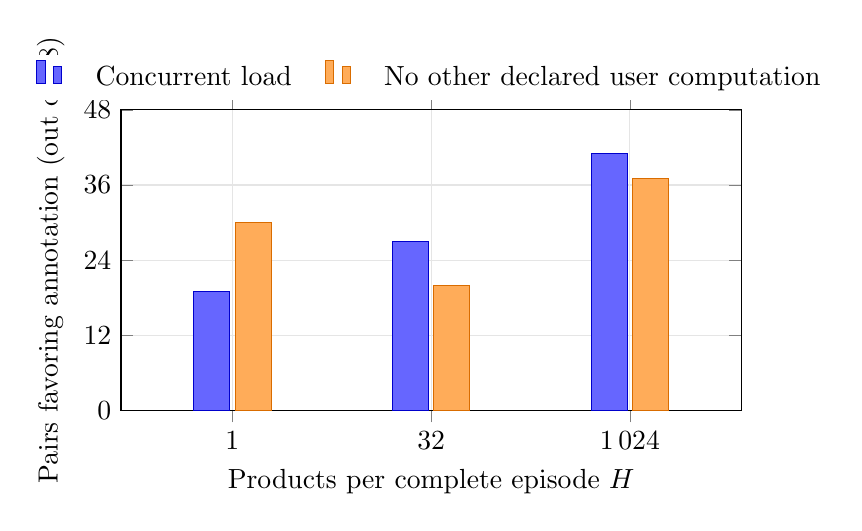
\begin{tikzpicture}
\begin{axis}[
 width=.78\linewidth,height=5.4cm,
 ybar,bar width=13pt,enlarge x limits=.28,
 ymin=0,ymax=48,ytick={0,12,24,36,48},
 xtick={1,2,3},xticklabels={1,32,1\,024},
 xlabel={Products per complete episode \(H\)},
 ylabel={Pairs favoring annotation (out of 48)},
 grid=major,grid style={gray!20},
 legend style={at={(.5,1.03)},anchor=south,legend columns=2,column sep=10pt,draw=none,fill=white},
]
\addplot+[fill=blue!60,draw=blue!80!black,mark=none] coordinates
 {(1,19) (2,27) (3,41)};
\addplot+[fill=orange!65,draw=orange!85!black,mark=none] coordinates
 {(1,30) (2,20) (3,37)};
\legend{Concurrent load,No other declared user computation}
\end{axis}
\end{tikzpicture}}
\caption{B4 complete-episode paired wins across 12 dimensions and two support families. Median checked/annotated ratios at $H=1,32,1\,024$ are respectively 0.993, 1.006, 1.032 under concurrent load and 1.018, 0.995, 1.031 in the separate run without other declared user computation. Both campaigns are exploratory; the second is not certified hardware isolation~\cite{b4bounds}.}
\label{fig:b4bounds}
\end{figure}
\FloatBarrier

At $H=1\,024$, annotation has the lower complete-episode median in 41/48 pairs under concurrent load, with a median paired ratio of 1.032, and in 37/48 pairs in the second campaign, with a median ratio of 1.031. At $H=32$ in the second campaign it wins 20/48, with a median ratio of 0.995. Warm-call allocation bytes are identical between routes in all 48 pairs at each horizon in both campaigns. One high-rank 12D cell in the second campaign showed a ratio near two, but two targeted reruns changed that result when the initial route order was reversed; it is a plausible order or warm-up artifact, \emph{not} a demonstrated twofold speedup. More controlled warm-up and frequency tracking are needed before a routing rule. The timed grids use supports generated by at most three or twelve directions (at most eight or 24 terms), not full central grades; mixed and degenerate metrics occur in correctness tests but not in these timing grids. No equivalent C++ kernel has been paired with B4~\cite{b4bounds}.

\FloatBarrier
\subsection{Invariant sectors}
\paragraph{Why consider it?}
The \emph{tapering} of the Hamiltonians of Pauli uses switching symmetries to restrict the calculation to a sector~\cite{bravyitaper}. For switching involutions $S_j$ , one can form $P_{\boldsymbol\epsilon}=\prod_j(1+\epsilon_j S_j)/2$ . A $P_{\boldsymbol\epsilon}AP_{\boldsymbol\epsilon}$ projection can then be calculated in a smaller block \emph{if} all the operators of the trace preserve this block. The possible gain is on the excluded sectors; a complete multi-vector output does not allow to erase them.

\paragraph{Proposed experiment; no Garamon measurements.}
The prototype will have to certify switching, involution, invariance and requested sector, then compare the projection obtained with that of a complete calculation. Terms that pair the sectors, or an output covering all sectors, serve as negative controls. The construction of the projectors and the conversion of the data are included in the total cost.

\subsection{Nilpotent filtration of degenerate metrics}
\paragraph{Why consider it?}
A degenerate metric has radical directions, whose nilpotence bounds the series needed to invert an element with an invertible quotient. N03 asks whether solving this smaller quotient first reduces the cost of a complete inverse after construction, finite-series products, and owned outputs are counted.

In a degenerate Clifford algebra, the radical $R$ of the quadratic form generates a nilpotent ideal~\cite{ablamowicz,bamberg}. If $\dim R=r$, the ideal $J$ of terms containing at least one radical direction satisfies $J^{r+1}=0$, and $\Cl(V)/J\simeq\Cl(W)$ for a nondegenerate complement $W$. Filtering by radical degree can therefore stop products beyond $r$ radical factors. For $A=q+j$ with $j\in J$, one must \emph{first} prove that the image $q$ is invertible in the quotient and compute $q^{-1}$. Only then does
\[
 A^{-1}=\sum_{k=0}^{r}(-q^{-1}j)^k q^{-1}
\]
provide a finite inverse. Factor order matters in this noncommutative algebra; a radical term cannot rescue a singular quotient.

The target is a \emph{genuinely} degenerate metric, including projective geometric algebra forms. A null vector in conformal geometric algebra does not by itself establish a radical, and a nondiagonal matrix with zero diagonal can be nondegenerate. N03 currently accepts an already diagonal metric, verifies the quotient inverse, and checks both $AA^{-1}=A^{-1}A=1$ with an independent rational oracle~\cite{n03report}. Basis changes, coefficient growth, and series products may erase the smaller quotient's saving. The experiment and its limitations follow.

\paragraph{N03 experiment: conditional inversion.}
\label{sec:n03perf}
The N03 prototype compares inversion by a left regular matrix over the full active subalgebra with inversion in the \emph{nondegenerate quotient}, followed by a finite radical series~\cite{n03report}. Both routes construct their inputs at each iteration and return the same sequence of independently owned inverse multivectors. An independent rational oracle checks every coefficient and both left and right inverse products. All 114 assertions pass, including expected rejection of singular quotients and treatment of isotropic vectors outside the radical. Another 72 checks cover the case grid, its partition, and a corrected signed-metric fixture with a nonradical direction.

The PerfChecker smoke test qualifies six of six route cases with 42 samples, seven per route. Dimensions 3, 4, and 5 have respectively one, two, and three radical axes, with two nonradical axes and horizon one. Metrics are already diagonal; general-metric decomposition is not timed. All measured inputs are invertible, have quotients dominated by a scalar part, and use \code{Float64} coefficients checked against the rational oracle under a declared tolerance. Medians and p95 times, in microseconds, are:

\begin{table}[ht]
\centering\small
\begin{tabular}{@{}crrrr@{}}
\toprule
$n/r$ & Regular med. & Radical med. & Regular p95 & Radical p95 \\
\midrule
$3/1$ & 19.252 & 15.830 & 44.025 & 43.590 \\
$4/2$ & 35.469 & 26.041 & 113.569 & 59.482 \\
$5/3$ & 60.028 & 39.888 & 193.544 & 73.751 \\
\bottomrule
\end{tabular}
\caption{First N03 smoke test: one thread, regular then radical order, with construction and output included. Seven samples per route under Étendue3D interference. The p95 values vary widely; no reproducible speed gain is established~\cite{n03report}.}
\label{tab:n03smoke}
\end{table}

The corrected extended screen spans twelve dimensions from 2 to 128, radical counts $r=1,2,3$, one or two active nonradical directions $s$, positive or signed quotients, three horizons, and both routes. Two fresh processes reverse route order; each qualifies 756/756 cases and retains 5\,292 raw samples, for 1\,512 cases and 10\,584 samples total~\cite{n03report,n03screen}. Their controller times are 154.49 and 155.73~s, with peak RSS of 728.62 and 715.46~MiB. The coverage audit finds no missing or duplicate qualified case. Maximum absolute deviation from the rational oracle is $5.55\times10^{-17}$. An earlier run with 396 successful cases and 360 generator errors for $s=1$ is archived separately and excluded after that branch was corrected and tested.

\begin{figure}[ht]
\centering
\IfFileExists{exploratory_n03screen.pdf}{\includegraphics[width=.92\linewidth]{exploratory_n03screen.pdf}}{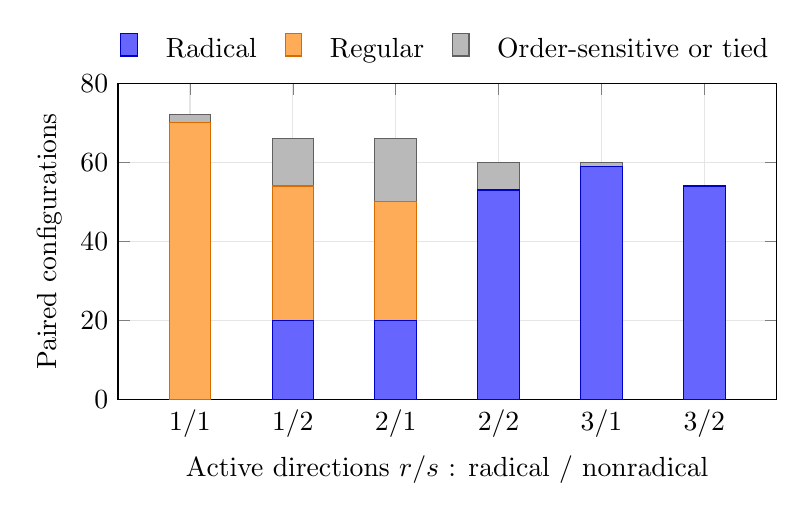
\begin{tikzpicture}
\begin{axis}[
 width=.82\linewidth,height=5.6cm,
 ybar stacked,bar width=15pt,enlarge x limits=.14,
 ymin=0,ymax=80,ytick={0,20,40,60,80},
 xtick={1,2,3,4,5,6},
 xticklabels={$1/1$,$1/2$,$2/1$,$2/2$,$3/1$,$3/2$},
 xlabel={Active directions \(r/s\) : radical / nonradical},
 ylabel={Paired configurations},
 grid=major,grid style={gray!20},
 legend style={at={(.5,1.03)},anchor=south,legend columns=3,column sep=8pt,draw=none,fill=white},
]
\addplot+[fill=blue!60,draw=blue!80!black,mark=none] coordinates
 {(1,0) (2,20) (3,20) (4,53) (5,59) (6,54)};
\addplot+[fill=orange!65,draw=orange!85!black,mark=none] coordinates
 {(1,70) (2,34) (3,30) (4,0) (5,0) (6,0)};
\addplot+[fill=gray!55,draw=gray!75!black,mark=none] coordinates
 {(1,2) (2,12) (3,16) (4,7) (5,1) (6,0)};
\legend{Radical,Regular,Order-sensitive or tied}
\end{axis}
\end{tikzpicture}}
\caption{N03 screen of 378 configurations paired across two orders. Color identifies the method with the lower complete-episode median in \emph{both} orders; the other 38 configurations switch choice or tie. One-thread exploratory comparison under Étendue3D load, with families and horizons grouped by $r/s$~\cite{n03screen}.}
\label{fig:n03screen}
\end{figure}

The radical route is faster in both orders for 206/378 configurations, regular-matrix inversion for 134/378, and the remaining 38 switch ranking or tie. For a given pair, its median ratio changes by as much as a factor of 1.87 between orders. Quotient inversion can reduce a dense system from size $2^{s+r}$ to $2^s$, but preparation, finite-series products, and intermediate supports can consume that saving. Inputs use only one or two active nonradical directions, even at large ambient dimensions. The smoke and screens ran alongside Étendue3D; shared-process JIT diagnostics do not qualify cold-start cost. These observations establish neither a stable threshold nor a general gain. The 18\,000-identity manifest, near-singular quotients, and general metrics still need an isolated run.

\FloatBarrier
\subsection{Short minimal polynomial}
\paragraph{Why consider it?}
When an identity such as $A^2=\lambda 1$ is certified, a high power of the \emph{same} multivector reduces to two coefficients rather than a sequence of full products. N04 asks whether repeated powers or related functions amortize the cost of proving the identity. Multivector inverses and functions can sometimes be derived from a minimal polynomial without expanding every power in the full basis~\cite{prodanov}. If $A=\sum_i P_i$, the $P_i$ anticommute, and every $P_i^2=s_i$ is scalar, then $A^2=\lambda=\sum_i s_i$. Powers and analytic functions of $A$ remain in $\operatorname{span}\{1,A\}$. Recognition and certification costs must be included in any speed comparison.

\Needspace{9\baselineskip}
\paragraph{N04 experiment: certify, then reuse.}
The N04 prototype rationally certifies the \emph{complete} square $A^2=\lambda 1$, binds the certificate to the coefficients and metric, and rejects an identity that holds only approximately in floating point~\cite{n04protocol}. A change of coefficients or metric invalidates the certificate; a rejected input falls back to exact full powering. This is a short-identity prototype, not a general minimal-polynomial solver. Under Julia 1.13, all 1\,448 correctness and contract assertions pass, together with 70 controller tests after a harness defect was corrected~\cite{n04protocol,n04smoke}.

The first PerfChecker smoke test qualifies 20/20 cases: four fixtures, five routes, and 15 raw observations per case, for 300 observations. Each timed complete episode of length $H$ includes the actual computation, certification attempt, fallback, and independently owned rational output; the fixture and oracle are prepared beforehand. The routes are linear powering, binary powering, an expression DAG, certification on every request, and certification followed by reuse. The fixtures are V2 (stable 2D vector, exponent 64, $H=1$), M4 (stable admissible mixed 4D input, exponent 256, $H=32$), N65 (changing input with a null 65D metric, exponent 1\,024, $H=32$), and R4 (4D input rejected by the certificate, exponent 16, $H=1$).

\begin{table}[ht]
\centering\small
\begin{tabular}{@{}llrrr@{}}
\toprule
Case & Route & Median (\(\mu\)s) & Allocated bytes & Allocations \\
\midrule
V2 & Linear & 80.939 & 254\,944 & 4\,790 \\
 & Binary & 11.810 & 31\,504 & 573 \\
 & DAG & 29.643 & 51\,152 & 1\,099 \\
 & Certify each time & 8.455 & 12\,408 & 255 \\
 & Certify then reuse & 7.857 & 12\,408 & 255 \\
\addlinespace
M4 & Linear & 56\,700.377 & 77\,051\,712 & 1\,707\,714 \\
 & Binary & 509.630 & 1\,563\,680 & 30\,466 \\
 & DAG & 2\,997.477 & 4\,426\,800 & 102\,626 \\
 & Certify each time & 347.091 & 841\,008 & 18\,562 \\
 & Certify then reuse & 169.484 & 375\,728 & 7\,433 \\
\addlinespace
N65 & Linear & 68\,078.844 & 12\,854\,272 & 147\,074 \\
 & Binary & 3\,118.213 & 2\,879\,184 & 15\,234 \\
 & DAG & 12\,763.802 & 15\,234\,752 & 313\,570 \\
 & Certify each time & 12\,401.246 & 20\,226\,272 & 287\,746 \\
 & Certify then reuse & 19\,261.904 & 29\,700\,984 & 419\,372 \\
\addlinespace
R4 & Linear & 67.183 & 201\,568 & 4\,184 \\
 & Binary & 22.804 & 62\,608 & 1\,280 \\
 & DAG & 25.643 & 63\,248 & 1\,327 \\
 & Certify each time & 27.443 & 79\,152 & 1\,623 \\
 & Certify then reuse & 29.486 & 79\,152 & 1\,623 \\
\bottomrule
\end{tabular}
\caption{First N04 smoke test: median of 15 observations per case, in microseconds per complete episode. Allocated bytes and allocation counts are constant within each case. Raw samples and provenance are retained~\cite{n04smoke}.}
\label{tab:n04smoke}
\end{table}

\begin{figure}[ht]
\centering
\IfFileExists{exploratory_n04smoke.pdf}{\includegraphics[width=.92\linewidth]{exploratory_n04smoke.pdf}}{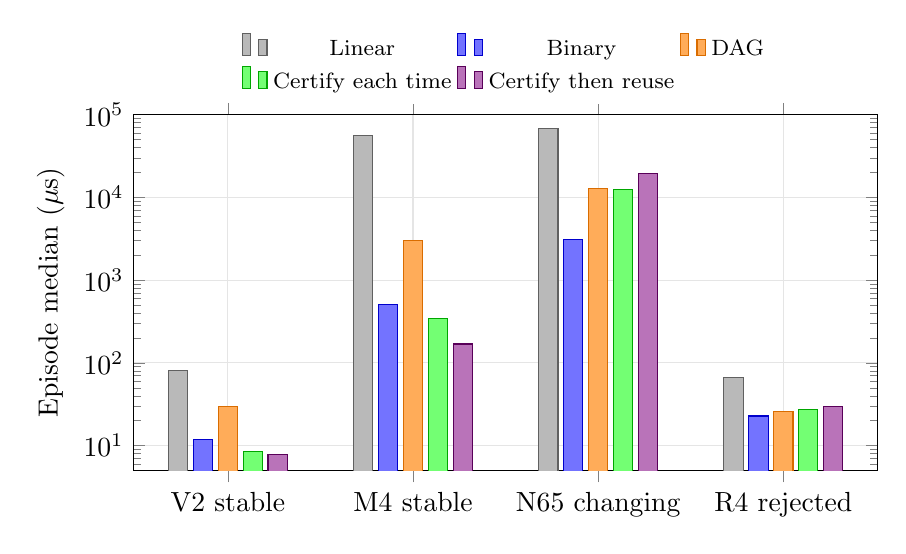
\begin{tikzpicture}
\begin{semilogyaxis}[
 width=.91\linewidth,height=6.1cm,
 ybar,bar width=7pt,enlarge x limits=.17,
 ymin=5,ymax=100000,
 xtick={1,2,3,4},xticklabels={V2 stable,M4 stable,N65 changing,R4 rejected},
 ylabel={Episode median (\(\mu\)s)},
 grid=major,grid style={gray!20},
 legend style={at={(.5,1.03)},anchor=south,legend columns=3,
 font=\footnotesize,draw=none,fill=white},
]
\addplot+[fill=gray!55,draw=gray!75!black,mark=none] coordinates
 {(1,80.939) (2,56700.377) (3,68078.844) (4,67.183)};
\addplot+[fill=blue!55,draw=blue!80!black,mark=none] coordinates
 {(1,11.810) (2,509.630) (3,3118.213) (4,22.804)};
\addplot+[fill=orange!65,draw=orange!85!black,mark=none] coordinates
 {(1,29.643) (2,2997.477) (3,12763.802) (4,25.643)};
\addplot+[fill=green!55,draw=green!65!black,mark=none] coordinates
 {(1,8.455) (2,347.091) (3,12401.246) (4,27.443)};
\addplot+[fill=violet!55,draw=violet!70!black,mark=none] coordinates
 {(1,7.857) (2,169.484) (3,19261.904) (4,29.486)};
\legend{Linear,Binary,DAG,Certify each time,Certify then reuse}
\end{semilogyaxis}
\end{tikzpicture}}
\caption{Five N04 routes on each fixture of Table~\ref{tab:n04smoke}. The logarithmic scale shows short and long episodes together; compare routes only \emph{within} a fixture. This fixed-order smoke test ran under Étendue3D interference.}
\label{fig:n04smoke}
\end{figure}

On V2, reused certification is about 1.5 times faster than binary powering. On M4, it is about 3 times faster and allocates about 4.2 times fewer bytes. On N65, coefficients change; binary powering is about 6.2 times faster than the reuse route and allocates about 10.3 times fewer bytes. On R4, a failed certification attempt adds work before exact fallback, and binary powering has the lowest median. These four fixtures do not define a routing threshold.

The one-thread collection used a fixed route order under Étendue3D load. Reverse order and an isolated rerun remain to be measured. Algebra and plan preparation differ among route contracts, so prepared states are not yet fully matched. The planned 30\,720-identity grid across twelve dimensions has not run. Checks include $\lambda=0$, changing inputs, and perturbations, but do not establish a general policy~\cite{n04smoke}.

\FloatBarrier

\subsection{Pfaffian for a scalar output}
\paragraph{Why consider it?}
Some applications request only the scalar coefficient of a long vector chain. Computing the complete multivector would build grades that are subsequently discarded. A Pfaffian can avoid that expansion, but its contraction cost and floating-point behavior must be compared with the work saved.

The expansion of Clifford products into contractions and Pfaffians goes back, in particular, to Wilmot~\cite{wilmotpf,wilmot2026}. For a \emph{symmetric} bilinear form, including a singular one, over a field of characteristic other than two, the scalar part of an \emph{ordered} product of $2m$ vectors is a signed sum over pairings. Set $K_{ij}=v_i\cdot v_j$ for $i<j$ and $K_{ji}=-K_{ij}$. Then
\[
 \langle v_1\cdots v_{2m}\rangle_0=\operatorname{Pf}(K).
\]
The orientation of $K$ comes from factor order; it is not obtained by antisymmetrizing a symmetric Gram matrix. The Clifford relation yields
\[
S(v_1,\ldots,v_{2m})=
\sum_{j=2}^{2m}(-1)^j(v_1\cdot v_j)
S(v_2,\ldots,\widehat v_j,\ldots,v_{2m}),
\]
with $S(\varnothing)=1$. This is the first-row Pfaffian expansion and requires no metric inverse. For four vectors it gives
$(v_1\!\cdot v_2)(v_3\!\cdot v_4)
-(v_1\!\cdot v_3)(v_2\!\cdot v_4)
+(v_1\!\cdot v_4)(v_2\!\cdot v_3)$.
A dense Pfaffian algorithm is cubic in $m$ after the contractions have been formed~\cite{wimmer}; expanding intermediate multivectors may be exponential. With $k=2m$ vectors of $n$ coordinates, the prototype forms dense contractions in $O(n^2k+nk^2)$ operations before $O(k^3)$ elimination. These costs can dominate when only a few axes are active.

This route returns only the requested scalar, not the full product. N05 checks signs with an independent rational oracle and rejects nonscalar outputs~\cite{n05report}. The numerical contract includes contraction conditioning: a rational identity does not guarantee an exact floating-point result. For multiple chains using a common vector pool, K3 shares contractions and buffers across scalar outputs, checking changes in the metric and coordinates~\cite{k3report}. It retains the same Pfaffian elimination and numerical limitation. Its plan, workspace, and validation costs determine whether sharing pays off; its experiment follows N05.

\paragraph{Test N05.}
\label{sec:n05perf}
The N05 prototype computes only $\langle v_1\cdots v_{2m}\rangle_0$, forming contractions and eliminating an antisymmetric matrix with pivoting~\cite{n05report}. This simple elimination does not implement Wimmer's optimized method. It passes 342/342 rational and contract tests for positive, signed, degenerate, null, and nonorthogonal symmetric metrics, including dimension 65. The independent oracle builds all grades through Chevalley's exterior action, without using a Pfaffian or Garamon multiplication. A one-thread PerfChecker smoke test qualifies 15/15 route cases over four fixtures and 225 observations under Étendue3D interference. Four routes with \emph{precomputed} contractions form a secondary category and are not compared to baselines that receive raw vectors.

Figure~\ref{fig:n05temps} uses the main output contract: each episode constructs N05 contractions, or the vectors and Garamon plan for a baseline, and retains the scalar from every iteration. Garamon's recursive route requests the scalar directly but is admitted here only for diagonal metrics; the complete-product route also materializes other grades. A comparable targeted-scalar baseline for general metrics is still missing. Chain lengths and horizons differ, so comparisons are meaningful \emph{within} each fixture, not between fixtures.

\begin{figure}[ht]
\centering
\IfFileExists{exploratory_n05temps.pdf}{\includegraphics[width=.92\linewidth]{exploratory_n05temps.pdf}}{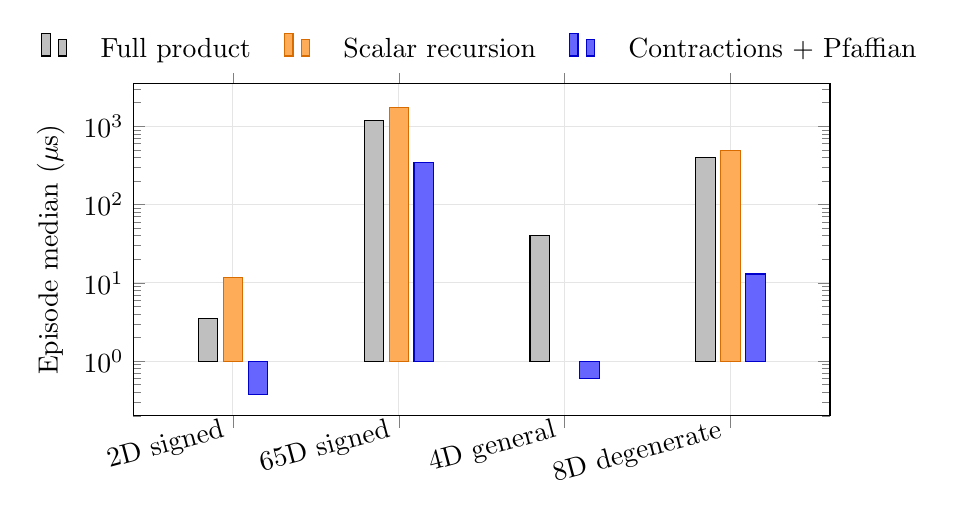
\begin{tikzpicture}
\begin{semilogyaxis}[
 width=.86\linewidth,height=5.8cm,
 ybar,bar width=7pt,enlarge x limits=.2,
 ymin=.2,ymax=3500,
 xtick={1,2,3,4},
 xticklabels={2D signed,65D signed,4D general,8D degenerate},
 x tick label style={rotate=15,anchor=east},
 ylabel={Episode median (\(\mu\)s)},
 grid=major,grid style={gray!20},
 legend style={at={(.5,1.03)},anchor=south,legend columns=3,column sep=10pt,draw=none,fill=white},
]
\addplot+[fill=gray!50,draw=black,mark=none] coordinates
 {(1,3.522) (2,1194.219) (3,40.469) (4,399.721)};
\addplot+[fill=orange!65,draw=orange!85!black,mark=none] coordinates
 {(1,11.565) (2,1729.413) (4,496.371)};
\addplot+[fill=blue!60,draw=blue!80!black,mark=none] coordinates
 {(1,.372) (2,342.305) (3,.595) (4,12.992)};
\legend{Full product,Scalar recursion,Contractions + Pfaffian}
\end{semilogyaxis}
\end{tikzpicture}}
\caption{Warm N05 smoke-test episodes. Chain lengths are $4,8,6,4$ and horizons $1,32,1,32$ in group order. The scale is logarithmic. The missing recursive bar in general 4D means \emph{nonadmission}, not zero time. Contraction construction is included; the full-product route has a different output contract.}
\label{fig:n05temps}
\end{figure}

The Pfaffian avoids producing unused grades in this scalar-only task, but establishes neither a threshold nor general superiority. Its exact algebraic identity does not ensure floating-point accuracy. With $G=\operatorname{diag}(1,1,-1)$ and $u=(1,2^{-30},1)$, the exact scalar is $\langle u^4\rangle_0=2^{-120}$. Forming \code{Float64} contractions and then evaluating the Pfaffian returns zero because $2^{-60}$ is lost in $1+2^{-60}-1$. The smoke test's absolute tolerance accepts zero and therefore cannot certify such small scalars. A numerical-precision policy, improved Gram construction, and isolated rerun are needed before selector admission. The 36\,480-identity manifest across dimensions 2--129 is prepared \emph{but has not run}.

\FloatBarrier
\paragraph{K3 experiment: share contractions between chains.}
\label{sec:k3perf}
When several ordered chains reuse vectors from one pool, K3 asks whether a shared contraction plan and workspace repay their preparation and validation costs. This N05 extension compares five organizations of the \emph{same} scalar Pfaffian calculation: independent chains, separate workspaces, sharing with repeated allocations, a common workspace, and a checked cache~\cite{k3report,k3protocol}. Each episode takes a metric, a vector pool, ordered chains, and horizon $H$, then returns an independently owned scalar matrix with one row per chain and one column per iteration. Pair planning, workspace construction, contractions, change checks, and output copies are included in episode time; no prepared artifact is free.

All 170 targeted tests pass. A one-thread PerfChecker smoke test qualifies 20/20 route cases, with 300 observations across four fixtures under Étendue3D interference. Figure~\ref{fig:k3partage} shows three of five routes; the other two, including repeated-allocation sharing, appear in the report. All five use the same elimination and are checked against a rational oracle under a declared \code{Float64} tolerance.

\begin{figure}[ht]
\centering
\IfFileExists{exploratory_k3partage.pdf}{\includegraphics[width=.92\linewidth]{exploratory_k3partage.pdf}}{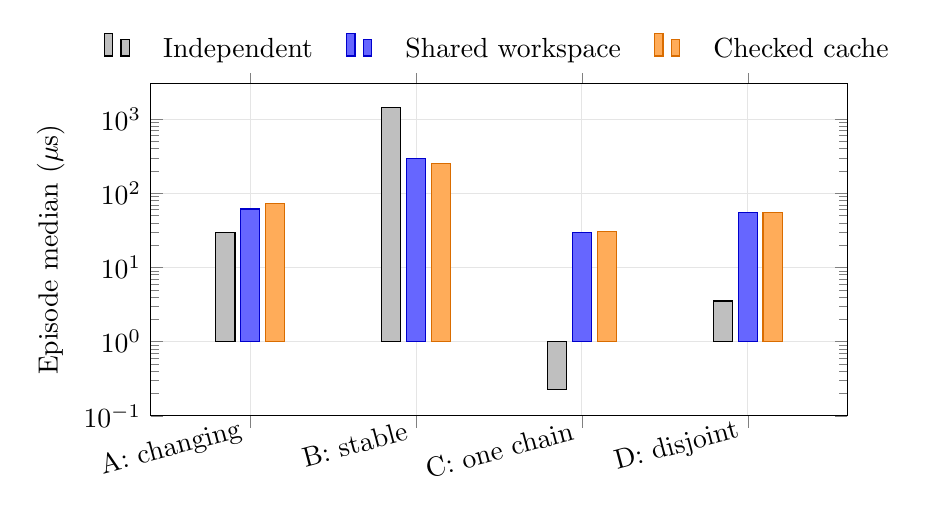
\begin{tikzpicture}
\begin{semilogyaxis}[
 width=.86\linewidth,height=5.8cm,
 ybar,bar width=7pt,enlarge x limits=.2,
 ymin=.1,ymax=3000,
 xtick={1,2,3,4},
 xticklabels={A: changing,B: stable,C: one chain,D: disjoint},
 x tick label style={rotate=15,anchor=east},
 ylabel={Episode median (\(\mu\)s)},
 grid=major,grid style={gray!20},
 legend style={at={(.5,1.03)},anchor=south,legend columns=3,column sep=10pt,draw=none,fill=white},
]
\addplot+[fill=gray!50,draw=black,mark=none] coordinates
 {(1,29.708) (2,1425.417) (3,.229) (4,3.536)};
\addplot+[fill=blue!60,draw=blue!80!black,mark=none] coordinates
 {(1,61.315) (2,297.041) (3,29.993) (4,55.511)};
\addplot+[fill=orange!65,draw=orange!85!black,mark=none] coordinates
 {(1,72.010) (2,253.998) (3,30.725) (4,55.416)};
\legend{Independent,Shared workspace,Checked cache}
\end{semilogyaxis}
\end{tikzpicture}}
\caption{K3 total warm cost, including preparation and an owned output, on a logarithmic scale. A: 4D, four changing chains, $H=32$; B: 65D, four stable chains, $H=32$; C: 4D, one chain, $H=1$; D: general 4D, four disjoint chains, $H=3$. Compare routes only \emph{within} a fixture. This exploratory smoke test establishes no threshold.}
\label{fig:k3partage}
\end{figure}

In fixture B, medians are 1\,425.417~\(\mu\)s for independent chains, 297.041~\(\mu\)s for a shared workspace, and 253.998~\(\mu\)s for a checked cache. A separate diagnostic replay counts 128, 32, and one contraction construction respectively; these counts are not added to measured time. In fixture A, changing inputs require 32 reconstructions and the shared workspace loses, 61.315 versus 29.708~\(\mu\)s. In fixture C, sharing a single short chain costs nearly 30~\(\mu\)s versus 0.229~\(\mu\)s independently. Reducing contraction count therefore does not guarantee a faster episode. Sharing also does not fix N05's \code{Float64} cancellation: the $2^{-120}$ counterexample still returns zero.

\paragraph{Audited selective screen.}
A separate screen compares independent chains with a shared workspace under identical independently owned outputs, including preparation and checks. It qualifies 176/176 unique identities in eleven dimensions from 2 to 129, horizons one and 32, stable or changing inputs, and two route orders~\cite{k3screen}. The audit verifies case coverage and the rational oracle. Five cases from the first pass were repeated during recovery; all 2\,715 raw samples remain archived, but those duplicates are excluded from the selected 2\,640 samples and 176 cases. Each of the 88 timing pairs compares routes \emph{within one pass}.

\begin{table}[ht]
\centering\small
\begin{tabular}{@{}lrrr@{}}
\toprule
Pass & Pairs & Workspace faster & Fewer allocated bytes \\
\midrule
Initial & 64 & 12 & 40 \\
Rerun & 24 & 20 & 24 \\
\bottomrule
\end{tabular}
\caption{K3 selective screen under Julia 1.13. Passes cover different dimension subsets, so their counts are not pooled into a global win frequency. One thread and concurrent Étendue3D load~\cite{k3screen}.}
\label{tab:k3screen}
\end{table}

At 2D, $H=1$, stable inputs, and direct route order, the independent episode takes 0.968~\(\mu\)s versus 52.146~\(\mu\)s for the workspace. At 129D, $H=32$ with stable inputs and direct order, medians are 4\,745.279 and 828.971~\(\mu\)s, with 20\,339\,824 and 178\,592 allocated bytes per episode respectively. Chains activate at most four directions and reuse a small vector pool, so ambient dimension alone does not explain these contrasts. At 65D and $H=32$ with changing inputs, route rankings vary with order, particularly as the independent baseline slows. This anomaly needs an isolated rerun before causal interpretation or a threshold.

The first pass exceeded its nominal time window by about 12 seconds; recovery completed within its 900-second limit. Of 440 selective-grid identities, 264 have not run, and the separate 25\,920-identity replay manifest also remains unexecuted. All five routes, floating-point accuracy, and route orders need comparison on an idle machine before automatic selection.

\FloatBarrier
\subsection{Rank of the cross-Gram matrix}
\paragraph{Why consider it?}
Products of decomposable blades can be described through contractions and angles between subspaces~\cite{mandolesi}. For $A=a_1\wedge\cdots\wedge a_p$ and $B=b_1\wedge\cdots\wedge b_q$, form the cross-Gram matrix $C_{ij}=a_i\cdot b_j$. Contraction terms of order $k$ involve $k\times k$ minors of $C$. If its rank is certified as $\rho$, these minors vanish for $k>\rho$. A suitable contraction decomposition could then omit some grades \emph{without approximation}.

\paragraph{Proposed experiment; no Garamon measurements.}
The filter must be proved for the implemented product convention. A test should compare low-rank and full-rank cross-Gram matrices with matched blades, metrics, and outputs, while charging factorization cost. An SVD threshold in floating-point arithmetic makes an approximate rank decision; exact omission requires rank certification over the chosen coefficient domain.

\subsection{Gaussian fermionic states}
\paragraph{Why consider it?}
Gaussian fermionic states retain compact descriptions under certain quadratic transformations~\cite{bravyigaussian}. This suggests a closed representation for chains of Majorana operations, with expansion only for requested outputs. Non-Gaussian simulations also require tracking phases and departures from that closed class~\cite{dias}. Two operators with the same conjugation action on vectors can still differ by a sign relevant to an amplitude.

\paragraph{Proposed experiment; no Garamon measurements.}
A possible gain concerns long chains that remain in this closed family, not arbitrary multivectors. A trial should check amplitudes and signs against a complete oracle on small cases, then add a controlled number of non-Gaussian operations. It must record representation growth and final-conversion cost.

\subsection{Factorized change of basis}
\paragraph{Why consider it?}
A linear map $Q$ on vectors induces $\Lambda^k Q$ on grade $k$, a matrix of size $\binom nk\times\binom nk$. Orbital rotations can instead be applied as a sequence of Givens rotations to relevant coefficients, avoiding that full matrix~\cite{ffsim}. Factoring an orthogonal $Q$ into $O(n^2)$ rotations gives up to order $n^2\binom nk$ elementary operations in the dense case; conversion and memory access still count.

\paragraph{Proposed experiment; no Garamon measurements.}
The target is repeated basis changes at grades where constructing or storing the induced matrix dominates cost. A benchmark should compare factorized application, explicit induced matrices, and computation in the original basis, using a coefficient oracle and peak-memory measurement. Support fill-in can make factorization slower. Nonorthogonal transformations need their own factorization and complete cost accounting.

\subsection{Signed disjoint convolution}
\paragraph{Why consider it?}
In the outer algebra, the $S$ mask coefficient of the product is \[
 (a\wedge b)_S=
 \sum_{\substack{A\sqcup B=S}}(-1)^{\operatorname{inv}(A,B)}a_A b_B.
\] A direct dense sum visits on the order of $3^n$ disjoint pairs. Włodarczyk gives a \emph{signed} disjoint convolution in $O^*(2^{\omega n/2})$ within its algebraic model~\cite{wlodarczyk}; dropping the sign would compute a different product. This asymptotic bound does not establish practical constants, memory use, or behavior for sparse supports and floating-point coefficients.

\paragraph{Proposed experiment; no Garamon measurements.}
A test should cover moderately sized, fairly dense exterior products over an admissible coefficient domain. It should compare time and memory against sparse traversal and full enumeration, with every coefficient checked. Large auxiliary tables and additions may erase the asymptotic gain.

\subsection{Bilinear synthesis of small kernels}
\paragraph{Why consider it?}
A fixed product has a bilinear tensor $c_k=\sum_{ij}T_{kij}a_i b_j$. A decomposition $c=W((Ua)\odot(Vb))$ can share multiplications across outputs. AlphaTensor found such decompositions for matrix multiplication, a related problem~\cite{alphatensor}. For Garamon, the proposal is \emph{offline} synthesis of small fixed kernels, followed by exact verification against the product tensor. Multiplication count alone does not predict addition count, code size, or floating-point stability.

\paragraph{Proposed experiment; no Garamon measurements.}
Candidate kernels must be compared with existing generation at bounded dimensions and grades, including generation, compilation, and execution. Equivalence must be proved over the target coefficient domain; an identity modulo one prime does not automatically hold over $\mathbb R$.

\subsection{Verified superoptimization}
\paragraph{Why consider it?}
After selecting a traversal, a product may still repeat a short sequence millions of times: compute the sign of a blade pair, their XOR and intersection, and the output address. Verified superoptimization targets \emph{this local instruction cost}. It searches for a different instruction sequence implementing the same function and proves equivalence for the admitted integer types and edge cases. It does not change which supports are traversed or which outputs are requested. Its value must therefore be measured per call of the \emph{same} kernel after the representation and high-level algorithm are fixed.

Minotaur synthesizes SIMD sequences and checks semantic equivalence with Alive2~\cite{minotaur}; AlphaEvolve explores programs by another method~\cite{alphaevolve}. They motivate examining small sign, XOR, intersection, and accumulation loops. The possible gain concerns instructions, loads, and registers, not a reduction in the number of blade products.

\paragraph{Proposed experiment; no Garamon speed result.}
Compare the current loop with a candidate receiving identical masks, metrics, and coefficients and returning identical outputs. First prove equivalence of the integer portion for the types, overflow behavior, and compiler settings in use. Reassociation or fusion of floating-point accumulations can change result bits, so that contract needs separate verification. Then measure first compilation, warm execution, allocations, and code size on several architectures, with the same traversal strategy on both sides. No Garamon superoptimized candidate has yet been validated or timed; no figure in this article assigns a speedup to it.

\subsection{Active-front scheduling}
\paragraph{Why consider it?}
Wavefront path tracing groups active paths to reduce GPU divergence~\cite{lainewavefront}. An irregular product recursion could similarly form prefix frontiers, discard branches proven zero, and group survivors by grade or destination. This changes scheduling and locality without changing the arithmetic identity.

\paragraph{Proposed experiment; no Garamon measurements.}
The plausible workload is a large batch of products sharing transitions. A test should compare direct recursion with frontier scheduling on CPU, then on GPU if batch size warrants it. Frontier storage, transfers, synchronization, and floating-point summation order are costs and risks; a small sparse task may lose.

\subsection{Radix index for materialized supports}
\paragraph{Why consider it?}
Adaptive radix trees index stored keys with compact navigation~\cite{art}. They might accelerate repeated queries against a \emph{materialized} support mask set. This differs from Garamon C++'s virtual recursion tree, which need not store index nodes for active masks.

\paragraph{Proposed experiment; no Garamon measurements.}
A test should compare radix trees, sorted arrays, hash tables, and ZDDs for lookup, intersection, and iteration on identical supports, including construction, retained memory, locality, and updates. Unreused random supports provide a negative case. A one-off product cannot amortize an index without a measured benefit.

\Needspace{13\baselineskip}
\subsection{Exact multimodular arithmetic}
\paragraph{Why consider it?}
Correctness tests can themselves become expensive when their oracle multiplies very large integers or rational numbers to check every coefficient. Exact multimodular arithmetic addresses this \emph{coefficient arithmetic}. Binary ranking instead reduces the number of possible \emph{masks}; verified superoptimization reduces instructions inside one loop. The multimodular approach computes several small modular results and reconstructs a large exact result. It could speed up an oracle or repeated integer product when modular computation plus reconstruction costs less than direct \code{BigInt} arithmetic. It does not target ordinary \code{Float64} products.

FLINT supplies simultaneous modular reduction and Chinese-remainder reconstruction with reusable preprocessing~\cite{flintcrt}. For sufficiently large integer or rational coefficients, one could compute modulo several primes and reconstruct each coefficient. If the product of moduli exceeds twice a certified absolute bound, signed reconstruction identifies the exact integer. A nonzero residue proves a coefficient nonzero; zero residues modulo only a few primes do \emph{not} prove that it is zero.

\paragraph{Proposed experiment; no Garamon speed result.}
The baseline will compute identical symbolic oracles, inverses, and large-coefficient products directly with \code{BigInt} or rational arithmetic. The candidate must pay for every modular reduction, modular product, and Chinese-remainder reconstruction. Certified bounds on coefficients and denominators, together with treatment of bad primes, are required for exact equality. We would compare \emph{total} time and memory on identical inputs over several coefficient sizes to locate any amortization point. No Garamon multimodular prototype has been timed; results in the other figures do not establish a gain for this technique.

\subsection{Filtered geometric predicates}
\paragraph{Why consider it?}
CGAL combines approximate evaluation, an error bound, and exact fallback when a sign remains uncertain~\cite{cgalfiltered}. A Garamon API asking only for the sign of an orientation or comparison could use the same pattern: return early when an interval excludes zero; otherwise compute an exact decision. Correctness is relative to the exact representation of the inputs.

\paragraph{Proposed experiment; no Garamon measurements.}
The test must distinguish decisions far from zero from nearly degenerate cases, and record fallback frequency and cost. It must specify how intermediate values and coordinates are constructed. An exact predicate answers its stated decision question; it does not replace a complete multivector output or turn a tolerance-based calculation into an exact one.

\paragraph{Structural admission.}
These routes assume certificates attached to objects or plans: binary rank, sector, radical, minimal polynomial, decomposability, Gram rank, or coefficient bound. A certificate is established once, propagated only through proven rules, and invalidated by an unsupported operation. The $2^d$ bound illustrates a potentially large reduction, but measurements must include certification and conversion costs. Compatibility with Garamon's public contract remains an open question. A separate matrix inventories 46 technique families and 1\,035 pairs with proposed conditions and tests~\cite{compatmatrix}; it contains no new timings or measured combined gain.

\section{Discussion and experimental tracks}
The methods do not form a single hierarchy. Sparse program planning~\cite{galley}, reusable workspaces~\cite{sparseworkspace}, joins~\cite{leapfrog}, and equality saturation~\cite{egg} suggest complementary ideas. Their adoption in Garamon requires correctness proofs and measurements on Garamon workloads. The following questions remain open:
\begin{enumerate}
\item Compare sparse accumulation, dense buffers with touched positions, sorted merging, grade blocks, and products of four or more factors. Measure preparation, conversion, JIT, execution, and peak memory, including long chains with changing supports.
\item Separate preprocessing, first compilation, and the native process cache. If a finite catalog of common algebras is precompiled, also test discovery of previously unseen metrics and supports. Charge catalog or application-image construction to the sessions it is intended to serve.
\item Extend the exact four-thread packed comparison to other CPU thread counts and separate processes on independent products and batches. Share immutable plans, give each task its own workspace, and count startup, scheduling, serialization, duplicated memory, and contention. GPU comparisons must also include transfer, launch, synchronization, VRAM, and the output destination. Four CPU threads change the per-product-host-output crossover; the separate resident-sum contract changes it again. The fused-kernel and CUDA Graph pilots test distinct ways to reduce submission cost, with the graph measured only on repeated identical-value sums. None supplies an automatic threshold.
\item Extend the contextual portfolio from an analytical rule and cost table to a learned model only after sufficient independent cases exist. Keep algebra and support families separate between training and testing. SHAP values~\cite{shap} may explain model predictions, but do not prove their cause or performance. Measure regret against the best retrospective choice, selector overhead, and first-call quality.
\end{enumerate}

An \emph{approximate} pruning experiment can omit a contribution, log it, and correct it later. For an affine recurrence with $x_{t+1}=L_tx_t+b_t$ and $\widehat{x}_{t+1}=L_t\widehat{x}_t+b_t-d_t$, the error $e_t=x_t-\widehat{x}_t$ satisfies
\begin{equation}
e_{t+1}=L_t e_t+d_t.
\label{eq:recurrence}
\end{equation}
The recurrence does not reconstruct omitted terms on its own. One must carry their residual, bound its influence, or replay a segment from an exact state. Nonlinear recurrences add cross terms that complicate correction. Roulette over telescoping corrections can be unbiased under stated conditions~\cite{rhee}, but a single realization need not yield an exact trajectory. Future comparisons must distinguish rational equality, bitwise floating-point equality, certified error bounds, and observed error. Certificates, logs, and replay count toward total cost. An approximate route requires an explicit error contract and cannot silently replace exact computation.

\section{Validity limits and reproducibility}
Campaigns cover distinct domains and budgets. Fixed sparse support can remain computable as $n$ grows, so there is no universal maximum dimension. The scan up to 256D does not cover all metrics or long expressions. Workspace measurements focus on a Euclidean metric and immediately consumed results. The 10\,000-call times have only one sample per case. The \code{UInt128}/\code{BigInt} comparison isolates a simplified kernel. The pruning experiment uses at most four active directions and does not represent the public kernel. The I15.6 campaign measures native-cache reuse after restart for one EGA3 catalog and twelve 4D contexts; it does not qualify a production catalog or another machine. The first TripleJoin campaign uses only two to four active directions, and some long-horizon cases have one timing sample. Concurrent Étendue3D processes affected CPU availability and frequency. All speed rankings in this version are exploratory; an isolated full rerun is needed before choosing thresholds.

N01 was evaluated on one thread and in two orders under the same interference. Its 648 cases are timed complete episodes; the 10\,287 cases of its extended manifest have not run. The separate K1v2 replay qualified only its first size-two batch, 324 of 41\,148 cases; the remaining batches have not run.

N03 has two corrected screens of 756 cases each across twelve dimensions and reverse route orders. Concurrent load, small active supports, and order-sensitive rankings prevent a speed threshold. JIT diagnostics from a shared process do not measure cold-start cost. The initial run rejected because of a generator error remains archived and is excluded from the 1\,512 qualified cases.

N05 covers four vector-chain fixtures and a scalar output. Contraction construction is timed, but a comparable scalar-only baseline for general metrics and a floating-point accuracy policy are still missing. Its 36\,480 planned replay identities have not run.

K3 has four five-route smoke fixtures, followed by an audited selective screen of 176 unique identities across eleven dimensions and two routes. The first pass exceeded its planned time window by about 12 seconds; five affected cases were excluded from comparison. The remaining 264 selective identities, 25\,920 full-grid identities, three other routes, and tests on poorly conditioned inputs remain open. N04 passes its rational assertions under Julia 1.13, and its first smoke test qualifies 20/20 cases with 300 observations in one order under Étendue3D interference. Preparation differs among routes, and its 30\,720-identity grid has not been measured. The third B1 batch qualifies 96 episodes of 1 to 1\,024 products with 2\,016 observations under the same interference. Its supports contain only four masks. Later B1W preflights test a different workspace contract; the B1 batch alone does not establish a general bounds-checking policy.

While Étendue3D shares the machine, further screening will use at most four threads or workers, usually one. The larger case matrix needs a coordinated rerun on an otherwise idle machine, with identical contracts and retained observations.

The paired C++/Julia benchmark covers only the packed product in two algebras, two support sets, and four reuse horizons. The first pass did not retain its 31 individual samples; only summary statistics and oracle results remain. The two later, separate order-reversed campaigns retain 31 raw warm samples per case and pass the same exact qualification. The upstream C++ route is descriptive and is not a fourth matched route.
\paragraph{Compilation options and bounds checks.}
The matched C++ packed kernel uses Clang with \code{-O2}, \code{-march=native}, and \code{-ffp-contract=off}; this host lacks \code{g++}. The Julia 1.13 \code{run\_packed\_batch} loop already uses \code{@inbounds}. The difference between these kernels therefore cannot be attributed to removing Julia bounds checks on this evidence, or to an untested C++ code-generation change~\cite{boundsreport}.

A B1 driver under \code{perf/}, without changes to the public kernel, compares checked buffered accumulation with a variant annotated by \code{@inbounds}. Each call copies masks and paths into private vectors and validates algebra, supports, sizes, and index bounds. Only accumulation over those private buffers skips bounds checks. Both routes pay for the same copying and validation. Under Julia 1.13, the targeted suite passes 550/550 tests with \code{--check-bounds=yes} and again with \code{--check-bounds=auto}~\cite{boundsreport}.

\paragraph{First smoke B1: specialized code and full time.}
Under Julia 1.13, a first trial PerfChecker qualifies 8/8 cases in Euclidean 8D with small support and $H=1$. Two distinct processes employ \code{--check-bounds=yes} or \code{auto} , with \code{-O2} , \code{--cpu-target=native} and a thread. Each process passes the checked and annotated routes in both orders. The three phases --- plan construction, hot calculation with reused plan, and complete episode with reconstructed plan and independent owned output --- each have seven observations per case: 168 observations in total. The episode is timed directly and the entire independent oracle checks the outputs~\cite{b1smoke} .

\begin{table}[ht]
\centering\small
\begin{tabular}{@{}llrr@{}}
\toprule
Bounds & Route & Order 1: warm / episode & Order 2: warm / episode \\
\midrule
\code{yes} & Checked & 1.122 / 6.361 & 0.867 / 6.256 \\
\code{yes} & Annotated & 0.977 / 6.442 & 0.901 / 6.320 \\
\code{auto} & Checked & 0.887 / 7.331 & 0.941 / 6.120 \\
\code{auto} & Annotated & 0.840 / 6.915 & 0.857 / 6.263 \\
\bottomrule
\end{tabular}
\caption{First B1 smoke test: medians in microseconds from seven observations per phase and case. Warm execution reuses the plan; a complete episode rebuilds it. Two orders were separate passes under Étendue3D interference. Raw samples and provenance: \cite{b1smoke}.}
\label{tab:b1smoke}
\end{table}

Both routes allocate 3\,536 bytes in 42 allocations during the warm phase and 12\,640 bytes in 221 allocations per complete episode; construction alone accounts for 9\,104 bytes in 179 allocations. Under \code{--check-bounds=auto}, specialized LLVM IR for checked accumulation contains a \code{throw\_boundserror} path absent from annotated accumulation. Under forced checks, that path appears in both. The intended local code difference is therefore present, but this does not prove that all bounds checks in the complete product disappear. Warm differences do not translate into a stable complete-episode gain. Route order, seven observations per phase, and Étendue3D load prevent a production recommendation~\cite{b1smoke}.

\paragraph{Preflight B1: 12 ambient dimensions.}
The first smoke test covers only 8D. A subsequent scan asks whether its warm contrast persists across ambient dimensions and across the 64D mask-representation boundary. It qualifies 48/48 cases over the twelve dimensions in Table~\ref{tab:b1dimensions}: checked and annotated routes in two orders per dimension. Each dimension uses a fresh Julia 1.13 process with automatic bounds checks, \code{-O2}, native target, one thread, positive metric, low-grade support, and $H=1$. Seven observations per case and phase cover construction, warm computation, and complete episodes, for 1\,008 raw observations. An exact oracle checks independently owned outputs~\cite{b1dimensions}.

\begin{table}[ht]
\centering\footnotesize
\begin{tabular}{@{}rrrrrrr@{}}
\toprule
$n$ & Warm V & Warm A & Episode V & Episode A & Warm bytes & Episode bytes \\
\midrule
2 & 0.810 & 0.828 & 9.470 & 6.285 & 3\,536 & 12\,496 \\
3 & 0.831 & 0.796 & 6.151 & 6.162 & 3\,536 & 12\,496 \\
4 & 1.008 & 0.821 & 6.094 & 5.989 & 3\,536 & 12\,544 \\
6 & 0.860 & 0.802 & 6.627 & 6.359 & 3\,536 & 12\,592 \\
8 & 0.864 & 0.824 & 6.520 & 6.533 & 3\,536 & 12\,640 \\
12 & 0.869 & 0.825 & 6.347 & 6.483 & 3\,536 & 12\,736 \\
16 & 0.879 & 0.819 & 6.378 & 6.341 & 3\,536 & 12\,832 \\
32 & 0.888 & 0.822 & 6.629 & 6.311 & 3\,536 & 13\,216 \\
64 & 0.972 & 0.921 & 6.569 & 6.393 & 3\,536 & 13\,984 \\
65 & 1.125 & 1.175 & 7.316 & 7.172 & 4\,384 & 17\,312 \\
96 & 1.124 & 1.150 & 7.550 & 7.185 & 4\,384 & 18\,128 \\
128 & 1.129 & 1.051 & 7.280 & 7.617 & 4\,384 & 18\,944 \\
\bottomrule
\end{tabular}
\caption{B1 dimension preflight: medians in microseconds across two passes, 14 observations per route and phase. V is checked and A is annotated. A complete episode rebuilds the plan and retains its owned output. Allocated bytes match between routes. Native data: \cite{b1dimensions}.}
\label{tab:b1dimensions}
\end{table}

\begin{figure}[ht]
\centering
\IfFileExists{exploratory_b1dimensions.pdf}{\includegraphics[width=.92\linewidth]{exploratory_b1dimensions.pdf}}{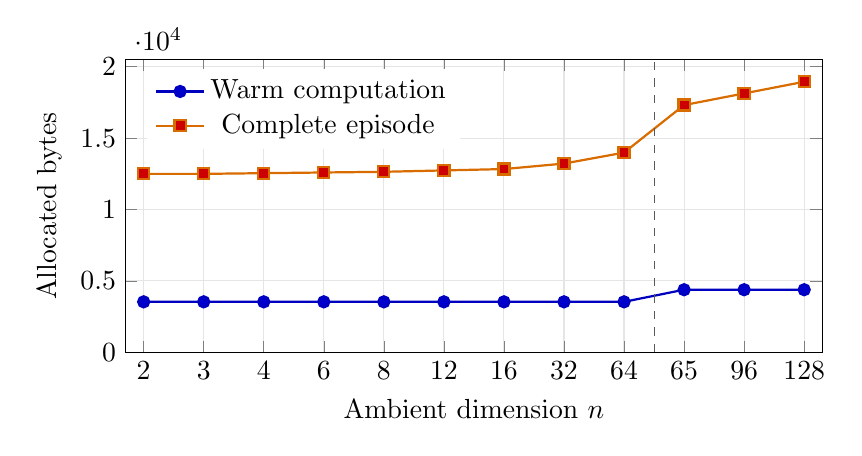
\begin{tikzpicture}
\begin{axis}[
 width=.86\linewidth,height=5.3cm,
 xmin=.7,xmax=12.3,ymin=0,ymax=20500,
 xtick={1,2,3,4,5,6,7,8,9,10,11,12},
 xticklabels={2,3,4,6,8,12,16,32,64,65,96,128},
 xlabel={Ambient dimension $n$},ylabel={Allocated bytes},
 grid=major,grid style={gray!20},
 legend style={at={(.03,.97)},anchor=north west,draw=none,fill=white},
]
\addplot+[blue!75!black,thick,mark=*] coordinates
 {(1,3536) (2,3536) (3,3536) (4,3536) (5,3536) (6,3536)
  (7,3536) (8,3536) (9,3536) (10,4384) (11,4384) (12,4384)};
\addplot+[orange!85!black,thick,mark=square*] coordinates
 {(1,12496) (2,12496) (3,12544) (4,12592) (5,12640) (6,12736)
  (7,12832) (8,13216) (9,13984) (10,17312) (11,18128) (12,18944)};
\draw[dashed,gray!70!black] (axis cs:9.5,0) -- (axis cs:9.5,20500);
\legend{Warm computation,Complete episode}
\end{axis}
\end{tikzpicture}}
\caption{Allocated bytes in the two B1 routes, identical in each case. The dotted line marks the 64D-to-65D switch from \code{UInt64} to \code{UInt128}. Input masks remain $0,1,2,3$; the graph does not measure dense support growth~\cite{b1dimensions}.}
\label{fig:b1dimensions}
\end{figure}
\FloatBarrier

Warm computation makes 42 allocations for each route and dimension. A complete episode makes 221 allocations through 64D and 273 from 65D. The allocation change at 65D coincides with the switch from \code{UInt64} to \code{UInt128} masks. The four input masks remain $0,1,2,3$, so only two basis directions are active regardless of ambient dimension. This scan primarily varies algebra metadata and mask type; high grades and dense supports are outside its scope.

For 2D checked execution, the second pass has a complete-episode median of 10.874~\(\mu\)s versus 6.149~\(\mu\)s in the first, while warm medians are nearly identical at 0.811 and 0.809~\(\mu\)s. The pooled 9.470~\(\mu\)s episode median therefore cannot identify a causal bounds-checking effect. Episodes are nearly tied at 8D, and checked execution has the lower median at 128D. Under Étendue3D interference, these 48 cases establish neither a threshold nor a default setting, and they do not compare C++~\cite{b1dimensions}.

\paragraph{Preflight B1: high-grade blades.}
A second batch tests higher-grade support: its four masks are $0,1,2^n-1,2^n-2$. The last two have grades $n$ and $n-1$, while the number of terms and product paths remains small. It uses the same twelve dimensions, automatic bounds checks, \code{-O2}, native target, positive metric, $H=1$, one thread, and two route orders. It qualifies 48/48 cases with seven observations in each of three phases per case, for 1\,008 raw observations; an exact oracle verifies owned outputs. Together, the two B1 dimension scans comprise 96 cases and 2\,016 observations~\cite{b1highgrade}.

\begin{table}[ht]
\centering\footnotesize
\begin{tabular}{@{}rrrrrr@{}}
\toprule
$n$ & Warm V & Warm A & Episode V & Episode A & Episode bytes \\
\midrule
2 & 0.825 & 0.760 & 6.173 & 6.463 & 12\,496 \\
3 & 1.123 & 0.784 & 6.883 & 6.602 & 12\,496 \\
4 & 0.792 & 0.840 & 6.265 & 6.096 & 13\,024 \\
6 & 0.770 & 0.778 & 6.796 & 6.389 & 13\,744 \\
8 & 0.762 & 0.803 & 6.306 & 6.611 & 13\,792 \\
12 & 0.786 & 0.762 & 8.101 & 7.003 & 17\,888 \\
16 & 0.810 & 0.790 & 6.893 & 7.540 & 17\,984 \\
32 & 0.849 & 0.812 & 7.133 & 6.907 & 18\,368 \\
64 & 0.890 & 0.885 & 8.359 & 8.220 & 33\,152 \\
65 & 1.153 & 1.240 & 10.611 & 10.300 & 36\,128 \\
96 & 1.191 & 1.160 & 11.265 & 11.591 & 36\,944 \\
128 & 1.260 & 1.196 & 12.735 & 12.160 & 37\,760 \\
\bottomrule
\end{tabular}
\caption{B1 high-grade preflight: medians in microseconds from 14 observations per route and phase, two passes of seven. V is checked; A is annotated. A complete episode includes plan construction and one owned output; allocated bytes match between V and A. Native data: \cite{b1highgrade}.}
\label{tab:b1highgrade}
\end{table}

\begin{figure}[ht]
\centering
\IfFileExists{exploratory_b1gradealloc.pdf}{\includegraphics[width=.92\linewidth]{exploratory_b1gradealloc.pdf}}{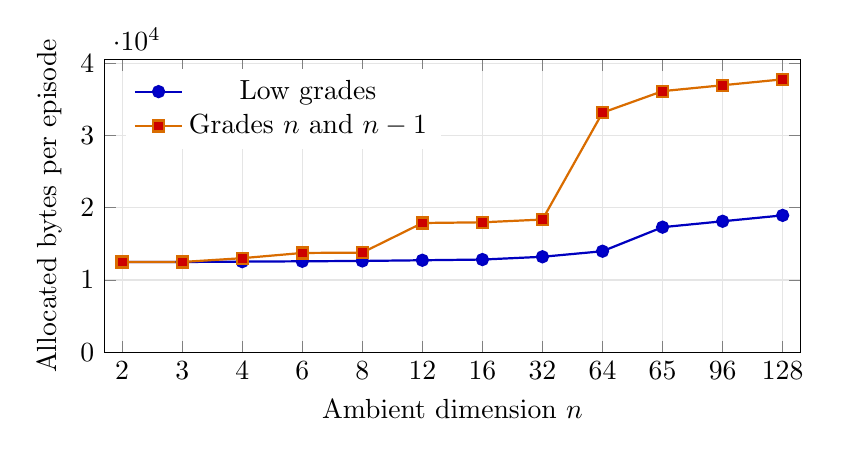
\begin{tikzpicture}
\begin{axis}[
 width=.86\linewidth,height=5.3cm,
 xmin=.7,xmax=12.3,ymin=0,ymax=40500,
 xtick={1,2,3,4,5,6,7,8,9,10,11,12},
 xticklabels={2,3,4,6,8,12,16,32,64,65,96,128},
 xlabel={Ambient dimension $n$},ylabel={Allocated bytes per episode},
 grid=major,grid style={gray!20},
 legend style={at={(.03,.97)},anchor=north west,draw=none,fill=white},
]
\addplot+[blue!75!black,thick,mark=*] coordinates
 {(1,12496) (2,12496) (3,12544) (4,12592) (5,12640) (6,12736)
  (7,12832) (8,13216) (9,13984) (10,17312) (11,18128) (12,18944)};
\addplot+[orange!85!black,thick,mark=square*] coordinates
 {(1,12496) (2,12496) (3,13024) (4,13744) (5,13792) (6,17888)
  (7,17984) (8,18368) (9,33152) (10,36128) (11,36944) (12,37760)};
\legend{Low grades,Grades $n$ and $n-1$}
\end{axis}
\end{tikzpicture}}
\caption{Allocations per complete B1 episode in two successive batches. Checked and annotated routes match at fixed dimension and support. Both batches ran alongside Étendue3D; their descriptive difference alone cannot attribute all extra cost to grade~\cite{b1dimensions,b1highgrade}.}
\label{fig:b1gradealloc}
\end{figure}
\FloatBarrier

Warm computation allocates 3\,536 bytes in 42 allocations through 64D, and 4\,384 bytes in 42 allocations from 65D, as in the low-grade batch. High-grade complete episodes rise from 221 allocations in 2--3D to 279 in 64D and 309 in 65D. Most additional bytes arise during plan construction; accumulation over four terms remains short. Checked episodes are faster at 8D, annotated ones at 12D, and the ranking changes again at 16D and 96D. No uniform advantage appears. The low- and high-grade batches ran successively under Étendue3D interference. Matching settings do not make their timing difference a clean estimate of grade alone. Preparation profiling and an isolated rerun are needed before a selection rule~\cite{b1highgrade}.
\FloatBarrier

\paragraph{B1 preflight: episodes from one to 1\,024 products.}
\emph{Why a third experiment?} The preceding two batches measured $H=1$ and could not show whether a small warm-kernel difference accumulates when supports remain stable. This batch compares checked and annotated routes over complete episodes with $H=1,32,1\,024$. It counts one plan construction, per-product validation and private copies, and retention of all independently owned outputs. The 96/96 qualified cases cross dimensions 2, 8, 65, and 128 with low- and high-grade supports, two routes, and two orders. Settings are Julia 1.13, \code{--check-bounds=auto}, \code{-O2}, native CPU, positive metric, and one thread. Seven observations per phase and case yield 2\,016 raw observations. An exact oracle verifies all $H$ owned outputs before and after measurement. Concurrent Étendue3D load makes timing comparisons exploratory~\cite{b1horizons}.

\begin{table}[ht]
\centering\small
\begin{tabular}{@{}rlrrrrr@{}}
\toprule
$n$ & Support & $H$ & V (\(\mu\)s) & A (\(\mu\)s) & Bytes & Alloc. \\
\midrule
2 & low & 1 & 6.395 & 6.242 & 12\,496 & 221 \\
2 & low & 32 & 24.383 & 23.586 & 114\,736 & 1\,399 \\
2 & low & 1\,024 & 602.234 & 580.655 & 3\,384\,312 & 39\,096 \\
2 & high & 1 & 6.862 & 6.796 & 12\,496 & 221 \\
2 & high & 32 & 24.969 & 23.578 & 114\,736 & 1\,399 \\
2 & high & 1\,024 & 585.426 & 581.638 & 3\,384\,312 & 39\,096 \\
8 & low & 1 & 6.797 & 6.444 & 12\,640 & 221 \\
8 & low & 32 & 24.183 & 25.011 & 114\,880 & 1\,399 \\
8 & low & 1\,024 & 628.263 & 613.279 & 3\,384\,456 & 39\,096 \\
8 & high & 1 & 7.158 & 6.698 & 13\,792 & 233 \\
8 & high & 32 & 25.785 & 25.227 & 116\,032 & 1\,411 \\
8 & high & 1\,024 & 624.698 & 631.071 & 3\,385\,608 & 39\,108 \\
65 & low & 1 & 7.223 & 7.037 & 17\,312 & 273 \\
65 & low & 32 & 32.215 & 33.181 & 145\,840 & 1\,451 \\
65 & low & 1\,024 & 895.384 & 886.142 & 4\,256\,632 & 39\,148 \\
65 & high & 1 & 10.235 & 10.722 & 36\,128 & 309 \\
65 & high & 32 & 40.293 & 40.668 & 164\,656 & 1\,487 \\
65 & high & 1\,024 & 1\,028.550 & 1\,029.182 & 4\,275\,448 & 39\,184 \\
128 & low & 1 & 7.283 & 7.107 & 18\,944 & 273 \\
128 & low & 32 & 33.577 & 35.022 & 147\,472 & 1\,451 \\
128 & low & 1\,024 & 890.260 & 912.010 & 4\,258\,264 & 39\,148 \\
128 & high & 1 & 12.680 & 12.262 & 37\,760 & 309 \\
128 & high & 32 & 43.479 & 42.829 & 166\,288 & 1\,487 \\
128 & high & 1\,024 & 1\,074.436 & 1\,049.505 & 4\,277\,080 & 39\,184 \\
\bottomrule
\end{tabular}
\caption{Third B1 preflight: complete-episode medians across two orders, 14 observations per route and cell. V is checked and A is annotated. Bytes and allocations match between routes within each cell, and all outputs are owned. Successive batches are not a paired comparison across grades~\cite{b1horizons}.}
\label{tab:b1horizons}
\end{table}

\begin{figure}[!b]
\centering
\IfFileExists{exploratory_b1horizons.pdf}{\includegraphics[width=.92\linewidth]{exploratory_b1horizons.pdf}}{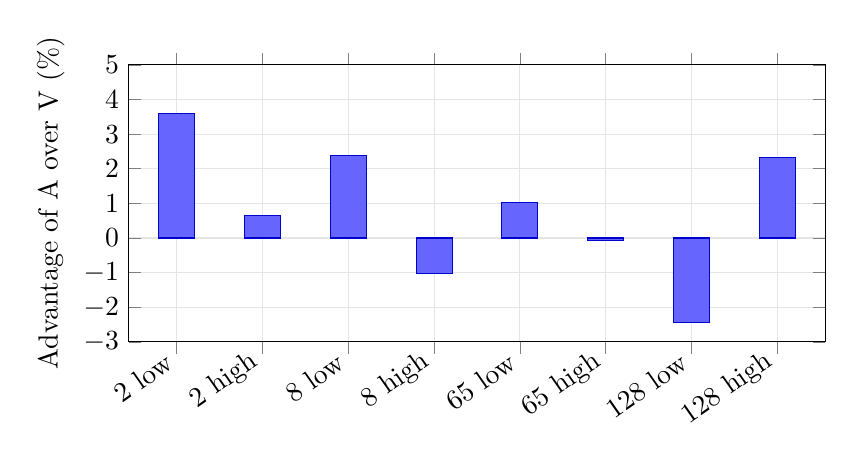
\begin{tikzpicture}
\begin{axis}[
 width=.86\linewidth,height=5.1cm,
 ybar,bar width=13pt,enlarge x limits=.08,
 ymin=-3,ymax=5,ytick={-3,-2,-1,0,1,2,3,4,5},
 xtick={1,2,3,4,5,6,7,8},
 xticklabels={2 low,2 high,8 low,8 high,65 low,65 high,128 low,128 high},
 x tick label style={rotate=35,anchor=east},
 ylabel={Advantage of A over V (\%)},
 grid=major,grid style={gray!20},
]
\addplot+[fill=blue!60,draw=blue!80!black,mark=none] coordinates
 {(1,3.583) (2,.647) (3,2.385) (4,-1.020)
  (5,1.032) (6,-.061) (7,-2.443) (8,2.320)};
\end{axis}
\end{tikzpicture}}
\caption{Relative difference in complete-episode medians at $H=1\,024$: $100(\mathrm{V}-\mathrm{A})/\mathrm{V}$. Positive bars favor annotation. Differences remain small under Étendue3D load; the high-grade 65D bar is almost zero. This earlier B1 graph does not measure B1W~\cite{b1horizons}.}
\label{fig:b1horizons}
\end{figure}
\FloatBarrier

At $H=1\,024$ , the greatest descriptive gain of the annotation is 3.6 \% in 2D low grade. Two retreats exceed 1 \% and a third unfavourable difference of 0.06 \% is almost equal: the annotated median is greater in three of the eight cells. The routes have exactly the same allocations in each cell. The difference in LLVM code in the loop therefore does not become a uniform episode gain when copies, validations, readings and independently owned outputs are repeated. Interference and close deviations prohibit a production choice based on these only medians~\cite{b1horizons} .

\paragraph{B1W: validated workspaces for repeated products.}
\emph{Why test it?} At $H=1\,024$, the earlier B1 paths allocate 39\,096--39\,184 objects and 3.38--4.28 million bytes per episode. Most of this cost is repeated plan validation and buffer construction. B1W tests whether retaining a validated plan and private buffers can amortize that cost while reading changing coefficients at every call and returning $H$ distinct, independently owned sparse outputs. The outputs themselves must still be allocated.

\emph{Implementation and correctness.} The first constructor authenticates a supplied plan against a newly computed canonical plan, then retains the canonical snapshot and private buffers. Later mutations of the supplied plan cannot change the snapshot. The second constructor builds the canonical plan directly from the two operands, without first constructing and authenticating an external plan. Both check the algebra, support, and numeric type at each call, reread the coefficients, and reject changes to the metric, basis, support, or dense size before accumulation. Neither changes the public Garamon.jl kernel. The external-plan constructor passes 847/847 targeted tests with forced bounds and again with normal bounds; the direct constructor passes 1\,018/1\,018 under each setting. GaramonBench functional checks pass 64/64 and 873/873 for the first constructor, and 64/64 and 1\,161/1\,161 for the second; its full suite passes 1\,038/1\,038 after the direct constructor is added~\cite{b1wpreflight,b1wdirect}.

\emph{Experiment and results.} The first PerfChecker preflight qualifies 144/144 cases and 3\,024 observations. It compares checked B1, annotated B1, and external-plan B1W for $n=2,8,65,128$, low- and high-grade supports, and $H=1,32,1\,024$, in two orders. The full episode includes plan construction, authentication, private-buffer creation, and all owned outputs. External-plan B1W loses all eight cells at $H=1$ and all eight at $H=32$, but beats the faster B1 median in seven of eight cells at $H=1\,024$ by roughly 1.3--2.0 times. The exception is low-grade 65D, about 8\% slower than checked B1 in that batch. Its long-episode allocations fall to 0.99--1.35 million bytes and 8\,700--10\,000 objects, compared with 3.38--4.28 million bytes and about 39\,000 objects for B1~\cite{b1wpreflight}.

A second paired preflight compares four routes, including direct-construction B1W, in 192/192 qualified cases and 4\,032 observations. It uses Julia 1.13, \code{--check-bounds=auto}, \code{-O2}, native CPU, one thread, a positive metric, two orderings, and seven samples in each of the build, warm, and complete-episode phases. The independent oracle and ownership checks cover every output before and after measurement. Table~\ref{tab:b1wdirect} gives the complete-episode medians at $H=1\,024$ from this \emph{single} batch. ``Best B1'' is the lower of the checked and annotated medians in that cell, a descriptive comparator rather than a trained selector. Direct B1W wins all eight cells against it, by 1.28--2.44 times. Against external-plan B1W, direct construction is faster in five cells, nearly tied in one, and slower in two; the timing difference is not uniform~\cite{b1wdirect}.

\begin{table}[ht]
\centering\footnotesize
\begin{tabular}{@{}rlrrrr@{}}
\toprule
$n$ & Support & Best B1 & External B1W & Direct B1W & B1/direct \\
\midrule
2 & low  & 635.130 & 313.817 & 301.672 & 2.11 \\
2 & high & 629.296 & 316.411 & 314.627 & 2.00 \\
8 & low  & 664.858 & 324.073 & 320.281 & 2.08 \\
8 & high & 785.484 & 441.616 & 321.831 & 2.44 \\
65 & low  & 915.324 & 598.815 & 599.103 & 1.53 \\
65 & high & 1\,082.801 & 813.296 & 845.606 & 1.28 \\
128 & low & 1\,305.717 & 949.929 & 1\,018.365 & 1.28 \\
128 & high & 1\,481.648 & 1\,092.356 & 1\,026.341 & 1.44 \\
\bottomrule
\end{tabular}
\caption{Complete-episode medians in microseconds at $H=1\,024$, including construction and independent owned outputs. Four paired routes, two orders, 14 observations per route and cell. Ratios above one favor direct B1W; all figures come from the second preflight under concurrent Étendue3D activity~\cite{b1wdirect}.}
\label{tab:b1wdirect}
\end{table}

\begin{figure}[ht]
\centering
\IfFileExists{exploratory_b1wdirect.pdf}{\includegraphics[width=.92\linewidth]{exploratory_b1wdirect.pdf}}{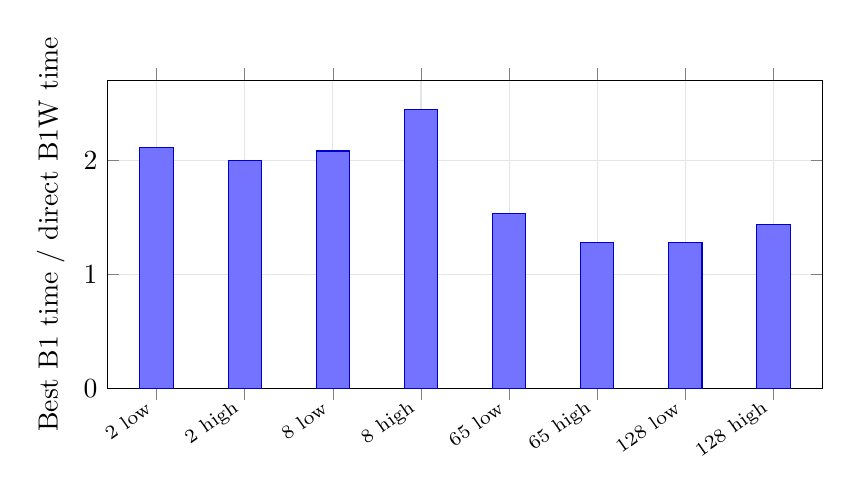
\begin{tikzpicture}
\begin{axis}[
 width=.88\linewidth,height=5.5cm,
 ybar,bar width=12pt,enlarge x limits=.08,
 ymin=0,ymax=2.7,ytick={0,1,2},
 xtick={1,2,3,4,5,6,7,8},
 xticklabels={2 low,2 high,8 low,8 high,65 low,65 high,128 low,128 high},
 xticklabel style={rotate=35,anchor=east,font=\scriptsize},
 ylabel={Best B1 time / direct B1W time},
 grid=major,grid style={gray!20},
]
\addplot+[fill=blue!55,draw=blue!80!black] coordinates
 {(1,2.11) (2,2.00) (3,2.08) (4,2.44) (5,1.53) (6,1.28) (7,1.28) (8,1.44)};
\end{axis}
\end{tikzpicture}}
\caption{Direct B1W speedup over the faster checked or annotated B1 episode at $H=1\,024$. Each bar is paired within the second preflight and includes construction and owned outputs; it is not an isolated-machine speedup estimate~\cite{b1wdirect}.}
\label{fig:b1wdirect}
\end{figure}
\FloatBarrier

The cold construction cost dominates shorter episodes: direct B1W loses all eight cells at $H=1$ and all eight at $H=32$. Across the eight fixtures, the median build phase alone spans 37.075--524.196~\(\mu\)s for direct B1W versus 5.412--13.230~\(\mu\)s for the B1 paths. At $H=1\,024$, direct B1W allocates 0.98--1.32 million bytes in 8\,535--9\,765 allocations, versus 3.38--4.28 million bytes in 39\,098--39\,186 allocations for B1; all $H$ output dictionaries remain distinct. The retained workspace memory is admitted under a separate budget, and concurrent sharing or mutation of the workspace is outside this contract. Both preflights ran under declared concurrent Étendue3D load. Mixed or degenerate metrics, denser and central-grade supports, memory ceilings, isolated reruns, and an equivalent C++ workspace remain untested. These observations do not establish an automatic reuse threshold~\cite{b1wpreflight,b1wdirect}.

\paragraph{B1W single-pass sparse output: why test it?}
The direct B1W workspace still built a dictionary of nonzero coefficients and passed it to the public \code{SparseMultiVector} constructor, which validated and copied that dictionary. In a qualified 8D profile of an episode with 1\,024 independently owned outputs, stacks containing this constructor accounted for 409\,600 of 886\,144 profiled allocation bytes; these inclusive stack counts overlap other categories. A narrower experiment can therefore ask whether filling each \emph{new} output dictionary once reduces allocations without changing any product, support check, path order, or ownership guarantee. The experimental route creates an empty sparse multivector through its public constructor and inserts only final nonzero coefficients into its fresh dictionary. It remains under \code{perf/}, outside the public Garamon.jl API. Its proof relies on unique, already checked canonical output masks and on exclusive ownership of the private workspace~\cite{b1wsinglepass}.

\emph{Validation and paired experiment.} The targeted suite passes 1\,066/1\,066 assertions with forced bounds and again with normal bounds, including mixed and degenerate metrics, \code{Int64} and \code{Float64}, coefficient changes, and independently owned outputs. At this first single-pass preflight, the complete GaramonBench suite passes 1\,051/1\,051 assertions, with 1\,513/1\,513 targeted runtime assertions. PerfChecker qualifies 96/96 paired cases and 2\,016 observations across $n=2,8,65,128$, low- and high-grade supports, $H=1,32,1\,024$, two routes, and two orders. Each phase has seven samples. Julia 1.13.0 ran with automatic bounds checks, \code{-O2}, native target, one thread, and a positive metric. Complete episodes include construction and retain $H$ distinct outputs; an independent oracle checks them before and after timing. These timing measurements still share the machine with Étendue3D~\cite{b1wsinglepass}.

\begin{table}[ht]
\centering\footnotesize
\begin{tabular}{@{}rlrrrr@{}}
\toprule
$n$ & Support & Earlier B1W & Single pass & Earlier/new & Allocation bytes, earlier $\rightarrow$ new \\
\midrule
2 & low  & 347.648 & 270.212 & 1.29 & 984\,392 $\rightarrow$ 673\,096 \\
2 & high & 320.791 & 283.412 & 1.13 & 984\,392 $\rightarrow$ 673\,096 \\
8 & low  & 388.874 & 306.918 & 1.27 & 986\,360 $\rightarrow$ 675\,064 \\
8 & high & 362.924 & 331.396 & 1.10 & 987\,512 $\rightarrow$ 676\,216--678\,304 \\
65 & low  & 645.242 & 626.746 & 1.03 & 1\,272\,400 $\rightarrow$ 834\,168 \\
65 & high & 726.926 & 629.718 & 1.15 & 1\,291\,216--1\,295\,352 $\rightarrow$ 848\,848 \\
128 & low & 845.126 & 762.913 & 1.11 & 1\,297\,320 $\rightarrow$ 871\,376 \\
128 & high & 860.478 & 837.508 & 1.03 & 1\,316\,136 $\rightarrow$ 873\,768 \\
\bottomrule
\end{tabular}
\caption{B1W complete-episode medians in microseconds at $H=1\,024$, pooled over two orders in the single-pass preflight. Ratios above one favor single-pass output. Allocation bytes are per episode; two cells span slightly different values between orders. These are paired observations under concurrent load, not isolated speed estimates~\cite{b1wsinglepass}.}
\label{tab:b1wsinglepass}
\end{table}

\begin{figure}[ht]
\centering
\IfFileExists{exploratory_b1wsinglepass.pdf}{\includegraphics[width=.92\linewidth]{exploratory_b1wsinglepass.pdf}}{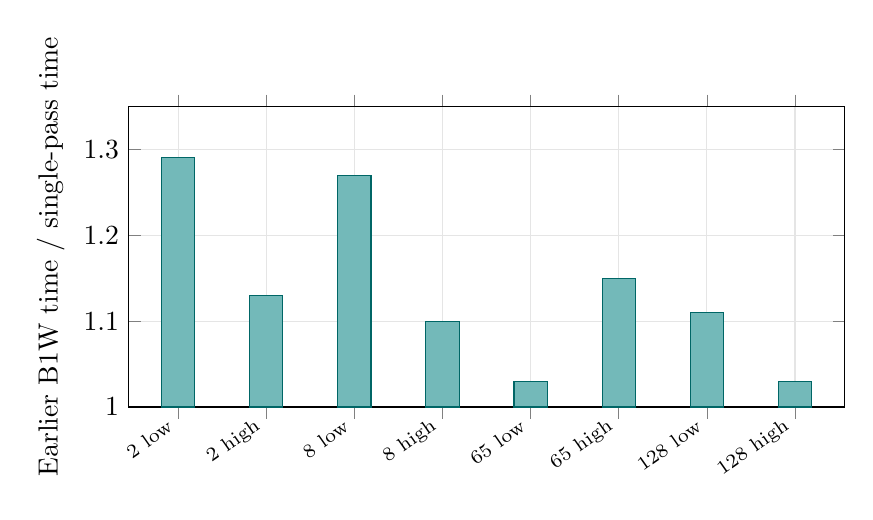
\begin{tikzpicture}
\begin{axis}[
 width=.88\linewidth,height=5.4cm,
 ybar,bar width=12pt,enlarge x limits=.08,
 ymin=1,ymax=1.35,ytick={1,1.1,1.2,1.3},
 xtick={1,2,3,4,5,6,7,8},
 xticklabels={2 low,2 high,8 low,8 high,65 low,65 high,128 low,128 high},
 xticklabel style={rotate=35,anchor=east,font=\scriptsize},
 ylabel={Earlier B1W time / single-pass time},
 grid=major,grid style={gray!20},
]
\addplot+[fill=teal!55,draw=teal!80!black] coordinates
 {(1,1.29) (2,1.13) (3,1.27) (4,1.10) (5,1.03) (6,1.15) (7,1.11) (8,1.03)};
\end{axis}
\end{tikzpicture}}
\caption{Pooled long-episode medians favor the single-pass sparse-output route in all eight tested fixtures. The first-order 8D high-grade median reverses this ranking (ratio 0.977), so the pooled bars should be read with the paired results and the concurrent-load limitation~\cite{b1wsinglepass}.}
\label{fig:b1wsinglepass}
\end{figure}
\FloatBarrier

At $H=1\,024$, the pooled median is lower in eight of eight fixtures, by factors of 1.03--1.29; 15 of 16 individual-order medians agree. Allocation counts fall by about 2\,046--2\,048 per episode, and bytes by about 31--35\% in this corpus. At $H=1$, the new route wins six of eight pooled cells (ten of sixteen individual orders); at $H=32$, six of eight (twelve of sixteen). Construction can dominate these shorter episodes. Separate PerfChecker profiles of the 8D long episode qualify CPU, allocations, latency, GC, memory, and typing on both routes. Stacks containing \code{SparseMultiVector} fall from 409\,600 to 81\,920 profiled allocation bytes, while total profiled bytes fall from 886\,144 to 625\,904; overlapping stacks cannot be added. A mask-type union remains in the construction wrapper. The profiles support the allocation explanation but do not supply a second paired timing verdict. A hardware-monitored rerun, broader metrics and supports, and a matching public-route and C++ contract are still needed before selecting this route automatically~\cite{b1wsinglepass}.

\emph{Twelve-dimension extension.} A separate $H=1\,024$ screen repeats this Julia-to-Julia comparison at $n=2,3,4,6,8,12,16,32,64,65,96,128$, with two four-term support families, a positive diagonal metric, two route orders, and independently owned sparse outputs. Julia 1.13.0 uses automatic bounds checks, \code{-O2}, native target, and one thread. PerfChecker qualifies 96/96 cases and 2\,016 observations; the independent \code{Int64} oracle checks outputs before and after measurement. Allocation bytes fall by 30.1--34.8\% in all 24 dimension/support cells. All 24 pooled medians numerically favor single-pass output, but the 32D high-grade ratio is only 1.000025; only 46 of 48 order-specific medians favor it. The exceptions are 32D high grade in the second order (ratio 0.978) and 64D high grade in the second order (0.945). The low-grade masks remain $0,1,2,3$ and span only two active directions; high-grade supports also contain just four terms. Neither dense nor full central-grade support is tested. Étendue3D still shares the machine, so this screen confirms the allocation reduction for its sparse corpus without establishing stable timing or a routing threshold. After adding the twelve-dimension plan, the complete GaramonBench suite passes 1\,054/1\,054 assertions~\cite{b1wsinglepass12d}.


\emph{Separate replay without other declared user computation.} A second archive repeats the same twelve dimensions, four-term support families, positive metric, $H=1\,024$, and reversed route orders. It independently qualifies 96/96 cases and 2\,016 observations, with owned outputs checked against the integer oracle. The median of 48 within-pair earlier/single-pass ratios is 1.106, and the single-pass route has the lower complete-episode median in 48/48 pairs; allocation bytes fall by 30.2--34.7\% in those pairs. The concurrent Étendue3D screen had 46/48 order-specific wins and a median paired ratio of 1.113. These are \emph{separate} campaigns and are not pooled. The replay's operator label \code{isolated} and empty competing-workload label record that no other user computation was declared; they do not reserve a CPU core or stop desktop services. The improvement is descriptive for long episodes with four terms per operand, not a threshold for dense, central-grade, or other-metric products~\cite{b1wsinglepass12d}.

The C++ move patch has its \emph{own} upstream baseline with identical inputs and the same \code{Mvec} representation. Its allocation counts are deterministic for Euclidean EGA3/EGA7 with \code{Float64}; timings remain exploratory under the same concurrent load. The allocation result does not establish a gain for other algebras, scalar types, or compilers.

\Needspace{10\baselineskip}
\subsection{Order of the next validations}
The experimental program has four stages:
\begin{enumerate}
\item \textbf{Preflight and technique validation.} Define each technique's output contract, eligible workloads, budgets, and baselines. Check correctness against an independent oracle, expected rejection cases, and reproducibility of identities under Julia 1.13. This remains active for prototypes with incomplete coverage.
\item \textbf{Broader PerfChecker scans and optimization.} Cross ambient dimensions with scalar, multiple-output, and complete products; include degenerate and nonorthogonal metrics, support patterns, densities, reuse horizons, numeric types, threads, and processes. Keep complete episodes, preparation, raw samples, medians and tails, allocations, GC time, code size, peak RSS, first compilation, and budget refusals. Profile the actual cost before each optimization and measure again afterward. For B1W, isolate canonical construction, the remaining mask-type union, and output materialization; repeat both constructors and the single-pass variant against B1 on an idle machine with identical owned outputs.
\item \textbf{Matched C++/Julia comparison.} After each route is validated and optimized, compare kernels with the same algorithm, supports, coefficients, outputs, precision rules, and preparation costs. Record compilation and cold-start costs separately. The packed comparison above remains an exploratory pilot.
\item \textbf{Classification by workload, including dimension.} Derive a selector only from stable, repeated crossovers. An unstable or close crossover requires more evidence; one case cannot define a universal dimension boundary.
\end{enumerate}

The accompanying campaign archives contain the sources, corpus, fingerprints, and exclusions. Generation and long-trace campaigns are documented under \code{perf/} in the Julia repository. Three accompanying CSV files document I15.6. Tables here select representative rows; native CSV files remain authoritative for coverage. Julia 1.13.0 is the validation environment. The earlier single-thread full suite passed 6\,031/6\,031 assertions, including 402 for the exact selector~\cite{fullsuites}; after grouped batch validation the Garamon.jl suite passes 6\,034/6\,034 under each bounds policy~\cite{packonce}. After the twelve-dimension B1W plan is added, the GaramonBench suite passes 1\,054/1\,054 assertions~\cite{b1wsinglepass12d}. These counts establish correctness only on the tested families. The B1W replay, matched Julia/C++ replays, packed GPU pilot, pinned-output screens, CPU4/GPU comparison, resident-sum screen, fusion screen, focused replay, and graph pilot have distinct qualification archives; their operator-declared lack of competing user work does not certify hardware isolation, particularly while the GPU drives the display. The resident-sum and fusion broad screens each record 648 qualified cases and 13\,608 observations; the fusion replay separately records 54 cases and 1\,134 observations; the graph pilot qualifies 192 cases and 4\,032 observations after excluding its incomplete first attempt~\cite{residentsum,residentfusion,residentgraph}. The high-dimensional baseline and grouped-validation replay each retain 320 cases and 6\,720 observations in separate ten-process archives~\cite{residenthighdim,packonce}. External reproduction also requires a frozen copy of the private Julia worktree. No general native precompilation catalog, automatic GPU threshold, or tuned selector is claimed. Approximate pruning remains outside the exact-product API.

\subsection{Toward a benchmark shared across machines and teams}
The separate \code{GaramonBench.jl} package distributes an initial Julia/C++ benchmark with configurations, C++ sources, and campaign manifests~\cite{garamonbench}. DrWatson.jl~\cite{drwatson} expands parameter grids, names cases, and records Git provenance. The initial package passed 25 tests. Its Julia campaign qualified 8/8 PerfChecker cases with 56 warm samples; its C++/Julia driver qualified 4/4 cases with 124 warm samples and 305 native observations. Both smoke tests ran during Étendue3D activity. Their timed scopes differ, so times are not compared across campaigns. The C++ driver uses sources shipped in the package; upstream \code{Mvec} remains a descriptive, unmatched route.

The orchestrator subsequently gained thirteen executable recipes. Its 47 introduction checks passed, followed by a complete suite of 1\,030/1\,030 assertions at that stage, including 802 for the B1 driver~\cite{garamonrecipes,fullsuites}. The newer \code{long-horizon} command ran one recipe and qualified 2/2 cases with four samples under Étendue3D interference; the other twelve recipes were integrated but not requalified by that command. This smoke test supports no speed ranking, and an isolated full run remains open. Shared manifests help laboratories exchange equivalent cases without treating times on unlike processors as interchangeable. Later B1W additions raised the full suite to 1\,054/1\,054 assertions, as reported above~\cite{b1wsinglepass12d}.

\begin{figure}[ht]
\centering
\IfFileExists{ega3_vector_libraries.pdf}{%
  \includegraphics[width=.9\linewidth]{ega3_vector_libraries.pdf}%
}{%
  \fbox{\parbox[c][45mm][c]{.86\linewidth}{\centering Awaiting validated EGA3 vector measurements from the dedicated benchmark machine.}}%
}
\caption{EGA3 vector products across Garamon.jl, GAL, and Versor. The plot is replaced as validated cases become available. These libraries use different internal strategies, so the comparison describes whole-library behavior rather than a language effect.}
\label{fig:external-ga-vectors}
\end{figure}

\begin{figure}[ht]
\centering
\IfFileExists{exploratory_benchvariabilite.pdf}{\includegraphics[width=.92\linewidth]{exploratory_benchvariabilite.pdf}}{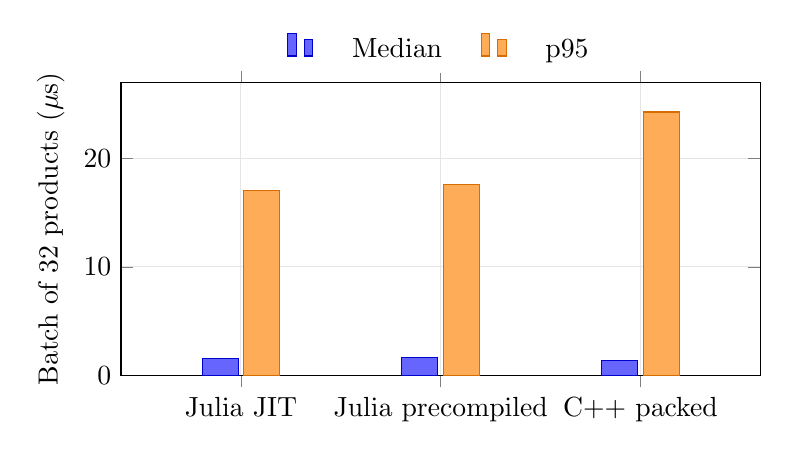
\begin{tikzpicture}
\begin{axis}[
 width=.8\linewidth,height=5.3cm,
 ybar,bar width=13pt,enlarge x limits=.3,
 ymin=0,ymax=27,
 xtick={1,2,3},
 xticklabels={Julia JIT,Julia precompiled,C++ packed},
 ylabel={Batch of 32 products (\(\mu\)s)},
 grid=major,grid style={gray!20},
 legend style={at={(.5,1.03)},anchor=south,legend columns=2,column sep=12pt,draw=none,fill=white},
]
\addplot+[fill=blue!60,draw=blue!80!black,mark=none] coordinates
 {(1,1.554) (2,1.604) (3,1.338)};
\addplot+[fill=orange!65,draw=orange!85!black,mark=none] coordinates
 {(1,17.026) (2,17.587) (3,24.284)};
\legend{Median,p95}
\end{axis}
\end{tikzpicture}}
\caption{New \code{GaramonBench.jl} campaign on EGA3 mixed support, 32 products per batch: three \emph{matched} routes with 31 samples each. The long timing tail under concurrent load makes fine median comparisons premature. Upstream C++ \code{Mvec} and older campaigns are excluded because their output contracts or measurement footprints differ.}
\label{fig:benchvariabilite}
\end{figure}

Each replicated observation should record exact inputs and outputs, metric, numeric type, executed strategy, generator and kernel fingerprints, Julia and C++ versions, compiler version, machine, thread count, cache state, and degree of machine isolation. A manifest should reconstruct the same arithmetic task on different machines. Timing analysis should keep machines and cold versus warm states separate. An isolated full rerun can test the stability of current findings; a second site can test their transfer without pooling raw microseconds from unlike processors. Language comparisons should use the same strategy, supports, coefficients, outputs, precision, and timed preparation. Raw data, budget rejections, and reproduction commands should accompany published results.

\FloatBarrier
\Needspace{28\baselineskip}
\section{Conclusion}
The code audit shows that Garamon C++ organizes computation around dense grade storage and recursive prefix traversal. Garamon.jl can instead adapt work to operand supports and requested outputs without generating a separate library. In the measured families, a complete product remains appropriate for some small cases, a targeted join wins in others, and workspaces repay preparation during repeated use by reducing warm allocations. Grade blocks, caches, and factorized forms require structure and reuse sufficient to pay for their construction or conversion; the observed negative cases rule out one uniform strategy. In a paired 65D kernel, \code{UInt128} avoids much of the cost of arbitrary-width masks.

The N01 binary-ranking prototype often beats a prepared plan on short episodes but loses every configuration in its grid at $H=1\,024$; the timing remains a screen under concurrent load. The separate B4 compact-rank bounds-check pilot confirms local elimination of a checked LLVM path under \code{auto} and small descriptive long-episode gains in two 12D campaigns, but neither an allocation reduction nor a stable routing threshold. N05 avoids a full multivector expansion for a vector-chain scalar, but its \code{Float64} cancellation counterexample and the lack of a general scalar-only baseline prevent automatic routing. K3 reuses contractions and improves a stable 65D fixture and some amortized screening episodes, but loses small requests; 176 validated identities establish no threshold. N04 certifies $A^2=\lambda1$ on its tested cases: reuse wins for two stable fixtures, while binary powering wins for the changing or rejected input. N03 validates radical inversion across 1\,512 screening cases in two orders without a reproducible timing threshold. It still needs isolated reruns, the 18\,000-identity manifest, near-singular quotients, and the cost of a general metric.

A targeted native catalog makes the first known EGA3 prepared product fast after restart, whereas newly generated topologies still recompile in this protocol. Approximate pruning can save time at the cost of error; restoring the exact trajectory was slower in the initial median comparison. \code{TripleJoinPlan} wins all twenty measured cells at 1\,024 calls with preparation included and loses all twenty at one call. Those results use modest supports and concurrent machine load. The first exact strategy selector runs and passes its paired smoke test, but new families, long horizons, and isolated repeats must qualify its decisions. A matched four-thread packed CPU pilot wins 66/72 complete episodes over sequential CPU at $H=8\,192$; other thread counts and process gains remain untested. The GPU beats sequential CPU in 57/72 episodes at that horizon but beats CPU4 in only 13/72, showing that the CPU baseline changes the crossover. A CUPTI diagnosis finds host-output copies longer than kernels in two fixtures. Pinned host output wins every pair in a small long-horizon pilot but only 30/72 in a twelve-dimension screen. Under a separate exact resident-sum contract, the GPU wins 72/72 complete episodes against CPU4 at $H=1\,024,R=32$ but only 1/72 at $H=32,R=32$; four reused input sets and a single final host output explain why this cannot replace the per-product-output comparison. None of these GPU results establishes an automatic threshold. The matched packed C++ kernel is exact in 64 cases; two fresh, order-balanced 64-case replays find Julia faster in 4/8 long-horizon pairs, with median Julia/C++ ratio 1.032. These results and the separate upstream \code{Mvec} timings establish no general language winner.

Within that \emph{same resident-sum output contract}, one fused GPU kernel wins 72/72, 63/72, and 71/72 complete episodes against the prior $R$-kernel GPU at $(H,R)=(32,32),(1\,024,8),(1\,024,32)$. It still loses most $H=32,R=32$ single-output episodes to CPU4 (22/72 wins). One 12D higher-rank reversal at $H=1\,024,R=32$ remains in the broad archive although six focused replays favor fusion; its cause is unknown. A separate CUDA Graph pilot with $Q$ repeated owned outputs wins almost all comparisons against ordinary $R$-kernel GPU but none against fusion. In that new campaign, fusion wins 16/16 paired CPU4 episodes at $(H,R,Q)=(32,32,32)$; the different single-output campaign cannot isolate $Q$ as the cause. Session length must enter future selection studies. Fusion and graphs remain experimental, with no automatic threshold or matched C++ comparison.

The high-dimensional resident screen strengthens the fixed-support comparison within Julia: fusion beats CPU4 and the graph in all 40 paired episodes at each of two workloads from 129D through 8\,192D. A later CPU profile identifies repeated metric and basis validation during packing; a separate exact rerun with grouped validation reduces the 8\,192D fused build from 34.43 to 2.28~ms and its complete episode from 45.84 to 12.50~ms. The before/after times come from different fresh-process campaigns, while route comparisons within each campaign are paired. The metric remains a compact \code{Diagonal}; neither its storage nor the 6~GiB process budget defines a universal dimensional ceiling. Denser supports, other signatures, changing values, peak VRAM, packing copies, and a matched C++ route remain open~\cite{residenthighdim,packonce}.

The B1 bounds-checking pilot qualifies 96 cases across its two dimension scans and finds no uniform complete-episode gain. Its horizon preflight qualifies 96 further cases at $H=1,32,1\,024$; annotation improves the long-horizon median by at most 3.6\% in these fixtures, with identical allocations. Two subsequent B1W workspace constructors validate independent owned outputs and reduce repeated allocations. The external-plan version wins seven of eight long-horizon cells in its first preflight; the direct version wins eight of eight against the faster B1 route in its own paired preflight, by 1.28--2.44 times. Both lose all eight cells at $H=1$ and $H=32$, and direct versus external construction is not uniformly faster. A later single-pass output variant avoids a dictionary copy. In a concurrent twelve-dimension screen with four-term supports, it cuts allocation bytes by 30.1--34.8\% and wins 46/48 order-specific long-episode pairs. A separate replay without other declared user computation cuts bytes by 30.2--34.7\% and wins 48/48, with median paired ratio 1.106. The replay does not certify hardware isolation, and these sparse positive-metric cases do not establish a routing threshold. Separately, moving four temporary \code{Kvec} objects in upstream C++ halves Eigen-buffer allocations in 32 paired groups with 67\,840 exact products checked; an isolated timing study remains. The next step is to validate, profile, and optimize each route independently, then repeat matched C++/Julia comparisons before classifying workloads. Controlled timing reruns are needed before broader speed claims.

\begin{thebibliography}{99}
\small
\bibitem{breuils2019} S. Breuils, V. Nozick and L. Fuchs, ``Garamon: A Geometric Algebra Library Generator'', \emph{Advances in Applied Clifford Algebras} 29, 69 (2019). \url{https://doi.org/10.1007/s00006-019-0987-7}.
\bibitem{breuils2020} S. Breuils, V. Nozick and A. Sugimoto, ``Computational Aspects of Geometric Algebra Products of Two Homogeneous Multivectors'' (2020). \url{https://arxiv.org/abs/2002.11313}.
\bibitem{garamoncpp} Garamon C++ repository, \href{https://github.com/vincentnozick/garamon/tree/6267161e35be57873fa553f266ef04f2ba32d2e5}{commit 6267161}.
\bibitem{cppmain} Garamon C++, \code{src/main.cpp}, generation pipeline, \href{https://github.com/vincentnozick/garamon/blob/6267161e35be57873fa553f266ef04f2ba32d2e5/src/main.cpp}{commit 6267161}.
\bibitem{cppindex} Garamon C++, \code{src/ProductTools.cpp}, blade indexing, \href{https://github.com/vincentnozick/garamon/blob/6267161e35be57873fa553f266ef04f2ba32d2e5/src/ProductTools.cpp}{commit 6267161}.
\bibitem{cppdispatch} Garamon C++, \code{src/ProductToString.cpp}, product emission and dispatch, \href{https://github.com/vincentnozick/garamon/blob/6267161e35be57873fa553f266ef04f2ba32d2e5/src/ProductToString.cpp}{commit 6267161}.
\bibitem{cppmvec} Garamon C++, \code{data/Mvec.hpp}, stockage and dispatch, \href{https://github.com/vincentnozick/garamon/blob/6267161e35be57873fa553f266ef04f2ba32d2e5/data/Mvec.hpp}{commit 6267161}.
\bibitem{cppgeometric} Garamon C++, \code{data/Geometric.hpp}, recursive product, \href{https://github.com/vincentnozick/garamon/blob/6267161e35be57873fa553f266ef04f2ba32d2e5/data/Geometric.hpp}{commit 6267161}.
\bibitem{cppmetric} Garamon C++, \code{src/MetricTools.cpp}, grade-wise basis transformations, \href{https://github.com/vincentnozick/garamon/blob/6267161e35be57873fa553f266ef04f2ba32d2e5/src/MetricTools.cpp}{commit 6267161}.
\bibitem{leapfrog} T. L. Veldhuizen, ``Leapfrog Triejoin: a Worst-Case Optimal Join Algorithm'' (2012). \url{https://arxiv.org/abs/1210.0481}.
\bibitem{sparseworkspace} G. Zhang, O. Hsu and F. Kjolstad, ``Compilation of Modular and General Sparse Workspaces'', \emph{Proceedings of the ACM on Programming Languages} 8 (PLDI), article 196 (2024). \url{https://doi.org/10.1145/3656426}.
\bibitem{taco} F. Kjolstad, S. Kamil, S. Chou, D. Lugato and S. Amarasinghe, ``The Tensor Algebra Compiler'', \emph{Proceedings of the ACM on Programming Languages} 1 (OOPSLA), article 77 (2017). \url{https://doi.org/10.1145/3133901}.
\bibitem{finch} W. Ahrens, T. Fields Collin, R. Patel, K. Deeds, C. Hong and S. Amarasinghe, ``Finch: Sparse and Structured Tensor Programming with Control Flow'' (2024). \url{https://arxiv.org/abs/2404.16730}.
\bibitem{galley} K. Deeds, W. Ahrens, M. Balazinska and D. Suciu, ``Galley: Modern Query Optimization for Sparse Tensor Programs'', preprint (2024). \url{https://arxiv.org/abs/2408.14706}.
\bibitem{gaalop} C. Schwinn, D. Hildenbrand, F. Stock and A. Koch, ``Gaalop 2.0 --- a geometric algebra algorithm compiler'', \emph{GraVisMa} (2010). \url{https://publica.fraunhofer.de/entities/publication/25f7307c-0502-402d-b63a-6f855b9226d8}.
\bibitem{oseledets} I. V. Oseledets, ``Tensor-Train Decomposition'', \emph{SIAM Journal on Scientific Computing} 33(5), 2295--2317 (2011). \url{https://doi.org/10.1137/090752286}.
\bibitem{minato} S. Minato, ``Zero-Suppressed BDDs for Set Manipulation in Combinatorial Problems'', \emph{DAC}, 272--277 (1993). \url{https://doi.org/10.1145/157485.164890}.
\bibitem{tinylfu} G. Einziger, R. Friedman and B. Manes, ``TinyLFU: A Highly Efficient Cache Admission Policy'' (2015). \url{https://arxiv.org/abs/1512.00727}.
\bibitem{sieve} Y. Zhang, J. Yang, Y. Yue, Y. Vigfusson and K. V. Rashmi, ``SIEVE is Simpler than LRU: an Efficient Turn-Key Eviction Algorithm for Web Caches'', \emph{NSDI}, 1229--1246 (2024). \url{https://www.usenix.org/conference/nsdi24/presentation/zhang-yazhuo}.
\bibitem{satzilla} L. Xu, F. Hutter, H. Hoos and K. Leyton-Brown, ``SATzilla: Portfolio-Based Algorithm Selection for SAT'', \emph{Journal of Artificial Intelligence Research} 32, 565--606 (2008). \url{https://doi.org/10.1613/JAIR.2490}.
\bibitem{aslib} B. Bischl and al., ``ASlib: A Benchmark Library for Algorithm Selection'' (2015). \url{https://arxiv.org/abs/1506.02465}.
\bibitem{autofolio} M. Lindauer, F. Hutter, H. Hoos and T. Schaub, ``AutoFolio: An Automatically Configured Algorithm Selector'', \emph{IJCAI} (2017). \url{https://doi.org/10.24963/ijcai.2017/715}.
\bibitem{egg} M. Willsey and al., ``egg: Fast and Extensible Equality Saturation'' (2020). \url{https://arxiv.org/abs/2004.03082}.
\bibitem{fftw} M. Frigo and S. G. Johnson, ``The Design and Implementation of FFTW3'', \emph{Proceedings of the IEEE} 93(2), 216--231 (2005). \url{https://www.fftw.org/fftw-paper-ieee.pdf}.
\bibitem{juliaprecompile} Julia, manual ``Module initialization and precompilation''. \url{https://docs.julialang.org/en/v1/manual/modules/#Module-initialization-and-precompilation}.
\bibitem{juliathreads} Julia, manual ``Multi-Threading''. \url{https://docs.julialang.org/en/v1/manual/multi-threading/}.
\bibitem{cudaperf} CUDA.jl, ``Performance Tips''. \url{https://cuda.juliagpu.org/dev/tutorials/performance/}.
\bibitem{shap} S. M. Lundberg and S.-I. Lee, ``A Unified Approach to Interpreting Model Predictions'' (2017). \url{https://arxiv.org/abs/1705.07874}.
\bibitem{rhee} C.-H. Rhee and P. W. Glynn, ``Unbiased Estimation with Square Root Convergence for SDE Models'' (2015). \url{https://web.stanford.edu/~glynn/papers/2015/RheeG15.html}.
\bibitem{drwatson} G. Datseris, J. Isensee, S. Pech and T. Gál, ``DrWatson: the perfect sidekick for your scientific inquiries'', \emph{Journal of Open Source Software} 5(54), 2673 (2020). \url{https://doi.org/10.21105/joss.02673}.
\bibitem{garamonbench} ``GaramonBench.jl: reproducible Julia/C++ package'', \url{https://github.com/Mirage-Interactive-Fr/GaramonBench.jl}, with archived campaign data (September 2026).
\bibitem{garamonrecipes} ``GaramonBench: orchestration of benchmark recipes'', archived campaign data and \code{long-horizon} smoke-test archive, supplied with this article (September 27, 2026).
\bibitem{fullsuites} ``Validation of the complete Garamon.jl and GaramonBench.jl suites'', archived campaign data, supplied with this article (September 27, 2026).
\bibitem{n01report} ``N01: binary-rank reduction of supports'', archived campaign data, summary and episode samples \path{n01-binary-rank-episodes/}, supplied with this article (September 27, 2026).
\bibitem{k1decision} ``K1: comparison of four routes and first K1v2 batch'', archived campaign data, supplied with this article (September 27, 2026).
\bibitem{k1audit} ``K1v2: replay coverage audit'', local file \path{k1-decision-coverage.toml}, supplied with this article (September 27, 2026).
\bibitem{b4bounds} ``B4: compact binary-rank bounds-checking preflight'', archived campaign data, with links to the 8D smoke test, two 12D campaigns, and targeted order-reversal reruns, supplied with this article (September 27, 2026).
\bibitem{n03report} ``N03: inversion through a nilpotent radical'', archived campaign data and smoke-test and screening archives cited therein, supplied with this article (September 27, 2026).
\bibitem{n03screen} ``N03: reproducible summary of two corrected screens'', local file \path{n03-screen-analysis-20260927/n03-screen-summary.toml}, supplied with this article (September 27, 2026).
\bibitem{n04protocol} ``N04: certified short polynomial identity'', archived campaign data, supplied with this article (September 27, 2026).
\bibitem{n04smoke} ``N04: first smoke test under concurrent load'', archived campaign data, environment \path{n04-smoke-20260927-v2/n04-environment.toml} and samples \path{n04-smoke-20260927-v2/n04-samples.csv}, supplied with this article (September 27, 2026).
\bibitem{n05report} ``N05: vector-chain scalar through a Pfaffian'', archived campaign data, samples \path{n05-samples.csv} and counterexamples \path{n05-accuracy.toml}, supplied with this article (September 27, 2026).
\bibitem{k3report} ``K3: first shared-Pfaffian smoke test'', archived campaign data and samples \path{n05-shared-samples.csv}, supplied with this article (September 27, 2026).
\bibitem{k3protocol} ``K3: sharing Pfaffian contractions'', archived campaign data, supplied with this article (September 27, 2026).
\bibitem{k3screen} ``K3: audited selective screen across eleven dimensions'', archived campaign data, supplied with this article (September 27, 2026).
\bibitem{paulib} ``PauLIB: A High-Performance Library for Processing Pauli Strings'' (2026). \url{https://arxiv.org/abs/2605.25974}.
\bibitem{bravyitaper} S. Bravyi, J. M. Gambetta, A. Mezzacapo and K. Temme, ``Tapering off qubits to simulate fermionic Hamiltonians'' (2017). \url{https://arxiv.org/abs/1701.08213}.
\bibitem{ablamowicz} R. Abłamowicz, ``Structure of spin groups associated with degenerate Clifford algebras'', \emph{Journal of Mathematical Physics} 27, 1--6 (1986). \url{https://doi.org/10.1063/1.527361}.
\bibitem{bamberg} J. Bamberg and J. Saunders, ``Exploiting degeneracy in projective geometric algebra'' (2024). \url{https://arxiv.org/abs/2408.13441}.
\bibitem{prodanov} D. Prodanov, ``Computation of Minimal Polynomials and Multivector Inverses in Non-Degenerate Clifford Algebras'', \emph{Mathematics} 13(7), 1106 (2025). \url{https://doi.org/10.3390/math13071106}.
\bibitem{wilmotpf} G. P. Wilmot, ``Clifford associativity and the Pfaffian expansion'', \emph{Journal of Mathematical Physics} 29, 2346--2350 (1988). \url{https://doi.org/10.1063/1.528118}.
\bibitem{wilmot2026} G. P. Wilmot, ``Construction of Exceptional Lie Algebra G2 and Non-associative Algebras Using Clifford Algebra'', \emph{Advances in Applied Clifford Algebras} 36, 24 (2026). \url{https://doi.org/10.1007/s00006-025-01423-5}.
\bibitem{wimmer} M. Wimmer, ``Algorithm 923: Efficient Numerical Computation of the Pfaffian for Dense and Banded Skew-Symmetric Matrices'', \emph{ACM Transactions on Mathematical Software} 38(4), article 30 (2012). \url{https://doi.org/10.1145/2331130.2331138}.
\bibitem{mandolesi} A. L. G. Mandolesi, ``Blade Products and the Angle Bivector of Subspaces'' (2019). \url{https://arxiv.org/abs/1910.07327}.
\bibitem{bravyigaussian} S. Bravyi, ``Lagrangian representation for fermionic linear optics'', \emph{Quantum Information \& Computation} 5(3), 216--238 (2005). \url{https://arxiv.org/abs/quant-ph/0404180}.
\bibitem{dias} B. Dias and R. Koenig, ``Classical simulation of non-Gaussian fermionic circuits'', \emph{Quantum} 8, 1350 (2024). \url{https://doi.org/10.22331/q-2024-05-21-1350}.
\bibitem{ffsim} ffsim, ``Orbital rotations and Givens decomposition'', project documentation. \url{https://qiskit-community.github.io/ffsim/explanations/orbital-rotation.html}.
\bibitem{wlodarczyk} M. Włodarczyk, ``Clifford Algebras Meet Tree Decompositions'', \emph{Algorithmica} (2019). \url{https://doi.org/10.1007/s00453-018-0489-3}.
\bibitem{alphatensor} A. Fawzi and al., ``Discovering faster matrix multiplication algorithms with reinforcement learning'', \emph{Nature} 610, 47--53 (2022). \url{https://doi.org/10.1038/s41586-022-05172-4}.
\bibitem{minotaur} Z. Liu, S. Mada and J. Regehr, ``Minotaur: A SIMD-Oriented Synthesizing Superoptimizer'', \emph{OOPSLA} (2024). \url{https://users.cs.utah.edu/~regehr/minotaur-oopsla24.pdf}.
\bibitem{alphaevolve} ``AlphaEvolve: A coding agent for scientific and algorithmic discovery'' (2025). \url{https://arxiv.org/abs/2506.13131}.
\bibitem{lainewavefront} S. Laine and al., ``Megakernels Considered Harmful: Wavefront Path Tracing on GPUs'', \emph{High-Performance Graphics} (2013). \url{https://research.nvidia.com/sites/default/files/pubs/2013-07_Megakernels-Considered-Harmful/laine2013hpg_paper.pdf}.
\bibitem{art} V. Leis, A. Kemper and T. Neumann, ``The Adaptive Radix Tree: ARTful Indexing for Main-Memory Databases'', \emph{ICDE} (2013). \url{https://doi.org/10.1109/ICDE.2013.6544812}.
\bibitem{flintcrt} FLINT, ``fmpz.h -- integers : Chinese remaindering'', project documentation. \url{https://flintlib.org/doc/fmpz.html}.
\bibitem{cgalfiltered} CGAL, ``\code{Filtered\_kernel}'', reference manual. \url{https://doc.cgal.org/Manual/3.5.1/doc_html/cgal_manual/Kernel_23_ref/Class_Filtered_kernel.html}.
\bibitem{roadmap} ``Garamon.jl: implementation and I01--I15 measurements'', archived campaign data (September 2026).
\bibitem{selectionprotocol} ``I15.8: evaluating an exact strategy selector'', archived campaign data, supplied with this article (September 27, 2026).
\bibitem{selectionreport} ``I15.8: first exact selector and PerfChecker trial'', archived campaign data and samples \path{selector-samples.csv}, supplied with this article (September 27, 2026).
\bibitem{compatmatrix} ``Garamon: individual techniques and proposed combinations'', machine-readable matrix \path{config/compatibility_matrix.csv} and conditions in \path{config/techniques.toml}, GaramonBench.jl (September 2026).
\bibitem{parallelprotocol} ``I15.9: CPU parallelism and GPU feasibility'', archived campaign data, supplied with this article (September 27, 2026).
\bibitem{cppreport} ``Executable Garamon C++ and first paired comparison'', archived campaign data and CSV \path{cpp-matched-*.csv}, supplied with this article (September 27, 2026).
\bibitem{cppreprise} ``Full C++/Julia rerun on an isolated machine'', archived campaign data, supplied with this article (September 27, 2026).
\bibitem{cppmatchedreplay} ``Packed Julia/Clang matched-kernel replays'', archived campaign data and two separate qualification archives referenced therein, supplied with this article (September 28, 2026).
\bibitem{cppmove} ``Garamon C++: removing temporary Eigen vector copies'', archived campaign data and data \path{cpp-move-*.csv}, supplied with this article (September 27, 2026).
\bibitem{boundsreport} ``Compilation and bounds checks: local review and B1 pilot'', archived campaign data, supplied with this article (September 27, 2026).
\bibitem{b1smoke} ``B1: first Julia bounds-checking smoke test'', archived campaign data and native archive \path{garamonbench-b1-smoke-20260927/}, supplied with this article (September 27, 2026).
\bibitem{b1dimensions} ``B1: first sweep of twelve dimensions'', archived campaign data and native archive \path{garamonbench-b1-dimensions-preflight-20260927/}, supplied with this article (September 27, 2026).
\bibitem{b1highgrade} ``B1: second sweep with high-grade blades'', archived campaign data and native archive \path{garamonbench-b1-highgrade-preflight-20260927/}, supplied with this article (September 27, 2026).
\bibitem{b1horizons} ``B1: bounds-checking cost over long episodes'', archived campaign data and native archive \path{garamonbench-b1-horizons-preflight-20260927/}, supplied with this article (September 27, 2026).
\bibitem{b1wpreflight} ``B1W private-plan workspace'', archived campaign data with native archive referenced therein (September 27, 2026).
\bibitem{b1wdirect} ``B1W direct construction'', archived campaign data with native archive referenced therein (September 27, 2026).
\bibitem{b1wsinglepass} ``B1W: single-pass sparse output'', archived campaign data with links to paired measurements and qualified profiles, supplied with this article (September 27, 2026).
\bibitem{b1wsinglepass12d} ``B1W 12D screen'', archived campaign data with paired measurements and provenance archive referenced therein, supplied with this article (September 27, 2026).
\bibitem{gpupacked} ``Packed exact product on CUDA.jl: paired CPU/GPU preflight'', archived campaign data with the qualification, twelve-dimension screen, and GPU-state snapshots referenced therein, supplied with this article (September 27, 2026).
\bibitem{gpupinned} ``Pinned owned host output for the packed CUDA.jl product'', archived campaign data with the two-dimension pilot and twelve-dimension qualification archive referenced therein, supplied with this article (September 28, 2026).
\bibitem{cpu4gpu} ``Identical packed product on sequential CPU, four-thread CPU, and GPU'', archived campaign data with the two-dimension pilot and twelve-dimension qualification archive referenced therein, supplied with this article (September 28, 2026).
\bibitem{residentsum} ``Exact sum over four resident packed operand sets'', archived campaign data with twelve-dimension archive \path{garamonbench-resident-sum-12d-isolated-20260928/}, supplied with this article (September 28, 2026).
\bibitem{residentfusion} ``Exact one-kernel fusion of resident GPU sums'', archived campaign data with two-dimension pilot, twelve-dimension screen, and focused replay archives referenced therein, supplied with this article (September 28, 2026).
\bibitem{residentgraph} ``Exact resident-sum CUDA Graph pilot'', archived campaign data with qualified \path{garamonbench-resident-graph-2d-isolated-v2-20260928/} archive and the excluded first attempt referenced therein, supplied with this article (September 28, 2026).
\bibitem{residentcupti} ``CUPTI traces of three exact resident-sum GPU routes'', archived campaign data with twelve validated traces in \path{garamonbench-resident-sum-cupti-isolated-20260928/}, supplied with this article (September 28, 2026).
\bibitem{residenthighdim} ``Exact resident CPU/GPU sums at 129--8\,192 dimensions with fixed active support'', archived campaign data with ten retained per-dimension archives and excluded attempts referenced therein, supplied with this article (September 28, 2026).
\bibitem{packonce} ``Validating the algebra once per homogeneous packed batch: profile and exact replay'', archived campaign data with ten optimized dimension archives and reproducible 129D/8\,192D CPU and allocation flame graphs referenced therein, supplied with this article (September 28, 2026).
\bibitem{residentcpuonly} ``Resident sum with no visible CUDA device'', private Garamon.jl test source \path{perf/resident_sum_cpu_only_tests.jl}, run with \code{CUDA\_VISIBLE\_DEVICES=-1} under Julia 1.13 (September 28, 2026).
\bibitem{profilefirst} ``GaramonBench: first profiling attempt for the 7D workspace at $H=32$'', local archive \path{garamonbench-profile-smoke-20260927/}, supplied with this article (September 27, 2026).
\bibitem{profilesmoke} ``GaramonBench: initial profiling of the 7D workspace at $H=32$'', local archive \path{garamonbench-profile-smoke-20260927-v2/}, including \path{capture.toml}, \path{profile-plan.toml}, and \path{measurements/collector-profile/exports/stacks.folded}, supplied with this article (September 27, 2026).
\bibitem{profileheap} ``GaramonBench: separate attempt interrupted by temporary-disk budget'', local archive \path{garamonbench-profile-capture-20260927-v2/capture.toml}, supplied with this article (September 27, 2026).
\bibitem{profilingpreflight} ``PerfChecker: first Julia 1.13 profiling preflight'', archived campaign data, supplied with this article (September 27, 2026).
\end{thebibliography}

\end{document}
